\chapterimage{blank_fig}
\chapter{Bilanci}\index{Bilanci}\label{ch:bilanci}



In questo capitolo vengono introdotti i bilanci di alcune quantità meccaniche per un mezzo continuo. I bilanci in forma integrale permettono di descrivere l'evoluzione complessiva (integrale) di un sistema e vengono ricavati partendo da alcuni principi fondamentali della meccanica classica: la conservazione della massa, l'equazioni cardinali della dinamica, il primo principio della termodinamica o bilancio dell'energia. Vengono scritti prima per un volume materiale e poi per volumi di controllo o volumi in moto generico, utilizzando il teorema del trasporto di Reynolds.

\noindent
Dai bilanci in forma integrale, sotto ipotesi di sufficiente regolarità dei campi, vengono poi ricavati i bilanci in forma differenziale, che permettono di descrivere l'evoluzione locale (puntuale) di un sistema. La forma lagrangiana del bilanci di massa, di quantità di moto e della vorticità verrà utilizzata per meglio apprezzare il significato del vincolo di incomprimibilità, il ruolo della pressione (e degli sforzi in generale) nella dinamica di un fluido e intuire l'influenza del campo di velocità sul campo di vorticità.

\noindent
Successivamente, dai bilanci integrali vengono ricavate le relazioni di salto delle quantità meccaniche. Queste relazioni possono essere utilizzate per trovare determinare lo stato di un sistema formato da due sotto-sistemi, all'interno dei quali i campi sono regolari, ma che sono separati da una frontiera, attraverso la quale i campi non sono regolari: alcuni esempi di queste sono le superfici ``di scorrimento'' in fluidi non viscosi, attraverso le quali è discontinua la componente tangenziale della velocità, o le onde d'urto che possono formarsi in correnti comprimibili di fluidi non viscosi.

\noindent
Infine, viene fornita una breve introduzione agli esercizi sui bilanci integrali, che costituisce una prima linea guida al loro svolgimento.

%In fondo alla sezione viene data una lettura ``non convenzionale'' di alcuni bilanci e vengono ricavate le relazioni di salto delle grandezze meccaniche attraverso superfici di discontinuità, dove le equazioni in forma differenziale non sono valide. La scrittura in forma lagrangiana dei bilanci di massa, di quantità di moto e di vorticità permette di apprezzare il concetto di incomprimibilità, intuire il ruolo della pressione (e dello sforzo) nel determinare la traiettoria di una particella fluida e intuire il legame tra evoluzione della vorticità e del campo di velocità.
% Le relazioni di salto verranno usate nel capitolo successivo per ricavare le grandezze attraverso superfici di discontinuità \textit{di contatto}, ma risultano valide anche attraverso le discontinuità (onde d'urto) che si formano nel campo di moto quando gli effetti viscosi sono trascurabili.


\section{Bilanci in forma integrale}

Vengono ricavati i bilanci integrali per un volume materiale $V(t)$ partendo dai principi fondamentali della meccanica classica. Successivamente si ricavano i bilanci per un volumi in moto arbitrario $v(t)$ e, come caso particolare, volumi di controllo $V_c$.

\subsection{Bilancio di massa}
La massa di un volume materiale è uguale all'integrale sul volume della densità $\rho$. Per il \textbf{principio di conservazione della massa}, la massa di un sistema chiuso (che non ha scambi di materia con l'esterno), come ad esempio un volume materiale $V(t)$, rimane costante e quindi la sua derivata nel tempo deve essere uguale a zero,
\begin{fBox}
\begin{equation}
 \dfrac{d}{dt} \int_{V(t)} \rho = 0 \ .
\end{equation}
\end{fBox}

\subsection{Bilancio della quantità di moto}
La quantità di moto di un volume materiale è uguale all'integrale sul volume della quantità di moto per unità di volume $\rho \bm{u}$, dove $\bm{u}$ è la velocità delle particelle materiali.
Per la \textbf{prima equazione cardinale della dinamica}, la derivata nel tempo della quantità di moto di un sistema è uguale alla risultante delle forze esterne agenti sul sistema,
\begin{fBox}
\begin{equation}
 \dfrac{d}{dt} \int_{V(t)} \rho \bm{u} = \int_{V(t)} \bm{f} + \oint_{S(t)} \bm{t_n} \ , 
\end{equation}
\end{fBox}
dove $\int_{V(t)} \bm{f}$ rappresenta la risultante delle forze esterne di volume e $\oint_{S(t)} \bm{t_n}$ la risultante delle forze esterne di superficie, avendo indicato con $\bm{f}$ il campo di forze per unità di volume e $\bm{t_n}$ il vettore sforzo agente sulla supreficie esterna $S(t)$ del volume $V(t)$. Il teorema di Cauchy nella meccanica del continuo, permette di esprimere il vettore sforzo $\bm{t_n}$ in funzione del tensore degli sforzi $\mathbb{T}$ e la normale alla superficie $\bm{\hat{n}}$, come $\bm{t_n} = \bm{\hat{n}} \cdot \mathbb{T}$.

\subsection{Bilancio del momento quantità di moto}

Il momento della quantità di moto di un volume materiale è uguale all'integrale sul volume del momento della quantità di moto per unità di volume $\rho \bm{r} \times \bm{u}$, dove $\bm{r}$ è il vettore che congiunge il polo con i punti del volume materiale.
Per la \textbf{seconda equazione cardinale della dinamica}, la derivata nel tempo del momento della quantità di moto di un sistema, rispetto a un polo fisso, è uguale alla risultante momenti esterni sul sistema,
\begin{fBox}
\begin{equation}
 \dfrac{d}{dt} \int_{V(t)} \rho \bm{r} \times \bm{u} = \int_{V(t)} \bm{r} \times \bm{f} + \oint_{S(t)} \bm{r} \times \bm{t_n} \ , 
\end{equation}
\end{fBox}
nell'ipotesi che non ci siano momenti esterni per unità di volume e che il materiale non sia polare (due elementi di materiale adiacenti non si scambiano momenti ma solo forze).

\subsection{Bilancio dell'energia totale}

L'energia totale di un volume materiale è uguale all'integrale sul volume della sua energia interna per unità di volume $\rho e$ e della sua energia cinetica per unità di volume $\rho |\bm{u}|^2/2$. Combinando il \textbf{primo principio della termodinamica} (che riguarda solo sistemi in equilibrio) con il \textbf{teorema dell'energia cinetica} (che non include il contributo di energia interna), la derivata nel tempo dell'energia totale del sistema di un sistema è uguale alla differenza tra la potenza delle forze agenti sul sistema e i flussi di calore uscenti da esso,
\begin{fBox}
\begin{equation}
 \dfrac{d}{dt} \int_{V(t)} \rho e^t = \int_{V(t)} \bm{f} \cdot \bm{u} + \oint_{S(t)} \bm{t_n} \cdot \bm{u} - \oint_{S(t)} \bm{q} \cdot \bm{\hat{n}} + \int_{V(t)} \rho r \ , 
\end{equation}
\end{fBox}
avendo indicato con $\bm{q}$ il flusso di calore uscente dal volume materiale $V(t)$, e con $r$ l'intensità di una sorgente di calore per unità di massa $r$, distributia all'interno del volume $V(t)$, come ad esempio il calore rilasciato da una reazione chimica come la combustione.

\subsection{Bilanci integrali per volumi in moto arbitrario}
Utilizzando il teorema del trasporto di Reynolds, è possibile esprimere la derivata nel tempo dell'integrale di un campo $f$ su un volume materiale $V(t)$ come somma della derivata nel tempo dell'integrale dello stesso campo $f$ su un volume arbitrario $v(t)$ e al flusso della quantità $f$ attraverso la frontiera $s(t)=\partial v(t)$ di $v(t)$, dovuto alla velocità relativa $\bm{u} - \bm{v}$ tra le particelle materiali e la superficie $s(t)$,
%\begin{fBox}
\begin{equation}
  \dfrac{d}{d t} \int_{V(t)} f = \dfrac{d}{d t} \int_{v(t)\equiv V(t)} f +
 \oint_{s(t)\equiv S(t)} f (\bm{u} - \bm{v}) \cdot \bm{\hat{n}} \ .
\end{equation}
%\end{fBox}

\noindent
I bilanci integrali riferiti a un volume arbitrario $v(t)$, la cui superficie $s(t)$ si muove con velocità $\bm{v}$, risultano
\begin{equation}
\begin{cases}
 \dfrac{d}{dt} \displaystyle\int_{v(t)} \rho + \oint_{s(t)} \rho (\bm{u}-\bm{v}) \cdot \bm{\hat{n}}= 0  \\
 \dfrac{d}{dt} \displaystyle\int_{v(t)} \rho \bm{u} + \oint_{s(t)} \rho \bm{u} (\bm{u} - \bm{v}) \cdot \bm{\hat{n}} = \int_{v(t)} \bm{f} + \oint_{s(t)} \bm{t_n}  \\
 \dfrac{d}{dt} \displaystyle\int_{v(t)} \rho \bm{r} \times \bm{u} + \oint_{s(t)} \rho \bm{r} \times \bm{u} (\bm{u}-\bm{v}) \cdot \bm{\hat{n}}= \int_{v(t)} \bm{r} \times \bm{f} + \oint_{s(t)} \bm{r} \times \bm{t_n} \\
 \dfrac{d}{dt} \displaystyle\int_{v(t)} \rho e^t + \oint_{s(t)} \rho e^t (\bm{u}-\bm{v}) \cdot \bm{\hat{n}}= \int_{v(t)} \bm{f} \cdot \bm{u} + \oint_{s(t)} \bm{t_n} \cdot \bm{u} - \oint_{s(t)} \bm{q} \cdot \bm{\hat{n}} + \int_{V(t)} \rho r \ .
\end{cases}
\end{equation}

\subsection{Bilanci integrali per volumi di controllo fissi}

Come caso particolare dei bilanci integrali riferiti a un volume arbitrario $v(t)$,  i bilanci integrali riferiti a un volume di controllo fisso $V_c$ risultano
\begin{equation}
 \begin{cases}
   \dfrac{d}{d t} \displaystyle\int_{V_c} \rho + \oint_{S_c} \rho \bm{u} \cdot \bm{\hat{n}} = 0 \\
   \dfrac{d}{d t} \displaystyle\int_{V_c} \rho  \bm{u}+ \oint_{S_c} \rho \bm{u} \bm{u} \cdot \bm{\hat{n}} = \int_{V_c} \bm{f} + \oint_{S_c} \bm{t_n} \\
   \dfrac{d}{d t} \displaystyle\int_{V_c} \rho \bm{r} \times \bm{u}+ \oint_{S_c} \rho \bm{r} \times \bm{u} \bm{u} \cdot \bm{\hat{n}} = \int_{V_c} \bm{r} \times \bm{f} + \oint_{S_c} \bm{r} \times \bm{t_n} \\
   \dfrac{d}{d t} \displaystyle\int_{V_c} \rho e^t + \oint_{S_c} \rho e^t \bm{u} \cdot \bm{\hat{n}} = \int_{V_c} \bm{f} \cdot \bm{u} + \oint_{S_c} \bm{t_n} \cdot \bm{u} - \oint_{S_c} \bm{q} \cdot \bm{\hat{n}} + \int_{V(t)} \rho r  \ .
 \end{cases}
\end{equation}


\section{Bilanci in forma differenziale}

Sotto le ipotesi di sufficiente regolarità dei campi che compaiono negli integrali di superficie, è possibile trasformare gli integrali di superficie in integrali di volume, applicando il teorema della divergenza o il lemma del teorema di Green
\begin{equation}
  \oint_{S} f n_i = \int_V f_{/i} \ ,
\end{equation}
 avendo indicato con $f_{/i}$ la derivata parziale rispetto alla coordinata cartesiana $x_i$ e con $n_i$ la proiezione lungo $x_i$ della normale uscente dalla superficie $S=\partial V$.
Una volta scritti tutti i termini come integrali di volume, sullo stesso volume $V$, è possibile sfruttare l'arbitrarietà del volume $V$ per ricavare i bilanci in forma differenziale.
In questa sezione, si partirà dai bilanci in forma integrale scritti per un volume di controllo fisso $V=V_c$, per il quale vale
\begin{equation}
 \dfrac{d}{d t} \int_V f = \int_V \dfrac{\partial f}{\partial t} \ ,
\end{equation}
secondo il teorema del trasporto di Reynolds.

\subsection{Bilancio di massa}
Usando il teorema del trasporto di Reynolds per volumi di controllo fissi e applicando il teorema della divergenza al termine di flusso, si può scrivere
\begin{equation}
 \dfrac{d}{d t} \displaystyle\int_{V} \rho + \oint_{S} \rho \bm{u} \cdot \bm{\hat{n}} = \int_V \left[ \dfrac{\partial \rho}{\partial t} + \bm{\nabla} \cdot (\rho \bm{u})\right] = 0 \ .
\end{equation}
Sfruttando l'arbitrarietà del bilancio integrale dal volume considerato e imponendo che l'integranda sia nulla, si ricava la \textit{forma conservativa} del bilancio differenziale di massa,
\begin{fBox}
\begin{equation}
  \dfrac{\partial \rho}{\partial t} + \bm{\nabla} \cdot (\rho \bm{u}) = 0 
\end{equation}
\end{fBox}
Sviluppando la divergenza $\bm{\nabla} \cdot (\rho \bm{u}) = \rho \bm{\nabla} \cdot \bm{u} + \bm{u} \cdot \bm{\nabla} \rho$, e riconoscendo l'espressione della derivata materiale, si ottiene la \textit{forma convettiva} del bilancio differenziale di massa,
\begin{fBox}
\begin{equation}
\begin{aligned}
 \dfrac{\partial \rho}{\partial t} + \bm{u} \cdot \bm{\nabla} \rho &+ \rho \bm{\nabla} \cdot \bm{u} = 0 \\ 
 \dfrac{D \rho}{D t} = &- \rho \bm{\nabla} \cdot \bm{u} \ .
\end{aligned}
\end{equation}
\end{fBox}
Il vincolo cinematico di incomprimibilità $\bm{\nabla} \cdot \bm{u} = 0$ equivale al vincolo ``fisico'' che impone che la densità delle singole particelle materiali rimanga costante, $D\rho/Dt = 0$.

\subsection{Bilancio di quantità di moto}
\'E possibile trasformare in un integrale di volume la risultante degli sforzi di superficie, utilizzando il teorema di Cauchy per i mezzi continui, 
\begin{equation}
  \bm{t_n} = \bm{\hat{n}} \cdot \mathbb{T} \quad , \quad 
  t_i = n_j T_{ji} \ ,
\end{equation}
dove $\bm{t_n}$ è il vettore sforzo, $\bm{\hat{n}}$ la normale alla superficie e $\mathbb{T}$ il tensore degli sforzi.
La risultante degli sforzi di superficie diventa, usando un po' di libertà nel passare dalla notazione astratta a quella indiciale,
\begin{equation}
 \oint_S \bm{t_n} = \oint_S t_i = \oint_S n_j T_{ji} =
  \int_V T_{ji/j} = \int_V \bm{\nabla} \cdot \mathbb{T} \ .
\end{equation}
Usando il teorema del trasporto di Reynolds per volumi di controllo fissi e applicando il teorema della divergenza al termine di flusso,
\begin{equation}
 \oint_S \big\{ \rho \bm{u} \bm{u} \cdot \bm{\hat{n}} \big\}_i = \oint_S \rho u_i u_j n_j = \int_V (\rho u_i u_j)_{/j} = \int_{V} \bm{\nabla} \cdot ( \rho \bm{u} \otimes \bm{u} ) \ ,
\end{equation}
si può scrivere il bilancio di quantità di moto 
\begin{equation}
  \displaystyle\int_{V} \dfrac{\partial(\rho \bm{u})}{\partial t}  + \int_{V} \bm{\nabla} \cdot ( \rho \bm{u} \otimes \bm{u} ) = \int_{V} \left[ \bm{f} +  \bm{\nabla} \cdot \mathbb{T} \right] \ .
\end{equation}
Sfruttando l'arbitrarietà del bilancio integrale dal volume considerato e imponendo che l'integranda sia nulla, si ricava la \textit{forma conservativa} del bilancio differenziale di quantità di moto,
\begin{fBox}
\begin{equation}
 \dfrac{\partial(\rho \bm{u})}{\partial t}  + \bm{\nabla} \cdot ( \rho \bm{u} \otimes \bm{u} - \mathbb{T} ) = \bm{f} \ .
\end{equation}
\end{fBox}
Sviluppando i termini 
\begin{equation}
\begin{aligned}
 \dfrac{\partial (\rho \bm{u})}{\partial t} = \rho \dfrac{\partial \bm{u}}{\partial t} + \bm{u} \dfrac{\partial \rho}{\partial t} \quad & , \quad 
 \dfrac{\partial (\rho u_i)}{\partial t} = \rho \dfrac{\partial u_i}{\partial t} + u_i \dfrac{\partial \rho}{\partial t} \\
 \bm{\nabla} \cdot ( \rho \bm{u} \otimes \bm{u} ) = \rho (\bm{u} \cdot \bm{\nabla}) \bm{u} + \bm{u} \bm{\nabla} \cdot (\rho \bm{u}) \quad & , \quad 
 ( \rho u_i u_j )_{/j} = \rho u_j u_{i/j} + u_i (\rho u_j)_{/j} 
  \ ,
\end{aligned}
\end{equation} 
 riconoscendo che $\bm{u} \cdot (\partial \rho/\partial t + \bm{\nabla} \cdot (\rho \bm{u}))=0$ come conseguenza della conservazione della massa, si ottiene la \textit{forma convettiva} dell'equazione della quantità di moto
\begin{fBox}
 \begin{equation}
  \begin{aligned}
   \rho \dfrac{\partial\bm{u}}{\partial t}  +  \rho (\bm{u}  \cdot \bm{\nabla} ) \bm{u}& = \bm{f} + \bm{\nabla} \cdot \mathbb{T}  \\ 
   \rho \dfrac{D \bm{u}}{D t} & = \bm{f} + \bm{\nabla} \cdot \mathbb{T} \ . \\ 
  \end{aligned}
 \end{equation}
\end{fBox}

\subsection{Bilancio del momento della quantità di moto}
Il bilancio del momento della quantità di moto per un mezzo continuo non polare è equivalente alla condizione di simmetria del tensore degli sforzi
\begin{equation}
 \mathbb{T}^T = \mathbb{T} \quad , \quad T_{ij} = T_{ji} \ .
\end{equation}

\subsection{Bilancio dell'energia totale}
Usando un po' di libertà nel passare dalla notazione astratta a quella indiciale, la potenza degli sforzi di superficie diventa
\begin{equation}
\begin{aligned}
 \oint_S \bm{t_n} \cdot \bm{u} = \oint_S t_i u_i = \oint_S n_j T_{ji} u_i & =
  \int_V (T_{ji} u_i)_{/j}= \int_V \bm{\nabla} \cdot ( \mathbb{T} \cdot \bm{u}) \\
  & = \int_V (T_{ij/j} u_i + T_{ij} u_{j/i}) = \int_V \big( (\bm{\nabla} \cdot \mathbb{T}) \cdot \bm{u} + \mathbb{T} : \bm{\nabla} \bm{u} \big) \ , 
\end{aligned} 
\end{equation}
avendo utilizzato la simmetria del tensore degli sforzi, $T_{ij/j} = \{ \bm{\nabla} \cdot \mathbb{T}^T \}_i = \{ \bm{\nabla} \cdot \mathbb{T} \}_i$. Applicando il teorema della divergenza, il termine di flusso di calore viene scritto come
\begin{equation}
 \oint_S \bm{q} \cdot \bm{\hat{n}} = \int_V \bm{\nabla} \cdot \bm{q} \ .
\end{equation}
La \textit{forma conservativa} del bilancio differenziale di energia totale diventa quindi
\begin{fBox}
\begin{equation}
 \dfrac{\partial (\rho e^t)}{\partial t} + \bm{\nabla} \cdot (\rho e^t \bm{u} - \mathbb{T} \cdot \bm{u} + \bm{q}) = \bm{f} \cdot \bm{u} + \rho r \ .
\end{equation}
\end{fBox}
Sviluppando la derivata temporale e il termine $\bm{\nabla} \cdot (\rho e^t \bm{u}) = \rho \bm{u} \cdot \bm{\nabla} e^t + e^t \bm{\nabla} \cdot (\rho \bm{u})$, riconoscendo che $e^t (\partial \rho/\partial t + \bm{\nabla} \cdot (\rho \bm{u}))=0$ come conseguenza della conservazione della massa, si ottiene la \textit{forma convettiva} dell'equazione dell'energia totale,
\begin{fBox}
 \begin{equation}
  \begin{aligned}
   \rho \dfrac{\partial e^t}{\partial t}  +  \rho \bm{u}  \cdot  \bm{\nabla} e^t & = \bm{f} \cdot \bm{u} + \bm{\nabla} \cdot ( \mathbb{T} \cdot \bm{u} ) - \bm{\nabla} \cdot \bm{q} + \rho r \\ 
   \rho \dfrac{D e^t}{D t} & =  \bm{f} \cdot \bm{u} + \bm{\nabla} \cdot ( \mathbb{T} \cdot \bm{u} ) - \bm{\nabla} \cdot \bm{q} + \rho r  \ . \\ 
  \end{aligned}
 \end{equation}
\end{fBox}

\subsection{Chiusura del problema}
Affinché il sistema di equazioni differenziali alle derivate parziali formato dai bilanci di massa, quantità di moto ed energia totale, con le condizioni iniziali e al contorno adeguate, sono necessarie l'equazione di stato del materiale che ne descriva le proprietà termodinamiche\footnote{Si ricorda che lo stato termodinamico di un sistema monofase è definito da due variabili termodinamiche indipendenti.} e i legami costitutivi che esprimano il tensore degli sforzi e il flusso di calore come funzioni dello stato dinamico e termodinamico del sistema.
Per un fluido, il tensore degli sforzi viscosi $\mathbb{T}$ può essere scritto come la somma del contributo idrostatico dovuto alla pressione $p$ e il tensore degli sforzi viscosi $\mathbb{S}$, funzione delle derivate spaziali del campo di velocità. Un fluido che ha un \textit{legame costitutivo lineare} tra il tensore degli sforzi viscosi e il gradiente di velocità $\bm{\nabla} \bm{u}$, viene definito \textbf{fluido newtoniano}. Per un fluido newtoniano isotropo, il legame costitutivo che definisce il tensore degli sforzi è
\begin{equation}
 \mathbb{T} = -p \mathbb{I} + 2 \mu \mathbb{D} + \lambda (\bm{\nabla} \cdot \bm{u}) \mathbb{I} \ ,
\end{equation}
dove $\mu$ e $\lambda$ sono rispettivamente il coefficiente di viscosità dinamica e il secondo coefficiente di viscosità, $p$ è  la pressione (``termodinamica''), $\mathbb{D}$ il tensore velocità di deformazione. In generale, sia la pressione $p$ sia i coefficienti di viscosità dipendono dallo stato termodinamico del sistema. \newline
Il flusso di calore $\bm{q}$ per conduzione può essere descritto dalla \textbf{legge di Fourier}, che lo mette in relazione con il gradiente della temepratura tramite il coefficiente di conduzione termica $k$, in generale funzione dello stato termodinamico del sistema,
\begin{equation}
 \bm{q} = - k \bm{\nabla} T \ .
\end{equation}
L'introduzione di queste leggi costitutive nelle equazioni di bilancio, aggiunge nuove incognite  al sistema, per le quali non abbiamo ricavato un'equazione dinamica. Sono quindi indispensabili la legge di stato che fornisca le relazioni necessarie,
\begin{equation}
 \begin{aligned}
  p = p(\rho,e) \quad , & \quad \mu = \mu(\rho,e) \\
  T = T(\rho,e) \quad , & \quad \lambda = \lambda(\rho,e) \\
  & \quad k = k(\rho,e) \ ,
 \end{aligned}
\end{equation}
avendo scelto le variabili termodinamiche delle quali è nota l'equazione dinamica come due variabili termodinamiche indipendenti: la densità $\rho$ e l'energia interna $e$. Ve


\subsection{Altre equazioni di bilancio}
Combinando i bilanci delle quantità meccaniche ottenuti partendo dai principi fondamentali della fisica, si possono ottenere le equazioni di bilanci di altre quantità, come ad esempio l'energia cinetica $\rho|\bm{u}|^2/2$, l'energia interna $e$, e la vorticità $\bm{\omega} = \nabla \times \bm{u}$.
\paragraph{Equazione dell'energia cinetica} Moltiplicando scalarmente il bilancio della quantità di moto per il vettore velocità $\bm{u}$, si può scrivere l'equazione di bilancio dell'energia cinetica. In forma conservativa,
\begin{fBox}
\begin{equation}
 \dfrac{\partial}{\partial t}\dfrac{\rho|\bm{u}|^2}{2}  + \bm{\nabla} \cdot \left( \rho \bm{u} \dfrac{|\bm{u}|^2}{2} \right) = \bm{f} \cdot \bm{u} + \bm{u} \cdot ( \bm{\nabla} \cdot \mathbb{T} ) \ ,
\end{equation}
\end{fBox}
in forma convettiva,
\begin{fBox}
 \begin{equation}
  \begin{aligned}
   \rho \dfrac{\partial}{\partial t} \dfrac{|\bm{u}|^2}{2} +  \rho \bm{u}  \cdot \bm{\nabla} \dfrac{|\bm{u}|^2}{2} & = \bm{f} \cdot \bm{u} + \bm{u} \cdot (\bm{\nabla} \cdot \mathbb{T} ) \\ 
   \rho \dfrac{D }{D t}\dfrac{|\bm{u}|^2}{2} & = \bm{f}\cdot \bm{u} + \bm{u} \cdot ( \bm{\nabla} \cdot \mathbb{T} ) \ . \\ 
  \end{aligned}
 \end{equation}
\end{fBox}

\paragraph{Equazione dell'energia interna} Dalla differenza del bilancio dell'energia totale e dell'energia cinetica, si ottiene il bilancio dell'energia interna.
In forma conservativa,
\begin{fBox}
\begin{equation}
 \dfrac{\partial (\rho e)}{\partial t} + \bm{\nabla} \cdot (\rho e \bm{u}) = \mathbb{T}:\bm{\nabla}\bm{u} - \bm{\nabla} \cdot \bm{q} + \rho r \ ,
\end{equation}
\end{fBox}
in forma convettiva,
\begin{fBox}
 \begin{equation}
  \begin{aligned}
   \rho \dfrac{\partial e}{\partial t} +  \rho \bm{u}  \cdot \bm{\nabla}e & =  \mathbb{T}:\bm{\nabla}\bm{u} - \bm{\nabla} \cdot \bm{q} + \rho r \\
   \rho \dfrac{D e}{D t} & =  \mathbb{T}:\bm{\nabla}\bm{u} - \bm{\nabla} \cdot \bm{q} + \rho r \ . \\ 
  \end{aligned}
 \end{equation}
\end{fBox}


\paragraph{Equazione della vorticità} Applicando l'operatore di rotore al bilancio della quantità di moto, si ottiene l'equazione dinamica della vorticità. Per un fluido newtoniano (con coefficienti di viscosità costanti e uniformi),
\begin{fBox}
\begin{equation}
\begin{aligned}
 \dfrac{\partial \bm{\omega}}{\partial t} + (\bm{u} \cdot \bm{\nabla} ) \bm{\omega} & =
  (\bm{\omega} \cdot \bm{\nabla}) \bm{u} - \bm{\omega} (\bm{\nabla} \cdot \bm{u}) +
  \nu \Delta \bm{\omega} + \dfrac{\bm{\nabla} \rho \times \bm{\nabla} p}{\rho^2} \\
   \dfrac{D \bm{\omega}}{D t}  & =
  (\bm{\omega} \cdot \bm{\nabla}) \bm{u} - \bm{\omega} (\bm{\nabla} \cdot \bm{u}) +
  \nu \Delta \bm{\omega} + \dfrac{\bm{\nabla} \rho \times \bm{\nabla} p}{\rho^2} \ ,
 \end{aligned}
\end{equation}
\end{fBox}
dove è stata introdotta la viscosità cinematica del fluido, $\nu = \mu / \rho$.


\section{Relazioni di salto}


\section{Introduzione agli esercizi}
I bilanci integrali di massa e quantità di moto consentono di calcolare le azioni integrali (forze e momenti) scambiati tra un fluido e un corpo. Per studiare l'interazione \textit{integrale} di un fluido con un corpo fermo (in un sistema di riferimento inerziale) è conveniente usare una descrizione euleriana del problema.
%, per la quale i bilanci delle quantità meccaniche in un volume di controllo $V_c$ fisso sono,
%\begin{equation}
% \begin{cases}
%   \dfrac{d}{d t} \displaystyle\int_{V_c} \rho + \oint_{S_c} \rho \bm{u} \cdot \bm{\hat{n}} = 0 \\
%   \dfrac{d}{d t} \displaystyle\int_{V_c} \rho  \bm{u}+ \oint_{S_c} \rho \bm{u} \bm{u} \cdot \bm{\hat{n}} = \int_{V_c} \bm{f} + \oint_{S_c} \bm{t_n} \\
%   \dfrac{d}{d t} \displaystyle\int_{V_c} \rho \bm{r} \times \bm{u}+ \oint_{S_c} \rho \bm{r} \times \bm{u} \bm{u} \cdot \bm{\hat{n}} = \int_{V_c} \bm{r} \times \bm{f} + \oint_{S_c} \bm{r} \times \bm{t_n} \\
%   \dfrac{d}{d t} \displaystyle\int_{V_c} \rho  e^t+ \oint_{S_c} \rho e^t \bm{u} \cdot \bm{\hat{n}} = \int_{V_c} \bm{f} \cdot \bm{u} + \oint_{S_c} \bm{t_n} \cdot \bm{u} - \oint_{S_c} \bm{q} \cdot \bm{\hat{n}} \ .
% \end{cases}
%\end{equation}
Ogni bilancio integrale può essere utilizzato per calcolare delle grandezze fisiche integrali incognite:
\begin{itemize}
 \item flussi di massa (portate massiche) dal bilancio di massa;
 \item risultanti di forze dal bilancio di quantità di moto;
 \item risultanti di momenti dal bilancio del momento della quantità di moto;
 \item potenze dal bilancio dell'energia.
\end{itemize}
Per esempio, nel caso stazionario in cui la pressione del fluido è uniforme sulla superficie esterna $S_f$ del volume di controllo e le forze di volume sono trascurabili, la risultante delle forze e dei momenti agenti su un corpo solido valgono
\begin{equation}
\begin{cases}
 \bm{R} = -\displaystyle\oint_{S_f} \rho \bm{u} \bm{u} \cdot \bm{\hat{n}} \\
 \bm{M} = -\displaystyle\oint_{S_f} \rho \bm{r} \times \bm{u} \bm{u} \cdot \bm{\hat{n}}  \ ,
\end{cases}
\end{equation}
avendo indicato con $\bm{r}$ il raggio tra il punto nel fluido e il polo, rispetto al quale è calcolato il momento.
Per casi più generali, in cui la pressione non è uniforme, si rimanda allo svolgimento degli esercizi.



\newpage
% Equazioni di bilancio
\section{Approfondimenti su alcuni bilanci}

In questa sezione vengono analizzate alcune equazioni di bilancio
 in forma differenziale (è quindi necessario che queste equazioni siano
 valide!):
 vengono usate sia la rappresentazione euleriana sia la rappresentazione
 lagrangiana, al fine di ottenere la migliore comprensione dei fenomeni 
 fisici coinvolti.
 
Si indicano con $\bm{x}_0$ le coordinate lagrangiane, solidali con il 
 continuo; si indicano con $\bm{x}$ le coordinate euleriane.
I due sistemi di coordinate sono legati tra di loro dalle relazioni
\begin{equation}
\begin{aligned}
 \bm{x} = \bm{x}(\bm{x}_0,t) \\
 \frac{D \bm{x}}{D t} = \left.\frac{\partial \bm{x}}{\partial t}\right|_{\bm{x}_0} = 
 \bm{u}
\end{aligned}
\end{equation}
La derivata $\partial/\partial t$ indica la derivata temporale fatta
 a coordinata euleriana $\bm{x}$ costante. La derivata materiale 
 $D/D t$ indica la derivata fatta "a coordinata lagrangiana" costante
 e rappresenta quindi la variazione temporale di una quantità legata
 alla particella materiale, che si muove come il continuo, per la definizione
 di coordinate materiali.

\noindent
Il legame tra $D/Dt$ e $\partial/\partial t$ si trova utilizzando le
 regole di derivazione per funzioni composte. Scrivendo la funzione generica $f$ come
\begin{equation}
 f(\bm{x},t) = f(\bm{x}(\bm{x}_0,t),t)
  = f_0(\bm{x}_0,t) = f_0(\bm{x}_0(\bm{x},t),t) ,
\end{equation}
%
si ottiene
\begin{equation}
 \frac{D}{Dt} f = \left.\frac{\partial}{\partial t}\right|_{\bm{x}_0} f(\bm{x},t) =
   \left.\frac{\partial}{\partial t}\right|_{\bm{x}_0} f(\bm{x}(\bm{x_0},t),t) = 
   \left.\frac{\partial f}{\partial t}\right|_{\bm{x}} +
   \left.\frac{\partial \bm{x}}{\partial t}\right|_{\bm{x}_0} \cdot
   \left.\frac{\partial f}{\partial \bm{x}}\right|_{t}
   = \frac{\partial f}{\partial t} +
    \bm{u} \cdot \bm{\nabla} f .
\end{equation}

%\noindent
%Questo operatore può quindi essere interpretato come trasporto della 
% quantità $f$ dovuto a un campo $\bm{u}$.

%\noindent
%Può essere utile 



\subsection{Continuità}
%
L'equazione di continuità può essere riscritta mettendo in evidenza la derivata materiale
\begin{equation}
 \frac{\partial \rho}{\partial t} + \bm{\nabla} \cdot (\rho \bm{u}) = 0 
  \quad  \rightarrow  \quad 
  \frac{D\rho}{Dt} = -\rho \bm{\nabla} \cdot \bm{u}
\end{equation}
%
\'E possibile dimostrare\footnote{I più curiosi, cerchino ``fornmula di Jacobi''.} la relazione $DJ/Dt = J \bm{\nabla} \cdot \bm{u}$, dove
 $J$ indica il determinante del gradiente $\partial \bm{x}/\partial 
 \bm{x}_0$, si può scrivere l'equazione in coordinate lagrangiane,
 dopo averla moltiplicata per $J$ ($\ne 0$)
\begin{equation}
 J \frac{D\rho}{Dt} = - \rho \frac{DJ}{Dt} \Rightarrow
 \frac{D (J\rho)}{Dt} = 0 \Rightarrow J \rho = \rho_0
\end{equation}
%
La variazione della densità di una particella
 materiale è legata alla variazione del volume della stessa (ricordare
 che $dv = J dV$). Questa conclusione è ragionevole se si pensa che
 la massa della particella materiale si conserva ($dm = \rho dv = 
 \rho_0 dV$).
%
\begin{remark}
Il vincolo di incomprimibilità rappresenta la costanza del volume della 
 particella materiale. Il volume $dv$ coincide con il volume di riferimento $dV$, implicando $J \equiv 1$ e quindi  $\bm{\nabla} \cdot \bm{u} = 0$.
\end{remark}



\subsection{Quantità di moto}

L'equazione della quantità di moto è
\begin{equation}
 \rho \left\{ \frac{\partial \bm{u}}{\partial t} +
   \left( \bm{u} \cdot \bm{\nabla} \right) \bm{u} \right\} = 
   \bm{\nabla} \cdot \mathbb{T} + \bm{f}
\end{equation}
dove con $\mathbb{T}$ è stato indicato il tensore degli sforzi,
 che per un fluido newtoniano è $\mathbb{T} = -p \mathbb{I} + \mathbb{S}$
 con $\mathbb{S} = 2 \mu \mathbb{D} + \lambda \left( 
 \bm{\nabla} \cdot \bm{u} \right) \mathbb{I}$ e $\mathbb{D} = \frac{1}{2}
 \left[ \bm{\nabla}\bm{u} + \bm{\nabla}^T \bm{u} \right]$ il tensore
 velocità di deformazione, parte simmetrica del gradiente della velocità.
%
Introducendo la derivata materiale, si ritrova una forma ``familiare''
 del secondo principio della dinamica
\begin{equation}
 \rho\frac{D\bm{u}}{D t} = \bm{\nabla} \cdot \mathbb{T} + \bm{f}
  \qquad \Rightarrow \qquad
 \rho\bm{a} = \bm{\nabla} \cdot \mathbb{T} + \bm{f}
\end{equation}
%
\paragraph{Richiami di geometria delle curve nello spazio.}
Una curva è un luogo di punti che può essere parametrizzato tramite un
 parametro solo.
La parametrizzazione $\bm{r}(t)$ della curva $\bm{r}$ è definita regolare 
 se $d\bm{r}/dt \ne 0$. Si definisce poi una parametrizzazione regolare
 particolare, l'ascissa curvilinea $s$ tale per cui $\left| d\bm{r}(s)/ds
 \right| = 1, \forall s \in (a,b)$.

\noindent 
Nel seguito si introduce brevemente la \textbf{terna di Frenet} 
 $\left\{\bm{\hat{t}}, \bm{\hat{n}}, \bm{\hat{b}} \right\}$, formata
 dai versori tangente, normale e binormale, in funzione dell'ascissa
 curvilinea.
%
Si dimostra che
\begin{equation}
 \bm{\hat{t}}(s) = \dfrac{d\bm{r}}{ds}
\end{equation}
%
La derivata seconda della posizione $\bm{r}$, cioè la derivata prima del
 versore tangente $\bm{\hat{t}}$ è legata al versore normale
 $\bm{\hat{t}}$, tramite la curvatura $k = \left| \frac{d\bm{\hat{t}}}{
 ds} \right|$.
\begin{equation}
 \bm{\hat{n}} = \dfrac{\frac{d\bm{\hat{t}}}{ds}}
    {\left|\frac{d\bm{\hat{t}}}{ds} \right|} 
  \qquad \Rightarrow \qquad
 \dfrac{d\bm{\hat{t}}}{ds} = k \bm{\hat{n}}
\end{equation}
%
Il versore binormale è definito a completare la terna ortonormale 
 destrorsa
\begin{equation}
 \bm{\hat{b}} = \bm{\hat{t}} \times \bm{\hat{n}} 
\end{equation}
%
Per completezza e senza troppo sforzo si calcolano anche le derivate 
 di tali versori, ricordando che hanno modulo unitario e costante,
 e formano una terna ortogonale in ogni punto, introducendo la definizione
 della torsione $\tau = \frac{d \bm{\hat{n}}}{ds}\cdot \bm{b}$.
\begin{equation}
\begin{aligned}
& \qquad \qquad \qquad \qquad \qquad \qquad \qquad \qquad 
  \qquad \qquad \qquad \qquad \quad
 \frac{d \bm{\hat{t}}}{ds} = k \bm{\hat{n}} \\
& \begin{cases}
 \bm{\hat{n}}'\cdot \bm{\hat{n}} = 0 \\
 \bm{\hat{n}}'\cdot \bm{\hat{t}}+\bm{\hat{t}}'\cdot \bm{\hat{n}} = 0 \\
 \bm{\hat{n}}'\cdot \bm{\hat{b}} = \tau \\
 \end{cases} \Rightarrow \quad
 \begin{cases}
 \bm{\hat{n}}'\cdot \bm{\hat{n}} = 0   \\
 \bm{\hat{n}}'\cdot \bm{\hat{t}} = -k  \\
 \bm{\hat{n}}'\cdot \bm{\hat{b}} = \tau \\
 \end{cases} \qquad \quad \quad \Rightarrow \quad 
  \frac{d \bm{\hat{n}}}{ds} = - k \bm{\hat{t}} + \tau \bm{\hat{b}} \\
& \begin{cases}
 \bm{\hat{b}}'\cdot \bm{\hat{b}} = 0 \\
 \bm{\hat{b}}'\cdot \bm{\hat{t}} + \bm{\hat{t}}'\cdot \bm{\hat{b}} = 0 \\
 \bm{\hat{b}}'\cdot \bm{\hat{n}} + \bm{\hat{n}}'\cdot \bm{\hat{b}} = 0 \\
 \end{cases} \Rightarrow \quad
 \begin{cases}
 \bm{\hat{b}}'\cdot \bm{\hat{b}} = 0 \\
 \bm{\hat{b}}'\cdot \bm{\hat{t}} = -\bm{\hat{t}}'\cdot \bm{\hat{b}} = 0 \\
 \bm{\hat{b}}'\cdot \bm{\hat{n}} = -\bm{\hat{n}}'\cdot \bm{\hat{b}} = -k\\
 \end{cases} \Rightarrow \quad
  \frac{d \bm{\hat{b}}}{ds} = - \tau \bm{\hat{n}} \\
\end{aligned}
\end{equation}
%
Se la parametrizzazione regolare della curva non è l'ascissa curvilinea,
 si può ricavare
\begin{equation}
 \frac{d\bm{r}}{dt} = \frac{ds}{dt}\frac{d\bm{r}}{ds} = 
  v \bm{\hat{t}}
\end{equation}
dove si è introdotto il modulo $v$ di quella che sarà la velocità $\bm{v}$
 quando $\bm{r}$ e $t$ saranno spazio e tempo.
In maniera analoga
\begin{equation}
 \frac{d\bm{\hat{t}}}{dt} = \frac{ds}{dt}\frac{d\bm{\hat{t}}}{ds} = 
  v k \bm{\hat{n}}
\end{equation}
 %
Se $\bm{r}$ e $t$ sono spazio e tempo, la velocità e l'accelerazione di un
 punto che ha come legge oraria $\bm{r}(t)$ sono
\begin{equation}
 \begin{aligned}
  \bm{v} & = \frac{d\bm{r}}{dt} = \frac{ds}{dt}\frac{d\bm{r}}{ds} = 
    v \bm{\hat{t}} \\
  \bm{a} & = \frac{d\bm{v}}{dt} =
   \frac{dv}{dt} \bm{\hat{t}} + v \frac{d\bm{\hat{t}}}{dt} =
   \frac{dv}{dt} \bm{\hat{t}} + v^2 k \bm{\hat{n}}
 \end{aligned}
\end{equation}
%
\begin{minipage}{0.60\textwidth}
\paragraph{Ritorno al bilancio della quantità di moto.} Inserendo la
 forma dell'accelerazione nell'equazione della quantità di moto e 
 proiettando lungo i versori della terna di Frenet
\begin{equation}
 \begin{cases}
  \rho \frac{dv}{dt} =  \bm{\hat{t}} \cdot \left(
     \bm{\nabla} \cdot \mathbb{T} + \bm{f} \right) \\
  \rho v^2 k = \bm{\hat{n}} \cdot \left(
     \bm{\nabla} \cdot \mathbb{T} + \bm{f} \right) \\
  0 = \bm{\hat{b}} \cdot \left(
     \bm{\nabla} \cdot \mathbb{T} + \bm{f} \right) \\
 \end{cases}
\end{equation}
L'analisi per componenti locali dell'equazione della quantità di moto permette di riconoscere che:
\end{minipage}
\hfill
\begin{minipage}{0.40\textwidth}
\begin{center}
   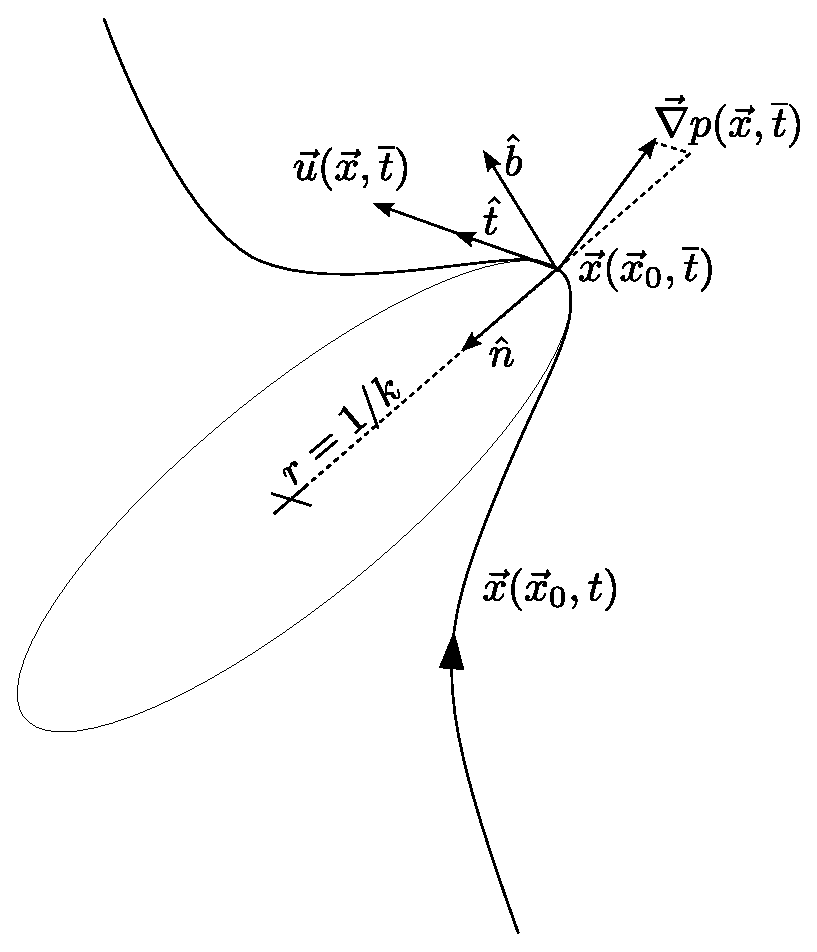
\includegraphics[width=1.0\textwidth]{./fig/frenet.eps}
\end{center}
\end{minipage}
\begin{itemize}
 \item la proiezione del termine forzante lungo la tangente alla traiettoria è la responsabile dell'accelerazione tangenziale della particella materiale;
 \item la proiezione del termine forzante lungo la normale alla traiettoria è la responsabile dell'accelerazione centripeta della particella maetriale e, di conseguenza, della curvatura della traiettoria;
 \item la proiezione della forzante lungo la direzione binormale è nulla.
\end{itemize}

\noindent
In assenza di forze di volume ($\bm{f}=0$) e sforzi viscosi
($\mathbb{T}=\mathbb{S}-p\mathbb{I}=-p\mathbb{I}$):
\begin{equation}
 \begin{cases}
  \rho \frac{dv}{dt} = - \bm{\hat{t}} \cdot \bm{\nabla} p \\
  \rho v^2 k         = - \bm{\hat{n}} \cdot \bm{\nabla} p \\
  0                  = - \bm{\hat{b}} \cdot \bm{\nabla} p \\
 \end{cases}
\end{equation}
%
e quindi:
\begin{itemize}
 \item l'accelerazione tangenziale è proporzionale alla proiezione del gradiente di pressione in direzione tangente alla tratiettoria;
 \item l'accelerazione centripeta, $v^2/r = v^2 k$, è proporzionale alla proiezione del gradiente di pressione in direzione normale alla tratiettoria. Il termine $\rho v^2 k$ è sempre positivo poichè prodotto di quantità positive: la curvatura di una linea è non negativa per come è definita, la densità è positiva, il modulo di un vettore è anch'esso non negativo. Il prodotto scalare tra la normale e il gradiente della pressione (derivata direzionale della pressione in direzione $\bm{\hat{n}}$) deve quindi essere negativo. La pressione quindi diminuisce, andando verso il centro del cerchio osculatore. Sempre dalla seconda equazione è immediato notare che la curvatura della traiettoria è proporzionale alla componente del gradiente di pressione lungo il versore normale;
 \item la proiezione del gradiente di pressione in direzione binormale a una traiettoria è nullo.
\end{itemize}
% Un'analisi della componente normale permette di ricavare, \textbf{sotto le
%  ipotesi fatte}, il legame tra la curvatura delle traiettorie delle
%  particelle fluide e il gradiente del campo di pressione.
% Il termine a sinistra dell'uguale è positivo
% La componente tangente fa aumentare 
%  il modulo della velocità, mentre la componente binormale deve essere nulla.
%Essendo il versore $\bm{\hat{n}}$ diretto verso il centro del cerchio
% osculatore (in parole povere è diretta verso l'interno della curva),
% la curvatura $k$ positiva, segue che la pressione deve diminuire lungo 
% $\bm{\hat{n}}$, cioè aumenta all'allontanarsi dal cerchio del centro
% osculatore (in parole altrettanto povere, ``verso l'esterno'').
%\textit{(Nemmeno a dirlo, la densità $\rho$ è positiva e il quadrato
%  del modulo della velocità $v^2$ è positivo.)}
%\noindent
%Dalla componente lungo $\bm{\hat{n}}$ si nota che il legame tra 
% la componente del gradiente della pressione in quella direzione è
% \textbf{proporzionale} alla curvatura della traiettoria della particella
% fluida.



\subsection{Vorticità}

L'equazione della vorticità in coordinate euleriane è
\begin{equation}
 \frac{\partial \bm{\omega}}{\partial t}
   + (\bm{u}\cdot\bm{\nabla}) \bm{\omega} =
 (\bm{\omega}\cdot\bm{\nabla}) \bm{u} + \nu \bm{\Delta} \bm{\omega}
\end{equation}

Se viene fatta l'ipotesi di viscosità nulla, il termine contenente il 
 laplaciano della vorticità non compare nell'equazione: questo termine
 è il responsabile della diffusione (isotropa per come è scritto) della
 vorticità.
 
L'equazione può essere quindi riscritta come:
 \begin{equation}
  \frac{D\bm{\omega}}{Dt} = (\bm{\omega} \cdot \bm{\nabla}) \bm{u}
 \end{equation}

\noindent 
Scritta in componenti
\begin{equation}
\begin{aligned}
  \frac{D \omega_i}{D t} = \omega_k \frac{\partial u_i}{\partial x_k} \\
\end{aligned}
\end{equation}

\noindent
Il termine di destra può essere riscritto come
\begin{equation}
\begin{aligned}
 \omega_k \frac{\partial u_i}{\partial x_k} & = 
 \omega_k \frac{\partial u_i}{\partial x_{0 l}}
      \frac{\partial x_{0 l}}{\partial x_k} = \qquad \qquad
      \left(u_i = \frac{D x_i}{D t}\right)  \\
 & = \omega_k \frac{D}{Dt} \left( \frac{\partial x_i}{\partial x_{0 l}}
    \right)\frac{\partial x_{0 l}}{\partial x_k} 
\end{aligned}
\end{equation}
Vale la relazione
\begin{equation}
 \frac{\partial x_i}{\partial x_{0 l}}
   \frac{\partial x_{0 l}}{\partial x_k} = \delta_{ik}
\end{equation}
Il termine di sinistra può essere riscritto come
\begin{equation}
 \frac{D \omega_i}{Dt} = \frac{D}{Dt} \left(\delta_{ik} \omega_k \right) =
 \frac{D}{Dt} \left( \frac{\partial x_i}{\partial x_{0 l}}
   \frac{\partial x_{0 l}}{\partial x_k} \omega_k \right)
\end{equation}

Inserendo nell'equazione della vorticità e sfruttando le proprietà
 della derivata del prodotto:
\begin{equation}
\begin{aligned}
 &  \frac{D}{Dt} \left(  \frac{\partial x_i}{\partial x_{0 l}}
   \frac{\partial x_{0 l}}{\partial x_k} \omega_k  \right)  - 
  \omega_k \frac{D}{Dt} \left( \frac{\partial x_i}{\partial x_{0 l}}
    \right)\frac{\partial x_{0 l}}{\partial x_k} = 0 \\
 &  \frac{\partial x_i}{\partial x_{0 l}} 
  \frac{D}{Dt} \left( \frac{\partial x_{0 l}}{\partial x_k} \omega_k
    \right) = 0
\end{aligned}
\end{equation}
Se la trasformazione non è singolare, risulta quindi
\begin{equation}
  \frac{D}{Dt} \left( \frac{\partial x_{0 l}}{\partial x_k} \omega_k
    \right) = 0  \quad \Rightarrow \quad
  \frac{\partial x_{0 l}}{\partial x_k} \omega_k = \omega_{l 0}
\end{equation}
e in conclusione, invertendo il gradiente della trasformazione delle
 coordinate
\begin{equation}\label{eqn:bilanci:vorticitàLagrange}
   \omega_k = \frac{\partial x_k}{\partial x_{0 l}}\omega_{l 0}
   \qquad , \qquad \bm{\omega} = \frac{\partial \bm{x}}{\partial \bm{x}_0}
      \bm{\omega}_0
\end{equation}

Si può quindi notare che la vorticità segue la stessa evoluzione
 di un segmento infinitesimo materiale, per il quale vale:
\begin{equation}
  d\bm{x} = \frac{\partial \bm{x}}{\partial \bm{x}_0}
      d\bm{x}_0
\end{equation}










 

\newpage
% Relazioni di salto
% \section{Relazioni di salto}

Si ricavano le condizioni di salto di velocità e sforzo in corrispondenza di superfici di interfaccia.
 Si sottolinea che queste superfici possono essere superfici introdotte dalla modellazione del problema,
 come ad esempio la superficie di separazione tra due fluidi all'interno della quale in generale agisce
 una tensione superficiale o una superficie di discontinuità tangenziale nel caso di fluido non viscoso,
 oppure superfici fittizie.
 
Si parte dai bilanci in forma integrale scritti per un volume in moto arbitrario. I bilanci di massa e quantità di moto
 del volume in moto arbitrario si ottengono dalle regole di derivazione su domini mobili delle funzioni
 $f = \rho$ e $\bm{f} = \rho \bm{u}$,
\begin{equation}
 \frac{d}{dt} \int_{V(t)} f dV 
    = \frac{d}{dt} \int_{v(t)=V(t)} f dv + \oint_{\partial v(t)=\partial V(t)} f(\bm{v}-\bm{w}) \cdot \bm{\hat{n}} ds 
\end{equation}
dove $\bm{u}$ è la velocità del fluido, $\bm{w}$ è la velocità della superficie di discontinuità.

Il billancio integrale viene fatto su un elemento di volume infinitesimo, ``allungato'' nelle direzioni della superficie.
 Quando il volume dell'elemento infinitesimo tende a zero, tende a zero più velocemente dei contributi sulle superfici
 parallele alla superficie di salto.
 
\begin{figure}[h]
\centering
%\captionsetup[subfigure]{labelformat=empty}
\subfloat[][Definizione delle velocità ai due lati dell'elemento infinitesimo e delle dimensioni dello stesso. La velocità 
    della superficie è indicata con $\bm{w}$.]
   {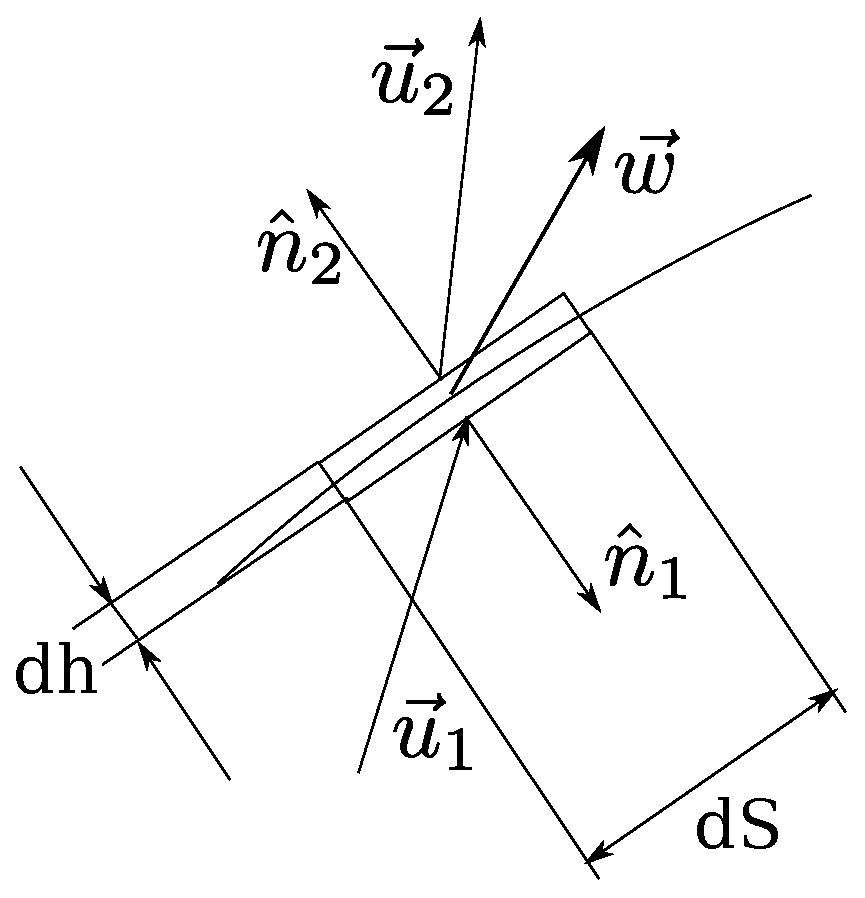
\includegraphics[width=0.30\textwidth]{./fig/elem_velocity.eps}} \qquad \qquad
\subfloat[][Definizione degli sforzi e della tensione superficiale agenti sull'elemento infinitesimo della superficie. ]
   {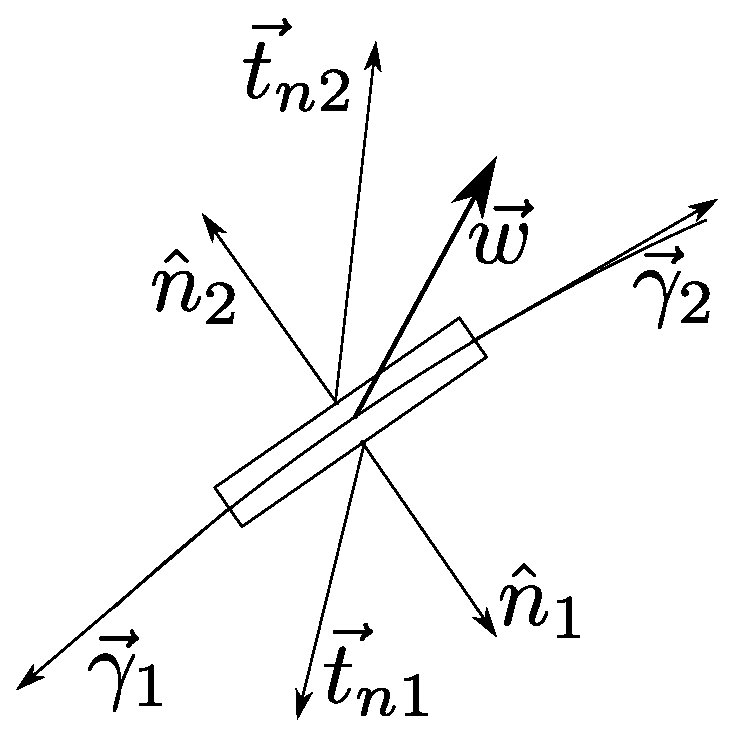
\includegraphics[width=0.30\textwidth]{./fig/elem_stress.eps}}
\end{figure}

L'elemento di volume $dv$ è il parallelepipedo di superfici laterali $dS$, paralleli alla superficie, e basi $dh$ perpendicolari
 alla superficie. Se si ipotizza che le superfici $dh \ll dS$ i contributi nei bilanci dei termini agenti sulle superfici $dh$
 (tranne che nel caso della tensione superficiale, che ha le dimensioni di uno sforzo per una lunghezza) sono trascurabili.


\subsection{Bilancio di massa}
Il bilancio di massa per il volume $dv$  in moto con velocità $\bm{w}$ è
\begin{equation}
 \dfrac{d}{dt}\int_{v} \rho + \oint_{\partial v} \rho (\bm{u} - \bm{w} ) \cdot \bm{\hat{n}} = 0
\end{equation}
Trascurando i contributi di volume e quelli delle superfici $dh$
\begin{equation}
 \rho_1 (\bm{u}_1 - \bm{w} ) \cdot \bm{\hat{n}}_1 dS +  \rho_2 (\bm{u}_2 - \bm{w} ) \cdot \bm{\hat{n}}_2 dS = 0
\end{equation}
dove le normali $\bm{\hat{n}}_1 = \bm{\hat{n}}$ e $\bm{\hat{n}}_2 = -\bm{\hat{n}}$ sono opposte. La quantità tra parentesi è la velocità relativa
 del fluido rispetto alla superficie. Si definisce quindi il flusso di massa $m$ attraverso la superficie.
\begin{equation}
\begin{aligned}
 - m & = \rho_1 (\bm{u}_1 - \bm{w} ) \cdot \bm{\hat{n}} = \rho_2 (\bm{u}_2 - \bm{w} ) \cdot \bm{\hat{n}} \\
   & = \rho_1  \bm{u}_{r1} \cdot \bm{\hat{n}} = \rho_2 \bm{u}_{r2} \cdot \bm{\hat{n}} \\
\end{aligned}
\end{equation}

\noindent
Nel caso di densità uniforme $\rho_1 = \rho_2 = \rho$ si ``conservano'' le componenti normali della velocità relativa e della
 velocità.
\begin{equation}
\begin{aligned}
  \bm{u}_{r1} \cdot \bm{\hat{n}} & = \bm{u}_{r2} \cdot \bm{\hat{n}} \\
  \bm{u}_{1}  \cdot \bm{\hat{n}} & = \bm{u}_{2}  \cdot \bm{\hat{n}} \\
\end{aligned}
\end{equation}


\subsection{Bilancio di quantità di moto}
Il bilancio della quantità di moto per l'elemento $dv$ è
\begin{equation}
 \dfrac{d}{dt}\int_{v} \rho\bm{u} + \oint_{\partial v} \rho \bm{u}(\bm{u} - \bm{w} ) \cdot \bm{\hat{n}} = \oint_{\partial v} \bm{t_n} + \int_{v} \rho \bm{g} + \int_{l} \bm{\gamma}
\end{equation}
avendo incluso anche eventuali termini di tensione superficiale, svolto 
 sulla curva che separa tre sostanze (come ad esempio il ``perimetro''
 del menisco visto nell'esercizio sul capillare: in quel caso la curva
 $l$ separa il liquido, dall'aria, dalle pareti solide del capillare).
Trascurando i termini di volume, il bilancio per l'elemento infinitesimo (per semplicità pensato in 2 dimensioni) è
\begin{equation}
 \rho_1 \bm{u}_1 (\bm{u}_1 - \bm{w})\cdot \bm{\hat{n}}_1 ds + \rho_2 \bm{u}_2 (\bm{u}_2 -\bm{w}) \cdot \bm{\hat{n}}_2 ds =
    \bm{t_{n1}} ds + \bm{\gamma}_1  + \bm{t_{n2}} ds + \bm{\gamma}_2 
\end{equation}
con $\bm{\gamma}_1 = \gamma \bm{\hat{t}_1}$, $\bm{\gamma}_2 = (\gamma + \gamma_{/s} ds) \bm{\hat{t}_2}$. I versori 
 tangenti $\bm{\hat{t}}_1$, $\bm{\hat{t}}_2$ agli estremi dell'elementino di superficie non sono allineati a causa della curvatura della superficie (si
rimanda alla ``dimostrazione'' della legge di Young-Laplace). Si tiene conto di una possibile
 variazione della tensione superficiale. Questa di solito può essere
 dovuta a differenze di temperatura o composizioni chimiche (perchè si
usa il sapone per lavarsi le mani?): si rimanda al 
 simpatico (?) video delle barchette sul fondo del documento della dimostrazione
 della legge di Young-Laplace, nel quale viene usata una ``propulsione a effetto Marangoni'' per barchette di carta. Il contributo della tensione superficiale si può scrivere come
\begin{equation}
 \bm{\gamma}_2 + \bm{\gamma}_1 = (2 \gamma H \bm{\hat{n}} + \bm{\nabla}_2 \gamma )ds
\end{equation}
dove
\begin{itemize}
 \item H è la curvatura media $H = \frac{1}{2}\left(\frac{1}{R_1} + \frac{1}{R_2}\right)$ nel caso tridimensionale, che nel caso bidimensionale
 coincide con $ \frac{1}{2 R}$ (uno dei due raggi di curvatura diventa infinito).
 \item $\bm{\hat{n}}$ è il vettore normale che punta verso i centri di
 curvatura.
 \item $\bm{\nabla}_2$ è il gradiente ristretto alla superficie, tangente ad essa.
\end{itemize}

\noindent
Ricordando la definizione di $m$ e inserendola nel bilancio
\begin{equation}
 m ( \bm{u}_1 - \bm{u}_2 ) =
    \bm{t_{n1}} + \bm{t_{n2}} + 2 \gamma H \bm{\hat{n}} + \bm{\nabla}_2 \gamma
\end{equation}

\noindent
Si analizzano ora alcuni casi particolari:
\begin{itemize}
\item Statica con tensione superficiale. La velocità è nulla ovunque, i vettori di sforzo hanno solo il contributo della pressione
 $\bm{t_n} = -p \bm{\hat{n}}$. Secondo queste ipotesi, non si possono avere contributi tangenziali nemmeno a causa della tensione 
 superficiale e quindi $\gamma$ deve essere uniforme sulla superficie. Nel caso bidimensionale si ricorda che la normale $\bm{\hat{n}}$
 punta verso il centro del cerchio osculatore e coincide quindi con la normale $\bm{\hat{n}}_1$ dell'immagine e il raggio di curvatura $R$ è positivo.
 Il bilancio della quantità di moto si riduce all'equilibrio statico della superficie
 \begin{equation}
   p_1 - p_2 = \frac{\gamma}{R}
 \end{equation}
 Si osserva quindi che la pressione ``interna'' $p_1$ deve essere maggiore di $p_2$.
\item Fluido inviscido, superficie senza tensione superficiale. Il bilancio si riduce a 
\begin{equation}
  m ( \bm{u}_1 - \bm{u}_2 ) = - (p_1 - p_2) \bm{\hat{n}}
\end{equation}
\item Fluido inviscido, superficie senza tensione superficiale, densità uniforme. Si è visto come la 
  velocità (e le velocità relative) normali alla superficie devono essere uguali da entrambe le parti
  della superficie. %Se la superficie è una superficie materiale, la velocità della superficie coincide
%  con quella del fluido e quindi la velocità relativa è nulla ed $m = 0$.
%  Risulta quindi che non ci può essere salto di pressione attraverso una tale superficie (questo è quello che significa
%  l'ipotesi espressa in termini pittoreschi di ``scia scarica'' nell'aerodinamica a potenziale).
%  \begin{equation}
%    p_1 = p_2
%  \end{equation}
  Se si ipotizza che la superifice non sia attraversata da flusso di massa (si impone che la componente normale della velocità relativa sia nulla,
  non la velocità relativa nel suo complesso). In questo caso non è possibile trovare una relazione 
  di salto per la velocità tangenziale (o almeno questo non è possibile se non si aggiungono altre ipotesi o altre equazioni \dots vedremo 
  un caso semplificato applicando il teorema di Bernoulli a un problema aerodinamico bidimensionale stazionario \dots):
  poichè $m=0$ la superficie è ``scarica'' (capiterà nei prossimi corsi di sentir parlare o aver direttamente a che fare con ``
  l'ipotesi di scia scarica'': questa non dovrà quindi essere una novità o una sorpresa in futuro)
  \begin{equation}
    p_1 = p_2
  \end{equation}
  ma non si riesce a ricavare nessuna informazione dalla componente tangenziale
  dell'equazione poichè è un'identità $0=0$ a prescindere dal valore di $( \bm{u}_1 - \bm{u}_2 )\cdot \bm{\hat{t}}$. Attraverso tale superficie
  (di spessore nullo) ci può essere un salto finito di velocità tangenziale: in questo caso la superficie è una superficie di vorticità infinita
\end{itemize}

\noindent
L'ultimo caso particolare verrà utilizzato in qualche esercizio in cui un dominio occupato da un fluido può essere suddiviso in un sottodominio 
 nel quale è valido il teorema di Bernoulli (in qualche forma \dots) e in un sottodominio dove sono valide le relazioni della statica: le condizioni
 di salto serviranno a far comunicare tra di loro i due sottodomini (e a risolvere correttamente l'esercizio).

\subsection{Bilancio di energia}
Non verrà detto nulla sulle relazioni di salto delle altre quantità \dots

 
\newpage

% Esercizi
%> === Bilancio di massa ========================================
\noindent
\begin{tabular}{cc}
\begin{minipage}{0.65\textwidth}
\begin{exerciseS}[Bilancio di massa: teoria delle reti]
Si consideri  una rete idraulica come quella rappresentata in figura.
All'interno dei tubi scorre acqua. Sia nota le velocit\`a media
dell'acqua all'interno di alcuni dei rami della rete: 
$U_1 = 1\, m/s$, $U_2 = 1.5\, m/s$, $U_3 = 0.5\, m/s$,
$U_7 = 2\, m/s$ e $U_8 = 0.3\, m/s$. 
Il verso della velocit\`a è indicato dalle frecce 
sul disegno.
Determinare la portata volumetrica, la portata in massa e la velocit\`a
media all'interno di ciascun ramo della rete 
sapendo che l'acqua ha una densit\`a pari a $\overline{\rho} = 999\ kg/m^3$,
e che il diametro dei tubi \`e rispettivamente $D_1=0.4\ m$, 
$D_2=0.2\ m$, $D_3=0.2\ m$, $D_4=0.3\ m$, $D_5=0.5\ m$,
$D_6=0.25\ m$, $D_7=0.3\ m$, $D_8=0.6\ m$.

($Q_1 = 0.13\ m^3/s$, $Q_2 = 0.05\ m^3/s$, $Q_3 = 0.02\  m^3/s$, 
 $Q_4 = 0.13\ m^3/s$, $Q_5 = 0.06\ m^3/s$, $Q_6 = 0.13\  m^3/s$, 
 $Q_7 = 0.14\ m^3/s$, $Q_8 = 0.08\ m^3/s$,
 $U_1 = 1\ m^3/s$, $U_2 = 1.5\  m^3/s$, $U_3 = 0.5\  m^3/s$, 
 $U_4 = 1.87\ m^3/s$, $U_5 = 0.29\  m^3/s$, $U_6 = 2.69\  m^3/s$, 
 $U_7 = 2\  m^3/s$, $U_8 = 0.3\ m^3/s$,
 $\overline{Q}_1 = 125.5\  kg/s$, $\overline{Q}_2 = 47.08\  kg/s$,
 $\overline{Q}_3 = 15.69\  kg/s$, 
 $\overline{Q}_4 = 131.8\  kg/s$, $\overline{Q}_5 = 54.49\  kg/s$,
 $\overline{Q}_6 = 131.8\  kg/s$, 
 $\overline{Q}_7 = 141.2\  kg/s$, $\overline{Q}_8 = 84.74\  kg/s$)
\end{exerciseS}
\end{minipage}
&
\begin{minipage}{0.35\textwidth}
   \begin{center}
   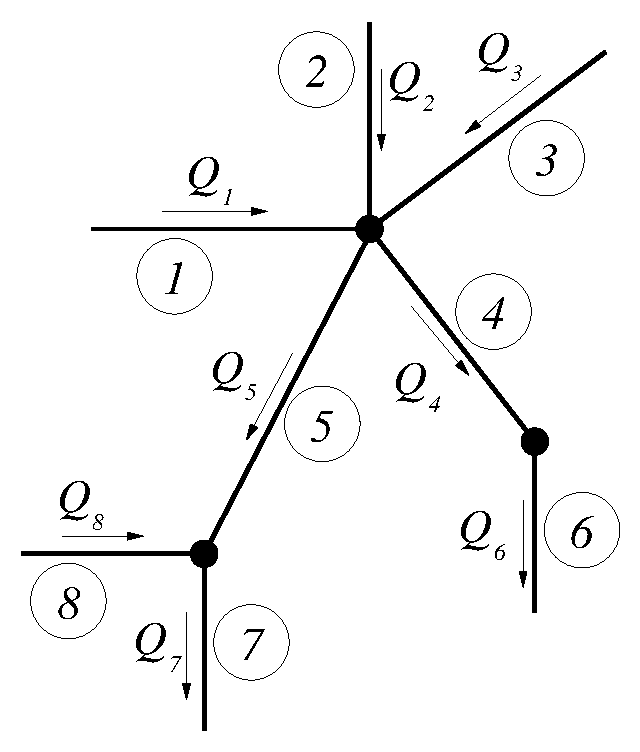
\includegraphics[width=0.90\textwidth]{./fig/rete.eps}
   \end{center}
\end{minipage}
\end{tabular}

\sol

\partone
Bilancio integrale della massa. Teoria delle reti: bilancio ai nodi.

\parttwo
Se il regime di moto è stazionario, la portata massica è costante e indipendente dalla sezione considerata all'interno di ogni singolo tubo. Il bilancio di massa nell'$i$-esimo tubo è,
\begin{equation}
 \underbrace{\dfrac{d}{dt} \int_{V_i} \bm{\rho}}_{=0} = \oint_{S_i} \rho \bm{u} \cdot \bm{\hat{n}} = \oint_{S_{i,{\alpha}}}\rho \bm{u} \cdot \bm{\hat{n}} + \oint_{S_{i,\beta}} \rho \bm{u} \cdot \bm{\hat{n}} = \tilde{Q}_{i,\alpha} + \tilde{Q}_{i,\beta} \quad \rightarrow \quad \tilde{Q}_{i,\alpha} = -  \tilde{Q}_{i,\beta} \ , 
\end{equation}
avendo indicato $S_{i,{\alpha}}$ e $S_{i,{\beta}}$ le due sezioni in ``ingresso'' e ``uscita'' del tubo $V_i$, con $\bm{\hat{n}}$, $\tilde{Q}_{\alpha}$ e $\tilde{Q}_{\beta}$ la normale uscente e i flussi di massa uscenti dal volume $V_i$. Se si calcola il flusso di massa $\overline{Q}_i$ attraverso le sezioni del tubo con normale identificata dal ``verso di percorrenza'' del tubo, uno dei due termini cambia segno e si dimostra che la portata è costante sulle sezioni del singolo tubo, 
\begin{equation}
 \overline{Q}_{i,\alpha} = \overline{Q}_{i,\beta} =: \overline{Q}_{i} \ .
\end{equation}
%
Utilizzando il verso delle frecce indicato in figura per stabilire il segno dei flussi di massa, il bilancio di massa ai nodi porta al sistema lineare,
\begin{equation}
 \begin{cases}
   \overline{Q}_1 + \overline{Q}_2 + \overline{Q}_3 - \overline{Q}_4 - \overline{Q}_5 = 0 & \text{(bil. al nodo in alto)} \\
   \overline{Q}_5 + \overline{Q}_8 - \overline{Q}_7 = 0 & \text{(bil. al nodo a sinistra)} \\
   \overline{Q}_4 - \overline{Q}_6 = 0 & \text{(bil. al nodo a destra)} \ , \\
 \end{cases}
\end{equation}
nel quale le incognite sono i flussi $\overline{Q}_4$, $\overline{Q}_5$, $\overline{Q}_6$, una volta calcolati gli altri flussi con i dati forniti dal testo del problema,
$\overline{Q}_k = \rho \frac{\pi}{4}D_k^2 U_k$, $k=1,2,3,7,8$.
%
Successivamente si calcolano le portate volumetriche $Q_k$ incognite, dividendo le portate massiche $\overline{Q}_k$ per la densità $rho$,
\begin{equation}
 Q_k = \dfrac{\overline{Q}_k}{\rho} \quad , \quad k = 1:8 \ .
\end{equation}

%\begin{equation}
% \begin{cases}
%   Q_1 + Q_2 + Q_3 - Q_4 - Q_5 = 0 & \text{(bil. al nodo in alto)} \\
%   Q_5 + Q_8 - Q_7 = 0 & \text{(bil. al nodo a sinistra)} \\
%   Q_4 - Q_6 = 0 & \text{(bil. al nodo a destra)} \\
% \end{cases}
%\end{equation}

%\item
%Si ricavano le velocità ancora incognite:
%\begin{equation}
%  U_i = \frac{Q_i}{S_i}, \qquad i = 4,5,6
%\end{equation}

%\item
%Infine si calcolano le portate in massa semplicemente moltiplicando 
%quelle volumetriche per la densità $\bar{\rho}$:
%\begin{equation}
%  \bar{Q_i} = \bar{\rho} Q_i, \qquad i = 1:8
%\end{equation}

%\end{itemize}
 % teoria delle reti
\newpage
\noindent
\begin{tabular}{cc}
\begin{minipage}{0.95\textwidth}
\begin{exerciseS}[Bilancio di massa: riempimento bombola]
Si sta riempiendo una bombola per immersioni subacquee.
Sapendo che la pompa aspira aria a pressione ambiente di 
$1.01\times10^5\ Pa$ e alla temperatura di $293\ K$
in un condotto di sezione $1\ cm^2$ in cui la velocit\`a media \`e di 
$0.5\ m/s$ e che non ci sono perdite nel sistema di pompaggio,
determinare la rapidit\`a di variazione della massa d'aria e della sua 
densit\`a all'interno della bombola, sapendo che il volume della bombola
\`e pari a $0.02 \  m^3$.

($\frac{dM}{dt} = 6.01 \times 10^{-5}\ kg/s, \frac{d \rho}{d t} = 3.00 \times 10^{-3}\ kg/(m^3 s)$).
\end{exerciseS}
\end{minipage}
\end{tabular}

\sol

\partone Bilancio integrale della massa. Legge dei gas perfetti.

\parttwo
Sono date la pressione $p$ e la temperatura $T$ all'uscita della pompa.
\'E nota l'area $S$ della sezione e la velocità media $U$ su quella
 sezione. 
% Se si suppone che il gas sia un gas ideale perfetto, si può ricavare la densità come $\rho = \frac{p}{R T}$. Si può quindi calcolare il flusso di massa $\dot{m}$.
%
Si trova la variazione di massa all'interno della bombola grazie al bilancio integrale di massa nel volume della bombola $V$ (volume di controllo, fisso),
\begin{equation}
 \dfrac{d M}{d t} = \dfrac{d}{d t} \int_V \rho = -\oint_S \rho \bm{u} \cdot \bm{u} =
 \rho_{in} S_{in} U \ ,
\end{equation}
dove si è indicato con $M$ la massa totale, $S_{in}$ l'area della sezione del tubo utilizzato per riempire la bombola e $\rho_{in}$, la densità sulla sezione di ingresso, dove sono note la pressione $P_{in}$ e la temperatura $T_{in}$. Ipotizzando che valga la legge di stato dei gas perfetti, la densità sulla sezione di ingresso vale
\begin{equation}
 \rho_{in} = \dfrac{P_{in}}{R T_{in}} \ ,
\end{equation}
dove $R=287 J/(kg\ K)$ è la costante dei gas per l'aria. La derivata nel tempo della massa d'aria nella bombola vale quindi
\begin{equation}
  \frac{d M}{d t} = 6.0 \cdot 10^{-5} \dfrac{kg}{s} \ .
\end{equation}
%
Supponendo che la densità dell'aria si uniforme all'interno della bombola, si può calcolare la sua derivata nel tempo, 
\begin{equation}
 \dfrac{d \rho}{d t} = \dfrac{1}{V} \dfrac{d}{dt} \int_V \rho = 2.0 \cdot 10^{-3} \dfrac{kg}{m^3 s} \ .
\end{equation}


%\begin{equation}
%  \dot{m} = \rho S U
%\end{equation}

%La derivata della massa contenuta nella bombola è uguale al flusso entrante nella bombola, uguale al flusso uscente dalla pompa (nell'ipotesi che non ci siano perdite).

%\begin{equation}
% \frac{d M}{d t} = \rho S U  \quad \Rightarrow \quad
%  \frac{d M}{d t} = 6.0 \cdot 10^{-5} kg/ s
%\end{equation}

%Per calcolare la derivata della densità all'interno della bombola, si 
%osserva che il volume della bombola non cambia. La derivata della 
%massa è $\frac{d M}{d t} = \frac{d (\rho V)}{d t} = V \frac{d \rho}
%{d t}$.

%\begin{equation}
% \frac{d \rho}{d t} = \frac{\rho U S}{V} \quad \Rightarrow \quad
%  \frac{d \rho}{d t} = 2.0 \cdot 10^{-3} kg/(m^3 s)
%\end{equation}
 % riempimento bombola

%> === Bilancio di quantità di moto e risultante sui corpi ======
\newpage

\noindent
\begin{tabular}{cc}
\begin{minipage}{0.60\textwidth}
\begin{exerciseS}[Effetto Coanda sul cilindro]
Un getto d'acqua ($\rho=999\ kg/m^3$) stazionario, piano e orizzontale 
viene indirizzato su un cilindro, lambendone la superficie e
venendo deviato di un angolo $\alpha =15^\circ$.
Determinare la forza agente su una porzione del cilindro di lunghezza 
pari a $H = 2\ m$, dovuta sia al getto d'acqua,
sia all'aria circostante, sapendo che:
\begin{itemize}
  \item il fluido che circonda il getto e il cilindro \`e aria in quiete a
  pressione atmosferica di $101325\ Pa$;
  \item la larghezza del getto \`e $h=2\ cm$;
  \item la portata d'acqua per unit\`a di lunghezza nel getto \`e 
  $Q = 199\ kg\ m^{-1}\ s^{-1}$.
\end{itemize}
Sufficientemente lontano dal cilindro, il profilo di velocità sulle sezioni del getto è uniforme. Illustrare tutte le ipotesi semplificative adottate nella risoluzione dell'esercizio.

($\bm{F} = 1026\ \hat{\bm{x}} - 135\ \hat{\bm{y}} \ N$)
\end{exerciseS}
\end{minipage}
&
\begin{minipage}{0.35\textwidth}
   \begin{center}
   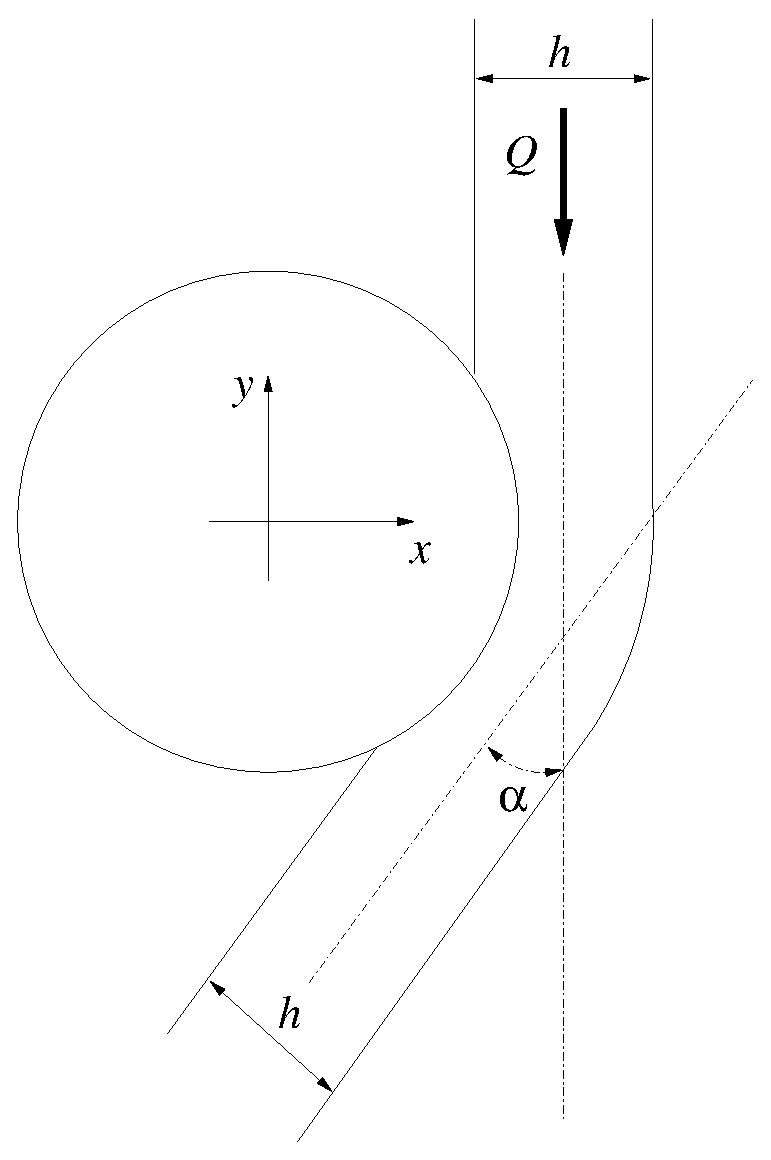
\includegraphics[width=0.90\textwidth]{./fig/coanda.eps}
   \end{center}
\end{minipage}
\end{tabular}

\vspace{1.0cm}

\sol

\partone
  Bilanci integrali di massa e quantità di moto. Equazioni di equilibrio (equazioni fondamentali della dinamica classica). Principio di azione e reazione. Integrale della normale su una superficie chiusa è identicamente nullo. Effetto Coanda (esempio della bustina da té sotto il rubinetto).

\parttwo
Vengono fatte alcune ipotesi: il problema stazionario; attorno al getto e al solido, l'aria è in quiete con pressione uniforme $p_a$; il profilo di velocità è uniforme sulle sezioni del getto considerate nelle equazioni di bilancio.

Partendo dalle equazioni di bilancio per il volume di controllo $V_{f}$ occupato dal fluido,  rielaborando il termine degli sforzi di superficie sforzi di superficie, si ricava la risultante $\bm{R}$ agente sul solido in funzione del flusso di quantità di moto del fluido attraverso la superficie $S_{f} = \partial V_f$.

Innanzitutto viene ricavata l'espressione della risultante $\bm{R}$ agente sul solido. 
\begin{itemize}
 \item Vengono scritte le equazioni di bilancio per il fluido, considerando il volume $V_f$
   \begin{equation}
     \begin{cases}
       \dfrac{d}{d t} \displaystyle\int_{V_f} \rho + \oint_{S_f} \rho \bm{u} \cdot \hat{\bm{n}} = 0 & \qquad \text{(massa)} \\
       \dfrac{d}{d t} \displaystyle\int_{V_f} \rho \bm{u} + \oint_{S_f} \rho \bm{u} \bm{u} \cdot \hat{\bm{n}} =
        \oint_{S_f} \bm{t_n} = 0  
%        \oint_{\partial \Omega} p \hat{\bm{n}} - \oint_{\partial \Omega} \bm{s_n} = 0  
        & \qquad \text{(quantità di moto)}  %\Rb^{ext}
      \end{cases}
    \end{equation}
 \item Viene introdotta l'ipotesi di stazionarietà del fenomeno, $\frac{d}{dt}\equiv 0$.
 La risultante degli sforzi viene scritta come somma degli sforzi di pressione e degli sforzi viscosi, 
\begin{equation}
\begin{split}
% & \Rb = \oint_{S_{cyl}}  {\bm{t}}_{\bm{n}} = 
% \oint_{S_{cyl}}  {\bm{s}}_{\bm{n}} - \oint_{S_{cyl}} p {\hat{\bm{n}}}_{cyl} \\
 & \oint_{S_f} \rho \bm{u} \bm{u} \cdot \hat{\bm{n}} 
  = \oint_{S_{f}}  {\bm{t}}_{\bm{n}} = 
 \oint_{S_{f}}  {\bm{s}}_{\bm{n}} - \oint_{S_f} p {\hat{\bm{n}}}_{f} \ .
\end{split}
\end{equation}

%\begin{equation}
%  \Rb = \oint_{S_{cyl}} \bm{t_n} = 
%  \int_{S_{ext}} \bm{t_n} + \int_{S_{c}} \bm{t_n} = 
%  - \int_{S_{ext}} p \bm{n}_{cyl} + \int_{S_{c}} \bm{t_n} = 
%\end{equation}


\item Viene manipolato il termine degli sforzi di superficie. Il contorno $S_f$ del volume fluido viene scomposto come unione della superficie a contatto con il solido $S_{fs}$, delle superfici ``laterali'' $S_{f\ell}$ (attraverso le quali non c'è flusso di quantità meccaniche, poichè $\bm{u}\cdot\bm{\hat{n}} = 0$) a contatto con l'aria in quiete e le sezioni ``di ingresso'' $S_{f,1}$ e ``di uscita'' $S_{f,2}$ sulle quali la velocità è uniforme, utilizzate per i bilanci integrali per il volume fluido. Viene indicata con $\bm{\hat{n}_f}$ la normale uscente dal volume $V_f$.
Il contorno $S_s$ del solido viene scomposto come unione della superficie a contatto con il fluido $S_{sf}$ e della superficie $S_{s\ell}$ a contatto con l'aria in quiete. Viene indicata con $\bm{\hat{n}_s}$ la normale uscente dal volume $V_s$.
In questo modo, la superficie $S_{fs}$ coincide con la superficie $S_{sf}$, a meno della normale invertita, $\bm{\hat{n}_f} = \bm{\hat{n}_s}$. Su queste superfici, per il terzo principio della dinamica, lo sforzo ${\bm{t_n}}_{sf}$ agente sul solido dovuto al fluido è uguale e contrario allo sforzo ${\bm{t_n}}_{fs}$ agente sul fluido dovuto al fluido, ${\bm{t_n}}_{sf}=-{\bm{t_n}}_{fs}$.
 La superficie formata dall'unione $S_{f\ell} \cup S_{f,1} \cup S_{f,2} \cup S_{s\ell} =:S_{ext}$ è una superficie chiusa con normale uscente $\bm{\hat{n}}$ uguale a $\bm{\hat{n}_f}$ sulle prime tre superfici e uguale a $\bm{\hat{n}}$ su $S_{s\ell}$. Lo sforzo agente su $S_{ext}$ è uguale a $-p_a\bm{\hat{n}}$, poiché le superfici libere sono a contatto con aria in quiete con pressione $p_a$ e le traiettorie delle particelle rettilinee (senza curvatura\footnote{Vedi commento sull'equazione della quantità di moto e sulle traiettorie delle particelle}) sulle sezioni $S_{f,1}$ e $S_{f,2}$.
%Si indica con $S_f$ il contorno fluido: questo è costituito dall'unione del controno a contatto con il cilindro $S_c$ e quella "libera" $S_l$. Il contorno del cilindro $S_{cyl}$ è suddiviso nel contorno $S_c$ a contatto con il fluido e nel contorno libero $S_{c_l}$.

%Nei passaggi successivi si ricava il legame tra sforzi sul contorno del dominio fluido e la forza agente sul cilindro.
%Si usa le ipotesi che sulle superfici libere agisca solo la pressione ambiente. Si usa il fatto che l'integrale di una quantità costante per la normale su una superficie chiusa è nullo. Si usa infine il fatto che $\bm{n}=-\bm{n}_{cyl}$ (normali uscenti dai due domini, uguali e contrarie) e
%$\bm{t_n}=-\bm{t}_{\bm{n}_{cyl}}$ (sforzi agenti sulla superficie comune, uguali e contrari).


\begin{equation}
\begin{aligned}
  \oint_{S_f} \bm{t_n} & = 
  \int_{S_{f\ell}} \bm{t_n} + \int_{S_{f,1+2}} \bm{t_n} + \int_{S_{fs}} \bm{t_n} = & \text{($\bm{t_n} |_{S_{f\ell},S_{f,1+2}} = -p_a \bm{\hat{n}_f}$ )}\\
  & = - \int_{S_{f\ell}\cup S_{f,1+2}} p_a \bm{\hat{n}_f} + \int_{S_{fs}} \bm{t_n} = & \text{(somma e sottrazione di $\int_{S_{fs}} p_a \bm{\hat{n}_f}$)}\\
  & = \underbrace{- \int_{S_{f\ell}\cup S_{f,1+2}} p_a \bm{\hat{n}_f} - \int_{S_{fs}} p_a \bm{\hat{n}_f}}_{-\oint_{S_f} p_a \bm{\hat{n}_f}=0}
  + \int_{S_{fs}} p_a \bm{\hat{n}_f} + \int_{S_{fs}} \bm{t_n} = & \text{($\bm{\hat{n}_f} = -\bm{\hat{n}_s}$, ${\bm{t_n}}_{fs} = - {\bm{t_n}}_{sf}$ su $S_{fs}$)} \\
  & = - \int_{S_{sf}} p_a \bm{\hat{n}}_{s} - \int_{S_{sf}} {\bm{t_n}}_{sf} = &
   \text{($\oint_{S_s=S_{sf}\cup S_{s\ell}} p_a \bm{\hat{n}_s} = 0)$} \\
  & = + \int_{S_{s\ell}} p_a \bm{\hat{n}}_{s} - \int_{S_{sf}} {\bm{t_n}}_{sf} = &
   \text{(${\bm{t_n}}_s = -p_a\bm{\hat{n}_s}$ su $S_{s\ell}$} \\
  & = - \int_{S_{s\ell}} {\bm{t_n}}_{s} - \int_{S_{sf}} {\bm{t_n}}_{sf} = - \oint_{S_{s}} {\bm{t_n}}_{s} = \\
%  \text{($S_{cyl} = S_c \cup S_{c_l}$ e $\int_{S_{cyl}} p_a \bm{n} = 0$)}\\
%  & = \int_{{S_c}_l} p_a \bm{n}_{cyl} + \int_{S_c} \bm{t_n} = &
%  \text{($\bm{t}_{\bm{n}_{s}}|_{S_{c_l}} = -p_a \bm{n}_{cyl}$, $\bm{t}_{\bm{n}_{cyl}}|_{S_c} = - \bm{t_n}$)} \\
%  & = - \int_{{S_c}_l} \bm{t}_{\bm{n}_{cyl}} - \int_{S_c} \bm{t}_{\bm{n}_{cyl}} = \\
%  & = - \int_{S_{cyl}} \bm{t}_{\bm{n}_{cyl}} \\
  & = - \bm{R} \ ,
\end{aligned}
\end{equation}
dove $\bm{R}$ è la risultante degli sforzi di superficie agente sul solido. In questo esercizio è il contributo delle forze di volume (ad esempio il peso) agenti sul solido.
% \item Riscrittura integrali di contorno % della pressione
%
%\begin{equation}
%\begin{split}
%  & \oint_{S_{cyl}} p {\hat{\bm{n}}}_{cyl} = 
%   \int_{S_c} (p-p_0) {\hat{\bm{n}}}_{cyl}
%   + \oint_{S_{cyl}} p_0 {\hat{\bm{n}}}_{cyl} =
%   \int_{S_c} (p-p_0) {\hat{\bm{n}}}_{cyl} \\
%  & \oint_{S_{f}} p {\hat{\bm{n}}} = 
%   \int_{S_c} (p-p_0) {\hat{\bm{n}}}
%   + \oint_{S_{f}} p_0 {\hat{\bm{n}}} =
%   \int_{S_c} (p-p_0) {\hat{\bm{n}}} = - \int_{S_c} (p-p_0) {\hat{\bm{n}}}_{cyl}\\   
%\end{split}
%\end{equation}


%\item Le relazioni semplificate vengono inserite nelle equazioni di equilibrio; si può scrivere quindi:
%\begin{equation}
%\begin{split}
%  \Rb & = - \oint_{S_{cyl}} p {\hat{\bm{n}}}_{cyl} = 
%   - \oint_{S_{c}} (p-p_0) {\hat{\bm{n}}}_{cyl} = 
%   \oint_{S_{c}} (p-p_0) {\hat{\bm{n}}} = 
%   -\oint_{S_f} \rho \bm{u} \bm{u} \cdot \hat{\bm{n}}
%\end{split}
%\end{equation}

\item Sostituendo nell'equazione del bilancio della quantità di moto si ottiene:
\begin{equation}
  \bm{R} = - \oint_{S_f} \rho \bm{u} \bm{u} \cdot \hat{\bm{n}} 
\end{equation}

\item Considerando solo le superfici di $V_f$ attraverso le quali c'è un flusso non nullo di quantità di moto, la risultante delle forze diventa
\begin{equation}
 \bm{R} = - \int_{S_{f,1}} \rho \bm{u} \bm{u} \cdot \hat{\bm{n}} 
          - \int_{S_{f,2}} \rho \bm{u} \bm{u} \cdot \hat{\bm{n}} 
\end{equation}
dove le quantità all'interno degli integrali sono riferite alle superfici di integrazione.
Sulle sezioni $S_{f,1}$, $S_{f,2}$ la velocità è uniforme con modulo $U$ (dalla continuità, la velocità sulle due sezioni è uguale poichè l'area delle due sezioni è uguale) diretta lungo la linea media del getto. Le componenti cartesiane della risultante $\bm{R}$ sono  
\begin{equation}
\begin{split}
  & R_x = \frac{Q^2 H}{\rho h} \sin \alpha \\
  & R_y = - \frac{Q^2 H}{\rho h} (1-\cos \alpha) \ ,
\end{split}
\end{equation} 
 riferite agli assi rappresentati in figura.
% L'area della sezione è $A = H h$ e la portata per unità di larghezza è $Q = \rho U h$ (quindi $\rho U^2 A = \frac{Q^2 H }{\rho h}$).

%Si scrive l'equazione precedente in componenti, proiettando lungo gli assi:



\end{itemize}
 % cilindro (Coanda)
\newpage

\noindent
\begin{tabular}{cc}
\begin{minipage}{0.60\textwidth}
\begin{exerciseS}[Giochi d'acqua]
Un getto d'acqua ($\rho=999\ kg/m^3 $) stazionario, piano e verticale 
viene indirizzato su un oggetto di massa $M$, tenuto da esso in equilibrio.
 Il getto ha distribuzione di velocità uniforme $U$ lungo lo spessore $H$, 
 mentre la distribuzione sul bordo dell'oggetto è 
triangolare di spessore $h$ con velocità massima $V$. Si calcoli la velocità $V$
e la massa $M$ dell'oggetto supponendo che:
\begin{itemize}
  \item il fluido che circonda il getto e il solido \`e aria in quiete a
  pressione atmosferica di $P_a = 101325\  Pa$;
  \item si possa trascurare la gravità nel bilancio di quantità di moto, ma non
nell'equilibrio del corpo.
\end{itemize} 


($V = U H / h ; M = \rho U^2 H / g$)
\end{exerciseS}
\end{minipage}
&
\begin{minipage}{0.35\textwidth}
   \begin{center}
   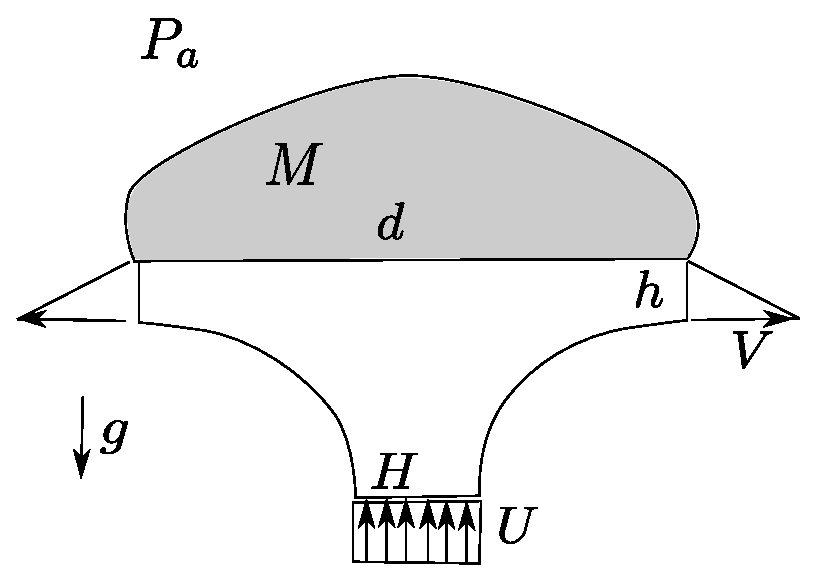
\includegraphics[width=0.90\textwidth]{./fig/gettoPiattello.eps}
   \end{center}
\end{minipage}
\end{tabular}

\vspace{1.0cm}

\sol

\partone
  Bilanci integrali di massa e quantità di moto. Equazioni di equilibrio (equazioni fondamentali della dinamica classica). Principio di azione e reazione. Integrale della normale su una superficie chiusa è identicamente nullo.

\parttwo
 Ipotesi: problema stazionario; sulla superficie libera del corpo e del fluido agisce solo la pressione ambiente $p_a$; nessun effetto della gravità nei bilanci del fluido.

Si sceglie un asse $y$ diretto verso l'alto.

\begin{itemize}
 \item Scrittura delle equazioni di bilancio per il fluido.
 
   \begin{equation}
     \begin{cases}
       \frac{d}{d t} \int_{\Omega} \rho + \oint_{\partial \Omega} \rho \bm{u} \cdot \hat{\bm{n}} = 0 & \qquad \text{(massa)} \\
       \frac{d}{d t} \int_{\Omega} \rho \bm{u} + \oint_{\partial \Omega} \rho \bm{u} \bm{u} \cdot \hat{\bm{n}} +
        \oint_{\partial \Omega} p \hat{\bm{n}} - \oint_{\partial \Omega} \bm{s_n} 
        -\int_V \rho \bm{g} = 0  
        & \qquad \text{(quantità di moto)}  %\Rb^{ext}
      \end{cases}
    \end{equation}

A queste, va aggiunta l'equazione di equilibrio del corpo sottoposto alla forza di gravità: $\bm{F} + M \bm {g} = 0$.

\item Dopo aver semplificato il bilancio di massa, da esso si ricava la velocità $V$. La velocità
 sui due
bordi 'di uscita' è $v(s) = V s/h$, avendo chiamato $s$ la coordinata che descrive tale superficie per valori compresi tra $0$ e $h$.
\begin{equation}
  0 = \int_{S_in} \rho \bm{u} \cdot \bm{\hat{n}} +   \int_{S_{out1}} \rho \bm{u} \cdot \bm{\hat{n}} +
  \int_{S_{out2}} \rho \bm{u} \cdot \bm{\hat{n}} = 
  - \rho U H + 2 \int_0^h \rho V \frac{s}{h} ds = \rho \displaystyle\left[
- U H + 2 \frac{1}{2} V h\right]
\end{equation}

E quindi $V = U \frac{H}{h}$.

 \item Le equazioni vengono opportunamente semplificate secondo le ipotesi fatte (vengono eliminati i termini non stazionari e il termine contenente le forze di volume - gravità). Il bordo del dominio fluido $\partial \Omega$ viene indicato con $S_f$. I contributi di pressione e viscosi vengono raccolti nel "vettore di sforzo" complessivo.


 
\begin{equation}
\begin{split}
% & \Rb = \oint_{S_{s}}  {\bm{t}}_{\bm{n}} = 
% \oint_{S_{s}}  {\bm{s}}_{\bm{n}} - \oint_{S_{s}} p {\hat{\bm{n}}}_{s} \\
 & \oint_{S_f} \rho \bm{u} \bm{u} \cdot \hat{\bm{n}}= 
 \oint_{S_{f}}  {\bm{s}}_{\bm{n}} - \oint_{S_f} p {\hat{\bm{n}}}
  = \oint_{S_{f}}  {\bm{t}}_{\bm{n}} 
\end{split}
\end{equation}


%\begin{equation}
%  \Rb = \oint_{S_{s}} \bm{t_n} = 
%  \int_{S_{ext}} \bm{t_n} + \int_{S_{c}} \bm{t_n} = 
%  - \int_{S_{ext}} p \bm{n}_{s} + \int_{S_{c}} \bm{t_n} = 
%\end{equation}


\item Riscrittura del termine di contorno. Si indica con $S_f$ il contorno fluido: questo è costituito dall'unione del controno a contatto con il corpo $S_c$ e quella "libera" $S_l$. Il contorno del corpo $S_{s}$ è suddiviso nel contorno $S_c$ a contatto con il fluido e nel contorno libero $S_{c_l}$.

Nei passaggi successivi si ricava il legame tra sforzi sul contorno del dominio fluido e la forza agente sul corpo.
Si usano le ipotesi che sulle superfici libere agisca solo la pressione ambiente. Si usa il fatto che l'integrale di una quantità costante per la normale su una superficie chiusa è nullo. Vengono
definite le normali $\bm{n}$ e $\bm{n_s}$ come la normale uscente dal volume del fluido e quella
uscente dal solido. Si definiscono $\bm{t}_{\bm{n}}$ e $\bm{t}_{\bm{n}_{s}}$ come lo sforzo agente sul fluido e quello agente sul solido. Si usa infine il fatto che $\bm{n}=-\bm{n}_{s}$ (normali uscenti dai due domini, uguali e contrarie) e
$\bm{t_n}=-\bm{t}_{\bm{n}_s}$ sulla superficie in comune (sforzi agenti sulla superficie comune, uguali e contrari; principio di azione e reazione).

\begin{equation}
\begin{aligned}
  \oint_{S_f} \bm{t_n} & = 
  \int_{S_l} \bm{t_n} + \int_{S_c} \bm{t_n} = & \text{($\bm{t_n} |_{S_l} = -p_a \bm{n}$ )}\\
  & = - \int_{S_l} p_a \bm{n} + \int_{S_c} \bm{t_n} = & \text{(somma e sottrazione di $\int_{S_c} p_a \bm{n}$)}\\
  & = \underbrace{- \int_{S_l} p_a \bm{n} - \int_{S_c} p_a \bm{n}}_{=0}
  + \int_{S_c} p_a \bm{n} + \int_{S_c} \bm{t_n} = & \text{($\bm{n} = -\bm{n}_{s}$)} \\
  & = - \int_{S_c} p_a \bm{n}_{s} + \int_{S_c} \bm{t_n} = &
  \text{($S_{s} = S_c \cup S_{c_l}$ e $\int_{S_{s}} p_a \bm{n} = 0$)}\\
  & = \int_{{S_c}_l} p_a \bm{n}_{s} + \int_{S_c} \bm{t_n} = &
  \text{($\bm{t}_{\bm{n}_{s}}|_{S_{c_l}} = -p_a \bm{n}_{s}$, $\bm{t}_{\bm{n}_{s}}|_{S_c} = - \bm{t_n}$)} \\
  & = - \int_{{S_c}_l} \bm{t}_{\bm{n}_{s}} - \int_{S_c} \bm{t}_{\bm{n}_{s}} = \\
  & = - \int_{S_{s}} \bm{t}_{\bm{n}_{s}} \\
  & = - \bm{R}
\end{aligned}
\end{equation}
% \item Riscrittura integrali di contorno % della pressione
%
%\begin{equation}
%\begin{split}
%  & \oint_{S_{s}} p {\hat{\bm{n}}}_{s} = 
%   \int_{S_c} (p-p_0) {\hat{\bm{n}}}_{s}
%   + \oint_{S_{s}} p_0 {\hat{\bm{n}}}_{s} =
%   \int_{S_c} (p-p_0) {\hat{\bm{n}}}_{s} \\
%  & \oint_{S_{f}} p {\hat{\bm{n}}} = 
%   \int_{S_c} (p-p_0) {\hat{\bm{n}}}
%   + \oint_{S_{f}} p_0 {\hat{\bm{n}}} =
%   \int_{S_c} (p-p_0) {\hat{\bm{n}}} = - \int_{S_c} (p-p_0) {\hat{\bm{n}}}_{s}\\   
%\end{split}
%\end{equation}


%\item Le relazioni semplificate vengono inserite nelle equazioni di equilibrio; si può scrivere quindi:
%\begin{equation}
%\begin{split}
%  \Rb & = - \oint_{S_{s}} p {\hat{\bm{n}}}_{s} = 
%   - \oint_{S_{c}} (p-p_0) {\hat{\bm{n}}}_{s} = 
%   \oint_{S_{c}} (p-p_0) {\hat{\bm{n}}} = 
%   -\oint_{S_f} \rho \bm{u} \bm{u} \cdot \hat{\bm{n}}
%\end{split}
%\end{equation}

\item Sostituendo nell'equazione del bilancio della quantità di moto si ottiene:
\begin{equation}
  \bm{R} = - \oint_{S_f} \rho \bm{u} \bm{u} \cdot \hat{\bm{n}} 
\end{equation}

\item Data la simmetria del problema si riconosce che non ci può essere una componente orizzontale.
I contributi nel bilancio della quantità di moto sulla superficie di contatto tra corpo e fluido e 
sulla superficie laterale del getto sono nulli poichè è nullo il flusso su tali superfici.
I contributi sulle sezioni 'di uscita' sono uguali e contrari. Rimane quindi solo il contributo 
dalla sezione 'in ingresso'.

\begin{equation}
  \bm{F} = - \oint_{S_f} \rho \bm{u} \bm{u} \cdot \bm{\hat{n}} = 
           - \oint_{S_in} \rho \bm{u} \bm{u} \cdot \bm{\hat{n}} = 
           \rho U^2 H \bm{\hat{y}}
\end{equation}

\item Si scrive l'equilibrio del corpo $\bm{F} + M \bm{g} = 0$, con $\bm{g} = - g \bm{\hat{y}}$.
Da questo segue che $M = F/g = \frac{\rho U^2 H}{g}$.

\end{itemize}


\textit{Osservazioni.} 
Nell'elaborazione dei termini della quantità di moto è contenuta la forma della risultante delle forze sull'oggetto vista in classe.

Come giustamente osservato da qualcuno in classe, la massa è per unità di lunghezza, poichè stiamo considerando un caso bidimensionale.
 % getto + piattello
\newpage
\noindent
\begin{tabular}{cc}
\begin{minipage}{0.60\textwidth}
\begin{exerciseS}[Motore a getto]
    Il motore a getto in figura è alimentato con una portata $\dot{m}_c = 
1.1\ kg/s$ di carburante liquido iniettato in direzione 
ortogonale all'asse del motore. Calcolare la spinta $T$ del 
motore ipotizzando che:
\begin{itemize}
\item il carburante vaporizzi e diffonda completamente;
\item le sezioni di ingresso e uscita abbiano area uguale e pari 
      ad $A = 0.5\ m^2$;
\item sia l'aria in ingresso che i gas di scarico siano a pressione 
    atmosferica $P_{atm}=26400\ Pa$;
\item la velocità di ingresso e di uscita siano uniformi sulle 
      rispettive sezioni;
\item siano note la densità dell'aria in ingresso $\rho_1 = 0.42\, 
      kg/m^3$, la velocità di ingresso $V_1 = 240\ m/s$ 
      e la velocità di efflusso $V_2 = 980\ m/s$.
\end{itemize}
($T = -38374\hat{\bm{x}}\ N$)
\end{exerciseS}
\end{minipage}
&
\begin{minipage}{0.35\textwidth}
   \begin{center}
   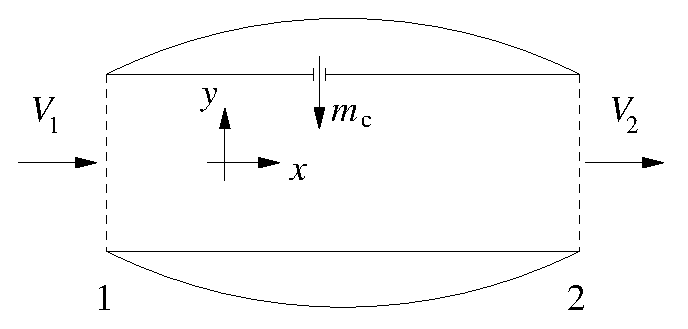
\includegraphics[width=0.90\textwidth]{./fig/motore_a_getto.eps}
   \end{center}
\end{minipage}
\end{tabular}

\sol
\begin{equation}
    T = \rho V_1 A (V_2-V_1) + V_2 \dot{m}_c \ .
\end{equation}

\partone
 Bilanci integrali di massa e quantità di moto.
\begin{equation}
\begin{cases}
  \frac{d}{dt} \int_V \rho = -\oint_{\partial V} \rho \bm{u} \cdot \hat{\bm{n}}  & \text{(massa)} \\
  \frac{d}{dt} \int_V \rho \bm{u} = -\oint_{\partial V} \rho \bm{u} \bm{u} \cdot \hat{\bm{n}}
  +\int_V \bm{f} - \oint_{\partial V} p \hat{\bm{n}} + \oint_{\partial V} \bm{s_n} & \text{(quantità di moto)}
\end{cases}
\end{equation}

\parttwo
Ipotesi: Regime stazionario. Fluido non viscoso (?). Profilo costante di velocità. No gravità.

\begin{itemize}
  \item Scrittura dei bilanci integrali con le semplificazioni opportune, derivanti dalle ipotesi.
    \begin{equation}
     \begin{cases}
      \oint_{\partial V} \rho \bm{u} \cdot \hat{\bm{n}} = 0  & \text{(massa)} \\
      \oint_{\partial V} \rho \bm{u} \bm{u} \cdot \hat{\bm{n}} = \oint_{\partial V} \bm{t_n} & \text{(quantità di moto)}
     \end{cases}
    \end{equation}
  \item Ulteriore semplificazione usando l'ipotesi di profili di velocità uniformi
    \begin{equation}
     \begin{cases}
      - \rho_1 V_1 A_1 -\dot{m}_c + \rho_2 V_2 A_2 = 0  \\
      - \rho_1 \vec{V_1} V_1 A_1 + \rho_2 \vec{V_2} V_2 A_2 - \dot{m}_c \vec{v}_c = \oint_{S1\cup S2\cup S3} \bm{t_n}
     \end{cases}
    \end{equation}
  \item Relazione tra l'integrale della pressione e la risultante delle forze agenti sul gomito, sfruttando il fatto che l'integrale della normale su tutta la superficie è identicamente nullo. Si identificano con $S_1$ la superficie di ingresso, $S_2$ la superficie di uscita, $S_3$ la superficie laterale interna del motore, $S_{3_o}$ la superficie laterale esterna del motore.
    \begin{equation}
     \begin{aligned}
      \displaystyle\oint_{S_1\cup S_2\cup S_3} \bm{t_n} & = \displaystyle\oint_{S_1\cup S_2\cup S_3} \bm{t_n} + \underbrace{\displaystyle\oint_{S_1\cup S_2\cup S{3_o}} p_a \hat{\bm{n}}}_{=0} = \\
      & = -\int_{S_1} (p-p_a) \hat{\bm{n}} - \int_{S_2} (p-p_a) \hat{\bm{n}} + \int_{S_{3_o}} p_a \hat{\bm{n}} + \int_{S_3} \bm{t_n}  = \qquad(p|_{S_1} = p|_{S_2} = p_a) \\
      & = \int_{S_{3_o}} p_a \hat{\bm{n}} + \int_{S_3} \bm{t_n} = \\
      & = \oint_{S_{eng}} \bm{t_n} = - \vec{F}
     \end{aligned}
    \end{equation}
  \item L'equazione della quantità di moto diventa quindi:
  \begin{equation}
  - \rho_1 \vec{V_1} V_1 A_1 + \rho_2 \vec{V_2} V_2 A_2 - \dot{m}_c \vec{v}_c = - \vec{F}
  \end{equation}
  \item Mettendo a sistema l'equazione del bilancio di massa e la proiezione in direzione orizzontale dell'equazione della quantità di moto (si assume che l'iniezione del combustibile, e quindi $\bm{v}_c$, sia perpendicolare all'asse x e quindi non compare nel bilancio della quantità di moto in direzione x):
  \begin{equation}
  \begin{cases}
    \rho_2 V_2 A = \rho_1 V_1 A + \dot{m}_c \\
    -\rho_1 V_1^2 A + \rho_2 V_2^2 A = -F_x 
  \end{cases}
  \end{equation}
  
  Si ottiene
  
  \begin{equation}
  \begin{aligned}
    F_x & = \rho_1 V_1^2 A - \rho_2 V_2^2 A = \\
        & = \rho_1 V_1^2 A - (\rho_2 V_2 A) V_2 = \\
        & = \rho_1 V_1^2 A - V_2 (\rho_1 V_1 A + \dot{m}_c) = \\
        & = \rho_1 V_1 A (V_1 - V_2) - V_2 \dot{m}_c
  \end{aligned}
  \end{equation}

  E la spinta coincide con la componente lungo x appena calcolata:
  \begin{equation}
    T = \rho_1 V_1 A (V_2 - V_1) + V_2 \dot{m}_c
  \end{equation}
  
  La spinta risulta quindi: $T = -F_x = 38374N$.
  
  \vspace{0.3cm}
  \textit{Interpretazione dei risultati e osservazioni.} 

In prima approssimazione, la spinta in un motore a getto è una funzione della portata d'aria e della differenza di velocità tra ingresso e uscita. Spesso in molte applicazioni il termine $\dot{m}_c$ è trascurabile.

Ragionare in questo caso sulla validità dell'approssimazione $\bm{t_n} = -p\bm{\hat{n}}$ nella 
definizione della risultante delle forze sul motore.


  
\end{itemize}
 % motore a getto (1)
\newpage
\noindent
\begin{tabular}{cc}
\begin{minipage}{0.60\textwidth}
\begin{exerciseS}[Gomito]
Un condotto di sezione circolare avente diametro $D = 5\ cm$ 
forma un gomito con angolo di $90^\circ$. Nel condotto scorre acqua ($\rho = 
999\ kg/m^3$) in regime stazionario con velocità $V = 
0.5\ rm m/s$. All'esterno del condotto vi è atmosfera con 
pressione uniforme $P_{atm}=101325\ Pa$; inoltre le pressioni 
all'ingresso e all'uscita del gomito sono uniformi sulla sezione ed 
entrambe pari a $P=10^6\ Pa$. Calcolare la forza $\bm{F}$ agente 
sul gomito.\\
($\bm{F} = -1765.03\hat{\bm{x}} + 1765.03\hat{\bm{y}}\  N$)
\end{exerciseS}
\end{minipage}
&
\begin{minipage}{0.35\textwidth}
   \begin{center}
   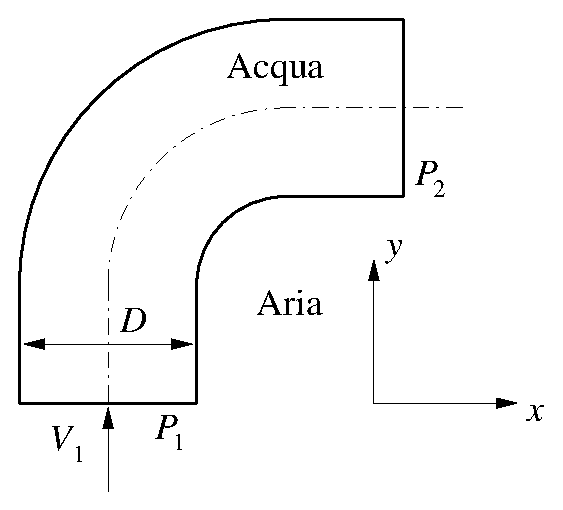
\includegraphics[width=0.70\textwidth]{./fig/gomito_01.eps}
   \end{center}
\end{minipage}
\end{tabular}


\sol

\partone
 Bilanci integrali di massa e quantità di moto. ...
\begin{equation}
\begin{cases}
  \frac{d}{dt} \int_V \rho = -\oint_{\partial V} \rho \bm{u} \cdot \hat{\bm{n}}  & \text{(massa)} \\
  \frac{d}{dt} \int_V \rho \bm{u} = -\oint_{\partial V} \rho \bm{u} \bm{u} \cdot \hat{\bm{n}}
  +\int_V \bm{F} - \oint_{\partial V} p \hat{\bm{n}} + \oint_{\partial V} {\bm{s_n}} & \text{(quantità di moto)}
\end{cases}
\end{equation}

\parttwo
Vengono fatte alcune ipotesi: regime stazionario, fluido incomprimibile, fluido non viscoso, profili costanti di velocità, no gravità.
Si scrivono i bilanci integrali semplificati, si riconoscono in essi e si calcolano le azioni scambiate con il corpo.

\begin{itemize}
  \item Scrittura dei bilanci integrali opportunamente semplificati (ipotesi).
    \begin{equation}
     \begin{cases}
      \oint_{\partial V} \rho \bm{u} \cdot \hat{\bm{n}} = 0  & \text{(massa)} \\
      \oint_{\partial V} \rho \bm{u} \bm{u} \cdot \hat{\bm{n}} = \oint_{\partial V} \bm{t_n} & \text{(quantità di moto)}
     \end{cases}
    \end{equation}
  \item Ulteriore semplificazione usando l'ipotesi di densità costante e profili di velocità uniformi
    \begin{equation}
     \begin{cases}
      -V_1 A_1 + V_2 A_2 = 0 \qquad \qquad \qquad \Rightarrow  V_1 = V_2 = V \\
      - \rho \vec{V_1} V_1 A_1 + \rho \vec{V_2} V_2 A_2 = \oint_{\partial V} \bm{t_n}
     \end{cases}
    \end{equation}
  \item Relazione tra l'integrale degli sforzi sulla superficie e la risultante delle forze agenti sul gomito, sfruttando il fatto che l'integrale della normale su tutta la superficie è identicamente nullo. Si identificano con $S_1$ la superficie di ingresso, $S_2$ la superficie di uscita, $S_3$ la superficie laterale.
    \begin{equation}
     \begin{aligned}
       \displaystyle\oint_{S_1\cup S_2\cup S_3} \bm{t_n} & =  \displaystyle\oint_{S_1\cup S_2\cup S_3} \bm{t_n} + \underbrace{\displaystyle\oint_{S_1\cup S_2\cup S_3} p_a \hat{n}}_{=0} = \\
      & = -\oint_{S_1} (p-p_a) \hat{n} - \oint_{S_2} (p-p_a) \hat{n} + \underbrace{\oint_{S_3} (\bm{t_n}+p_a \hat{n})}_{=-\bm{F}} =  \\
      & = -\oint_{S_1} (p-p_a) \hat{n} - \oint_{S_2} (p-p_a) \hat{n} - \bm{F} 
     \end{aligned}
    \end{equation}
  \item Proiezione lungo i due assi del sistema di riferimento della risultante delle forze agenti sul gomito (dopo averla inserita nell'equazione di bilancio della quantità di moto)
\begin{equation}
  \begin{cases}
    F_x = - \rho V^2 A - (p_2 - p_a)A   \\
    F_y =  \rho V^2 A + (p_1 - p_a)A  
  \end{cases}
  \end{equation}
%  \begin{equation}
%  \begin{cases}
%    F_x = - \rho V^2 A - (p_2 - p_a)A & \quad \Rightarrow \quad   F_x = -1765.03 N  \\
%    F_y =  \rho V^2 A + (p_1 - p_a)A  & \quad \Rightarrow \quad   F_y =  1765.03 N
%  \end{cases}
%  \end{equation}
\end{itemize}
 % gomito (1)
\newpage

\noindent
\begin{tabular}{cc}
\begin{minipage}{0.60\textwidth}
\begin{exerciseS}[Gomito]
Si consideri la corrente stazionaria nel gomito a 90$\,^\circ$ di una 
galleria a vento a circuito chiuso di cui è mostrata in figura la 
sezione nel piano $x$--$y$. Siano assegnate le aree della sezione di 
ingresso, $S_1 = 16 \ m^2$, e di uscita, $S_2 = 56 \ m^2$, 
la portata in volume $Q_1 = 1600 \  m^3/s$ e le pressioni nella 
sezione di ingresso, $P_1 = 1.05 \ bar$, e nella sezione di uscita, 
$P_2 = 1.106 \  bar$. Assumendo che il flusso d'aria sia incomprimibile 
($\rho = 1.225\ kg/m^3$) e che la velocità sulle sezioni di ingresso 
e uscita possa ritenersi uniforme, si determinino le componenti $F_x$ ed 
$F_y$ della spinta che esso esercita sul gomito, usando la convenzione 
indicata in figura.\\
($F_x = 1.876\,10^6\ N$, $F_y = -6.251\,10^6\ N$)
\end{exerciseS}
\end{minipage}
&
\begin{minipage}{0.35\textwidth}
   \begin{center}
   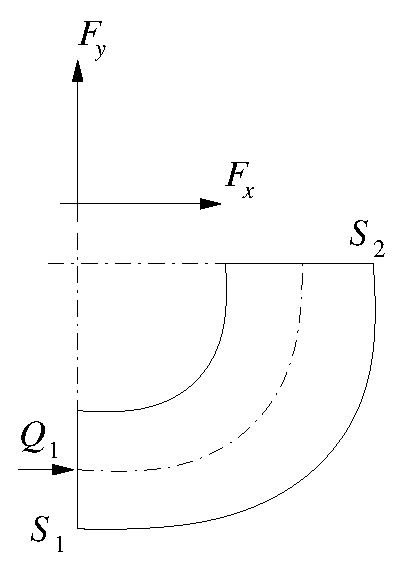
\includegraphics[width=0.60\textwidth]{./fig/gomito_galleria.eps}
   \end{center}
\end{minipage}
\end{tabular}


%%%%%%%%%%%%%%%%%%%%%%%%%%%%%%%%%%%%%%%%%%%%%%%%%%%%%%%%%%%%%%%%%%

\sol

\partone
  Bilanci integrali di massa e quantità di moto.
\begin{equation}
\begin{cases}
  \frac{d}{dt} \int_V \rho = -\oint_{\partial V} \rho \bm{u} \cdot \hat{\bm{n}}  & \text{(massa)} \\
  \frac{d}{dt} \int_V \rho \bm{u} = -\oint_{\partial V} \rho \bm{u} \bm{u} \cdot \hat{\bm{n}}
  +\int_V \bm{f} - \oint_{\partial V} p \hat{\bm{n}} + \oint_{\partial V} {\bm{t}_s} & \text{(quantità di moto)}
\end{cases}
\end{equation}



\parttwo
Vengono fatte alcune ipotesi: regime stazionario, fluido incomprimibile, fluido non viscoso, profili costanti di velocità, no gravità.
Si scrivono i bilanci integrali semplificati, si riconoscono in essi e si calcolano le azioni scambiate con il corpo.

\begin{itemize}
  \item Scrittura dei bilanci integrali con le semplificazioni opportune, derivanti dalle ipotesi.
    \begin{equation}
     \begin{cases}
      \oint_{\partial V} \rho \bm{u} \cdot \hat{\bm{n}} = 0  & \text{(massa)} \\
      \oint_{\partial V} \rho \bm{u} \bm{u} \cdot \hat{\bm{n}} = \oint_{\partial V} \bm{t_n} & \text{(quantità di moto)}
     \end{cases}
    \end{equation}
  \item Ulteriore semplificazione usando l'ipotesi di densità costante e profili di velocità uniformi
    \begin{equation}
     \begin{cases}
      -V_1 A_1 + V_2 A_2 = 0  & \quad \Rightarrow \quad V_1 A_1 = V_2 A_2 = Q \\
      - \rho \vec{V_1} V_1 A_1 + \rho \vec{V_2} V_2 A_2 = \oint_{\partial V} \bm{t_n}
     \end{cases}
    \end{equation}
  \item Relazione tra l'integrale della pressione e la risultante delle forze agenti sul gomito, sfruttando il fatto che l'integrale della normale su tutta la superficie è identicamente nullo. Si identificano con $S_1$ la superficie di ingresso, $S_2$ la superficie di uscita, $S_3$ la superficie laterale.
    \begin{equation}
     \begin{aligned}
      \displaystyle\oint_{S_1\cup S_2\cup S_3} p \hat{n} & =  \displaystyle\oint_{S_1\cup S_2\cup S_3} \bm{t_n} + \displaystyle\oint_{S_1\cup S_2\cup S_3} p_a \hat{n} = \\
      & = -\oint_{S_1} (p-p_a) \hat{n} - \oint_{S_2} (p-p_a) \hat{n} + \underbrace{\oint_{S_3} (\bm{t_n}+p_a\hat{n})}_{=-\bm{f}}  =  \\
      & = -\oint_{S_1} (p-p_a) \hat{n} - \oint_{S_2} (p-p_a) \hat{n} - \bm{f}
     \end{aligned}
    \end{equation}
  \item L'equazione della quantità di moto diventa quindi:
  \begin{equation}
  - \rho \bm{V_1} V_1 A_1 + \rho \bm{V_2} V_2 A_2 = - (p_1 - p_a) A_1 \hat{n}_1 - (p_2 - p_a) A_2 \hat{n}_2 - \bm{F}
  \end{equation}
  \item Proiezione lungo i due assi del sistema di riferimento della risultante delle forze agenti sul gomito.
  Se si considera $p_a = 0$, i risultati numerici sono i seguenti:
  \begin{equation}
  \begin{cases}
    F_x = \rho \frac{Q^2}{A_1} + (p_1 - p_a)A_1  & \quad \Rightarrow \quad   F_x = 1.876 \cdot 10^6 N  \\
    F_y = -  \rho \frac{Q^2}{A_2} - (p_2 - p_a)A_2  & \quad \Rightarrow \quad   F_y =-6.250 \cdot 10^6 N
  \end{cases}
  \end{equation}
\end{itemize}

 % gomito (2)

% todo: write the solution?
\newpage
\noindent
\begin{tabular}{cc}
\begin{minipage}{0.45\textwidth}
\begin{exerciseS}[Profili in schiera]
Un numero elevato di profili è disposto come in figura. Il profilo di ingresso
è uniforme $\bm{u} = U_\infty \bm{\hat{x}}$, mentre il profilo di uscita ha andamento
$\bm{u} = \beta U_\infty (\cos \theta \bm{\hat{x}} - \sin \theta \bm{\hat{y}})
\sin{\frac{\pi \eta}{H}}$ in ogni canale (sia $\eta$ la coordinata che descrive la
sezione di uscita).
Sulla sezione di ingresso la pressione media vale $P_1$, sulla sezione di uscita
 $P_2$. 

Calcolare il fattore $\beta$ del profilo di velocità in uscita e la risultante delle
 forze (per unità di apertura) agente sul singolo profilo.

(Risultati: $\beta = \frac{\pi}{2 \cos \theta}, \bm{F} = [(P_1 - P_2) H + \rho U^2 H ((1-\pi^2/8) ]\bm{\hat{x}} + \pi^2/8 \tan \theta \bm{\hat{y}}) $)
\end{exerciseS}
\end{minipage}
&
\begin{minipage}{0.50\textwidth}
   \begin{center}
   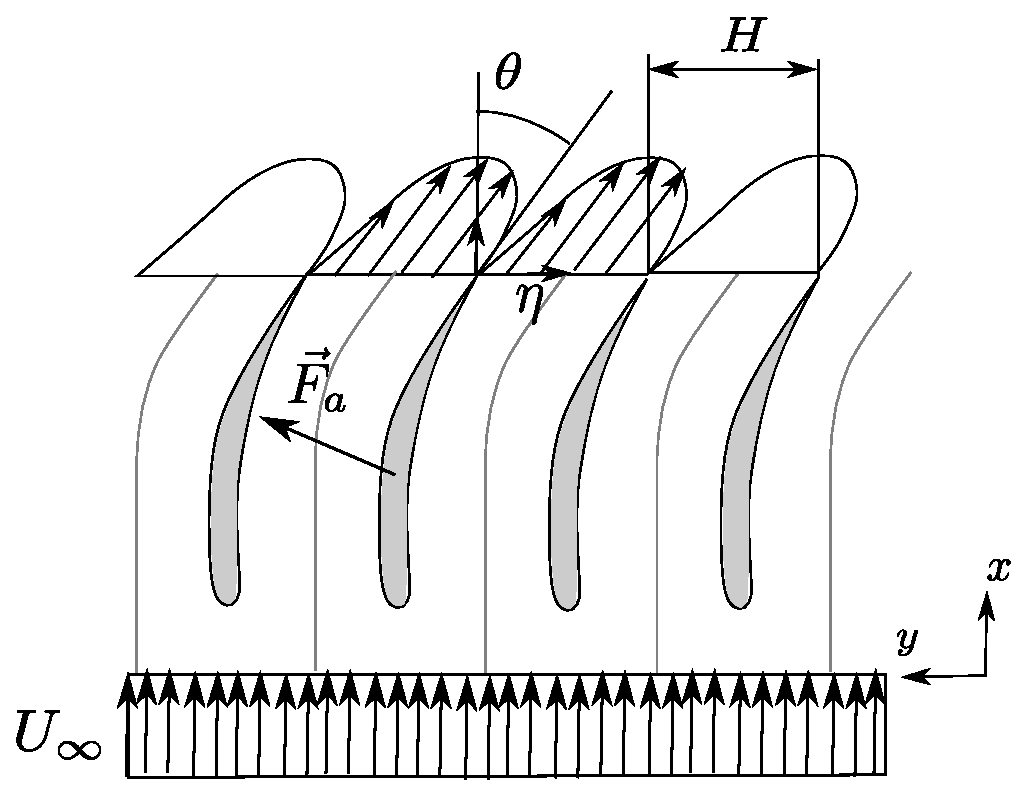
\includegraphics[width=0.95\textwidth]{./fig/wings.eps}
   \end{center}
\end{minipage}
\end{tabular}

\vspace{1.0cm}

\sol

\partone
  Bilanci integrali di massa e quantità di moto. Equazioni di equilibrio (equazioni fondamentali della dinamica classica). Principio di azione e reazione. Integrale della normale su una superficie chiusa è identicamente nullo. Simmetria.
\begin{itemize}
  \item Ricavare il coefficiente $\beta$ dal bilancio di massa
  \item Usare le ipotesi di simmetria nel bilancio di quantità di moto per annullare alcuni termini
\end{itemize} 

\parttwo

Si ricava il coefficiente $\beta$ dal bilancio di massa in forma integrale. Si utilizza la simmetria del problema nel bilancio di quantità moto per
 ricavare le azioni sui profili.

 % profili in schiera	

\newpage
\noindent
\begin{tabular}{cc}
\begin{minipage}{0.60\textwidth}
\begin{exerciseS}[Difetto di scia: stima resistenza]
Calcolare la resistenza di un profilo immerso in una corrente stazionaria 
con velocità asintotica ${\bm{V}}_\infty$, sapendo la distribuzione della 
componente di velocità $u(y)$ parallela a ${\bm{V}}_\infty$ a valle del 
profilo e assumendo che:
\begin{itemize}
\item la pressione statica sul contorno del volume di controllo
      sia costante e pari a quella della corrente indisturbata a monte
      del profilo;
\item sul lato superiore e inferiore del volume di controllo
      sia possibile trascurare la componente lungo l'asse $x$ della 
      perturbazione della velocit\`a dovuta alla presenza del profilo:
      $
      \bm{V} = (V_{\infty}+u,v) \simeq (V_{\infty},v).
      $
\end{itemize}
($R = \int_0^{ H}\rho \, u(y) [V_{\infty}-u(y)] dy.$)
\end{exerciseS}
\end{minipage}
&
\begin{minipage}{0.35\textwidth}
   \begin{center}
   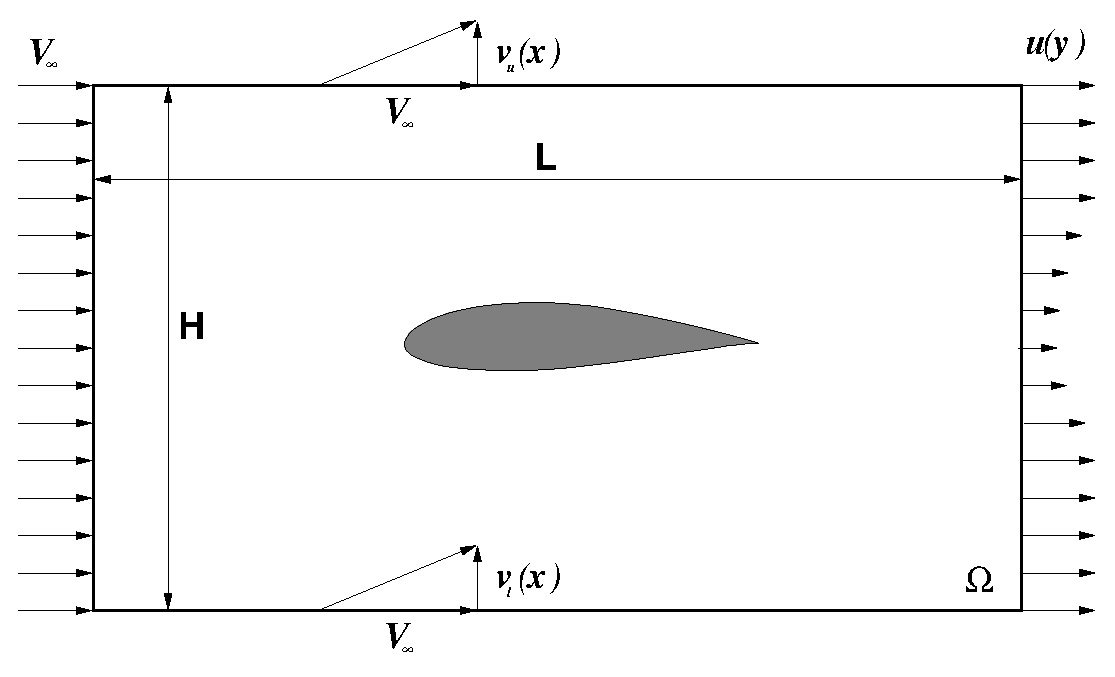
\includegraphics[width=0.90\textwidth]{./fig/airfoil.eps}
   \end{center}
\end{minipage}
\end{tabular}

\vspace{1.0cm}

\sol

\partone
  Bilanci integrali di massa e quantità di moto. Equazioni di equilibrio (equazioni fondamentali della dinamica classica). Principio di azione e reazione. Integrale della normale su una superficie chiusa è identicamente nullo. Esperienza in laboratorio sul \textit{difetto di scia}.

\parttwo
 Vengono scritti i bilanci integrali di massa e quantità di moto, opportunamente semplificati (ipotesi di stazionarietà $\frac{d}{dt} \equiv 0$, densità costante $\rho = \bar{\rho}$, ipotesi sulle condizioni sul bordo esterno del dominio); all'interno dei bilanci si possono riconoscere i termini legati alle azioni scambiate dal fluido con il profilo
 (l'incognita del problema); si sfrutta infine la geometria rettangolare del contorno esterno e le ipotesi su di esso per ottenere una forma ulteriormente semplificata dei bilanci e trovare la soluzione del problema.

\begin{itemize}
  \item Scrittura e semplificazione dei bilanci di massa e quantità di moto.
    \begin{equation}
      \begin{cases}
       \frac{d}{d t} \int_{\Omega} \rho + \oint_{\partial \Omega} \rho \bm{u} \cdot \hat{\bm{n}} = 0 & \qquad \text{(massa)} \\
       \frac{d}{d t} \int_{\Omega} \rho \bm{u} + \oint_{\partial \Omega} \rho \bm{u} \bm{u} \cdot \hat{\bm{n}} +
        \oint_{\partial \Omega} p \hat{\bm{n}} - \oint_{\partial \Omega} \bm{s_n} = 0  
        & \qquad \text{(quantità di moto)}  %\Rb^{ext}
      \end{cases}
    \end{equation}

%Dove $\Rb^{ext}$ è la risultante delle forze esterne che agiscono sul fluido. Nell'ipotesi che non ci siano altre forze esterne agenti sul fluido, se non quelle prodotte dal profilo, la forza $\bm{F}$ esercitata dal fluido sul profilo sarà uguale e contraria a $\Rb^{ext}$. L'incognita del problema è la resistenza del profilo, cioè la componente di $\bm{F}$ nella direzione della velocità asintotica $\Vb_{\infty}$ (in questo caso $F_x$).

Nel problema, il controno del dominio fluido $\partial \Omega$ è costituito dal bordo rettangolare $\gamma_\infty$ lontano dal profilo e dal bordo $\gamma_p$ coincidente con il profilo stesso. La forza $\bm{F}$ agente sul profilo è l'integrale degli sforzi generati dal fluido (uguali e contrari agli sforzi agenti sul fluido) sul contorno del profilo. Inoltre si può fare l'ipotesi di sforzi viscosi nulli e pressione costante sul bordo esterno: l'integrale sul dominio esterno si riduce all'integrale della normale su una superficie chiusa ed è quindi nullo. Si può dunque scrivere:
\begin{equation}
 \oint_{\partial \Omega} (-p \hat{\bm{n}} + \bm{s_n}) = \oint_{\partial \Omega} \bm{t_n} = \underbrace{\oint_{\gamma_p} \bm{t_n}}_{=-\bm{F}} + \underbrace{\oint_{\gamma_\infty} \bm{t_n}}_{=0} = -\bm{F}
\end{equation}

\textit{Osservazione. A differenza di quanto fatto in classe, non
è stata fatta l'ipotesi di fluido non viscoso; il contributo 
all'infinito si annulla con l'ipotesi di pressione costante 
all'infinito e sforzi viscosi trascurabili. Per ritrovarsi con gli appunti, sostituire $\bm{t_n}$ con
$-p\bm{\hat{n}}$}.

Dopo aver fatto l'ipotesi di stazionarietà e aver inserito la definizione di $\bm{F}$ appena data, le equazioni di bilancio possono essere scritte come:
    \begin{equation}
      \begin{cases}
      & \oint_{\partial \Omega} \rho \bm{u} \cdot \hat{\bm{n}} = 0  \\
      & \bm{F} = - \oint_{\partial \Omega} \rho \bm{u} \bm{u} \cdot \hat{\bm{n}} 
      \end{cases}
    \label{eqn:airfoil_bil_int}
    \end{equation}

Il bilancio di quantità di moto può essere scritto esplicitando e
separando le componenti vettoriali.
    \begin{equation}
    \begin{aligned}
       F_x\bm{\hat{x}} + F_y\bm{\hat{y}} 
& = - \oint_{\partial \Omega} \rho (u \bm{x} + v \bm{y}) \bm{u} \cdot \hat{\bm{n}} \\
& =       - \bm{\hat{x}} \oint_{\partial \Omega} \rho u \bm{u} \cdot \hat{\bm{n}} -  \bm{\hat{y}} \oint_{\partial \Omega} \rho v  \bm{u} \cdot \hat{\bm{n}}
    \end{aligned}
    \end{equation}
\item Scrittura delle equazioni di bilancio in componenti (sfruttando la geometria rettangolare del bordo esterno: $\gamma_1$ indica il bordo di sinistra, $\gamma_2$ il bordo inferiore, $\gamma_3$ quello di destra, $\gamma_4$ quello superiore).

\textit{Attenzione: la normale è quella uscente dal dominio fluido. Sul contorno del profilo, la
normale è entrante nel profilo. 
In più: non fare confusione tra azioni del profilo agenti sul fluido e azioni del fluido agenti 
sul profilo!}
  \begin{equation}
     \begin{cases}
      & 0 = \oint_{\partial \Omega} \rho \bm{u} \cdot \hat{\bm{n}} = -\int_{\gamma_1} \rho u
      -\int_{\gamma_2} \rho v +\int_{\gamma_3} \rho u +\int_{\gamma_4} \rho v \\
      & F_x = +\int_{\gamma_1} \rho u^2 +\int_{\gamma_2} \rho u v -\int_{\gamma_3} \rho u^2 -\int_{\gamma_4} \rho u v \\
      & F_y = +\int_{\gamma_1} \rho u v +\int_{\gamma_2} \rho v^2 -\int_{\gamma_3} \rho u v -\int_{\gamma_4} \rho v^2
     \end{cases}
  \end{equation}

\item Ipotesi sulla velocità sui lati orizzontali ($u|_{\gamma_2} = u|_{\gamma_4} = V_\infty$ costante), per poter ulteriormente semplificare il risultato.
   \begin{equation}
     \begin{cases}
        \int_{\gamma_2} \rho v  -\int_{\gamma_4} \rho v = -\int_{\gamma_1} \rho u+\int_{\gamma_3} \rho u\\
       F_x = +\int_{\gamma_1} \rho u^2 -\int_{\gamma_3} \rho u^2 + V_\infty \left[ \int_{\gamma_2} \rho v  -\int_{\gamma_4} \rho v \right]
     \end{cases}
  \end{equation}
E inserendo la prima nella seconda:
\begin{equation}
  \begin{aligned}
       F_x  & = \int_{\gamma_1} \rho u^2 -\int_{\gamma_3} \rho u^2 + V_\infty \left[-\int_{\gamma_1} \rho u+\int_{\gamma_3} \rho u \right] = \\
       & = \int_{\gamma_1} \rho u (u-V_\infty) + \int_{\gamma_3} \rho u (V_\infty-u) = \quad \text{($u|_{\gamma_1} = V_\infty  \Rightarrow $ il primo integrale è nullo)} \\
       & = \int_{\gamma_3} \rho u (V_\infty-u) = \\
       & = \int_{0}^{H} \rho u(y) (V_\infty - u(y)) dy
  \end{aligned}
\label{eqn:difetto_scia}
\end{equation}

\end{itemize}

\noindent
\textbf{Osservazioni.} Tramite la misura del campo di velocità in
galleria è possibile stimare la resistenza del corpo.
Le condizioni di ``aria libera'' e in galleria sono diverse. In generale, in galleria il fluido è confinato dalle pareti di galleria, maggiormente ``vincolato''. Inoltre sulle pareti della galleria esiste una condizione di adesione, $\bm{u}=\bm{0}$: per la conservazione della massa, il rallentamento del fluido in corrispondenza delle pareti della galleria viene compensato da un incremento della velocità nella regione ``più lontana'' dalla parete, rispetto a un corpo in aria libera.
 Per tenere conto di effetti di 
\textbf{bloccaggio} dovuti al confinamento in galleria, è necessario compiere delle correzioni delle misure sperimentali.
Agli effetti di bloccaggio, vanno aggiunti gli effetti di \textbf{galleggiamento} dovuti al gradiente di pressione lungo la galleria, che danno un effetto di resistenza aggiuntiva.
Inoltre è importante che la dimensione del corpo rispetto alla dimensione della galleria non sia né ``troppo grosso'' (per problemi di 'bloccaggio'), né, di solito, ``troppo piccolo'' (per motivi di similitudine; ma sarà argomento di puntate successive del corso...). \'E importante avere in mente la necessità di prestare attenzione a questi aspetti, quando vengono svolte attività sperimentali. Ma questo sarà argomento di altri capitoli o di altri corsi...


 % difetto di scia
% Stima resistenza (replica esperimento in galleria)
\subsection{Attività sperimentale: difetto di scia e volume di controllo.}

L'esercizio svolto in precedenza risulta propedeutico per l'analisi dei dati ottenuti tramite alcune attività sperimentali, per ottenere delle risultanti di forze e momenti da misure del campo di velocità (e pressione, a volte) tramite i bilanci integrali.
Le attività svolte nel mondo reale sono affette da imprecisioni e incertezze. La quantificazione (o almeno la stima) dell'incertezza del risultato di un'attività sperimentale è parte integrante del risultato stesso. 
I valori $x_i, \ i=1:N$ di grandezze misurate possono essere combinati per calcolare delle grandezze derivate $f(x_i)$. I \textit{datasheet} che accompagnano uno strumento raccolgono anche le informazioni sulla sua incertezza di misura, spesso in forma di intervallo di confidenza o di scarto quadratico medio. L'incertezza sulle misure sperimentali $x_i$ si propaga sul valore della funzione $f(x_i)$. Nell'ipotesi che le incertezze di misura sulle variabili $d_i$ siano tra di loro indipendenti e non correlate, è possibile utilizzare la \textbf{formula RSS} (\textbf{root-sum-squares}) per la propagazione dell'incertezza. Se la misura $x_i$ ha incertezza $\sigma_{x_i}$, una stima dell'incertezza su $f$ vale
\begin{equation}
  \sigma_f^2 = \sum_{i=1}^{N} \left( \dfrac{\partial f}{\partial x_i} \right)^2 \sigma_{x_i}^2 \ .
\end{equation}
%
L'incertezza $\sigma^2_f$ sulla quantità $f$, obiettivo dell'attività sperimentale, è un indicatore della bontà del metodo sperimentale utilizzato ed del sistema di miusra disponibile per tale attività. In generale, l'incertezza sulla grandezza desiderata deve essere ``molto minore'' della grandezza stessa: in caso contrario, l'apparato sperimentale risulterebbe indeguato all'esperimento.
Essendo parte integrante del risultato, è buona regola indicare l'incertezza sui risultati delle attività sperimentali, ad esempio fornendone il valore numerico, il valore relativo alla misura o gli intervalli di confidenza sui grafici.

% \paragraph{Difetto di scia e resistenza del profilo.}
% \'E possibile stimare la resistenza di un profilo a partire dalla misura del difetto di scia.
%  La misura di velocità in scia viene effettuata (con una sonda di Pitot o altro \dots)
%  in punti discreti, più radi lontano dalla scia del profilo,
%  fiù fitti in corrispondenza della scia dove i gradienti sono maggiori.
% L'integrale nella formula (\ref{eqn:difetto_scia}) viene approssimato con un metodo numerico,
%  come ad esempio la formula del punto medio, quella del trapezio, \dots
% Utilizzando qui per semplicità la formula del punto medio, è possibile scrivere
% \begin{equation}
%  F_x = \int_{0}^{H} \rho u(y) (U_\infty - u(y)) dy
%     \approx \sum_{k=1}^{N} \rho \left[ u_k (U_\infty - u_k) \right] \Delta s_k
% \end{equation}
% Le misure ottenute dalla sonda sono affette da incertezza $\sigma_{u_i}$; la derivata $\partial F_x / \partial u_i$ è
% \begin{equation}
%  \dfrac{\partial F_x}{\partial u_m}  = \rho \left( U_\infty - 2 u_m \right) \Delta s_m
% \end{equation}
% La stima dell'incertezza sulla resistenza è quindi
% \begin{equation}
%  \sigma_{F_x}^2 = \sum_{i=1}^{N} \left[ \rho \left( U_\infty - 2 u_i \right) \Delta s_i \right]^2 \sigma_{u_i}^2
% \end{equation}
% 

\paragraph{Risultante delle forze: bilancio di quantità di moto di un volume di controllo .}
Esistono metodi sperimentali, come ad esempio la \textbf{PIV} (Particle Image Velocimetry o, in italiano, velocimetria a immagini di particelle), che permettono di ottenere il campo di velocità in un determinato istante all'interno di un dominio di misura, un piano bidimensionale o un volume tridimensionale.
Il bilancio di quantità di moto del volume di controllo contenente un corpo solido permette poi di calcolare la risultante delle forze scambiate tra corpo e fluido.

\noindent
 Per semplicità, viene considerato un campo di moto bidimensionale, $\bm{u}(x,y)=u(x,y)\bm{\hat{x}}+v(x,y)\bm{\hat{y}}$. Ad esempio, il campo di moto attorno alla mezzeria di un'ala allungata senza freccia investita da una corrente con un angolo di incidenza ridotto è in buona approssimazione bidimensionale.
 In questo caso, misure PIV (PIV-2D-2C) forniscono le due componenti (2C) del campo di velocità nel piano (2D) di misura. Tramite il bilancio della quantità di moto del dominio bidimensionale, è possibile ottenere una stima della risultante delle forze (per unità di apertura) che esercita il fluido sul profilo di ala tagliato dal piano di misura.
Considerando gli effetti viscosi trascurabili, al di fuori di regioni di dimensione ridotta nell'ambito di applicazioni aeronautiche (alto numero di Reynolds, strato limite e scie sottili), il bilancio integrale della quantità di moto del fluido nel volume di misura fornisce, in un caso stazionario, la risultante delle forze ${\bm{R}}$ agenti sul corpo, 
\begin{equation}
 \bm{R} = -\oint_S \rho \bm{u} \bm{u} \cdot \bm{\hat{n}} - \oint_S p \bm{\hat{n}} \ ,
\end{equation}
avendo trascurato il contributo delle forze di volume.
%
Nell'ipotesi, più che sensata per molte applicazioni aeronautiche, che sia valido il teorema di Bernoulli sulla frontiera $S$ del volume di controllo, la pressione viene espressa in funzione della velocità locale e dello stato della corrente asintotica,
\begin{equation}
 p = p_\infty + \rho \dfrac{|\bm{U_\infty}|^2}{2} - \rho \dfrac{|\bm{u}|^2}{2} \ .
\end{equation}
Inserendo questa espressione della pressione nell'espressione della risultante delle forze ed eliminando gli integrali (nulli) su una superficie chiusa delle quantità costanti moltiplicate per la normale alla superficie, come ad esempio $\oint_S p_\infty \bm{\hat{n}}$, si può esprimere la risultante $\bm{R}$ della forza aerodinamica agente sul corpo in funzione della sola velocità del fluido sulla frontiera $S$,
\begin{equation}
 \bm{R} = -\oint_S \rho \bm{u} \bm{u} \cdot \bm{\hat{n}} + \oint_S \rho \dfrac{|\bm{u}|^2}{2} \bm{\hat{n}} \ .
\end{equation}
Sotto queste ipotesi, la forza aerodinamica agente sul corpo, in questo esempio l'obiettivo della misura, è stata scritta unicamente come funzione del campo di velocità sulla superficie $S$, fornito come ``risultato diretto'' dell'attività seprimentale. Per semplicità, la densità del fluido viene considerata costante e nota senza incertezza: nel caso che anche il campo di densità fosse affetto da incertezza, la formula RSS permette di aggiungere abbastanza facilmente il suo effetto a quello dovuto all'incertezza sulla misura del campo di velocità.
\newline
% TODO: è possible applicare diversi metodi per ricavare un'approssimazione della risultante e della sua incertezza, partendo da dati discreti...
\paragraph{Risultante delle forze: discretizzazione.}
Per la sua natura, la PIV fornisce dei risultati discreti (non continui): di solito, il campo di velocità viene misurato sui nodi di una griglia cartesiana. Per il calcolo della risultante $\bm{R}$ sono necessari solamente gli $N_n$ nodi esterni $\bm{x_i}, \ i=1:N_n$, posti sul contorno della griglia.
% TODO ...
\newline
Il campo di velocità viene approssimato (linearmente, per semplicità) utilizzando un approccio simile a quello impiegato nella modellazione numerica a elementi finiti. Viene introdotto un insieme completo di funzioni di base $\phi_i(\bm{x}), \ i=1:N_{n}$, lineari a tratti sul contorno $S$, grazie alle quali è possibile scrivere l'approssimazione $\bm{u}^h$ del campo di velocità
\begin{equation}\label{exp:u:fem-exp}
 \bm{u}(\bm{x}) \approx \bm{u}^h(\bm{x}) = \displaystyle\sum_{i=1}^{N_n} \phi_i(\bm{x}) \bm{U_i} \ . 
\end{equation}
Utilizzando funzioni di base lagrangiane, per le quali il valore della funzione $i$-esima $\phi_i(\bm{x})$ è uguale a uno sul nodo $i$-esimo $\bm{x}_i$ e zero sugli altri nodi,
\begin{equation}
 \phi_i(\bm{x_j}) = \delta_{ij} \qquad , \qquad \displaystyle\sum_{i=1}^{N_n} \phi_i(\bm{x}) = 1  \ , \forall i=1:N_n \ ,
\end{equation}
i coefficienti $\bm{U_i}$ della (\ref{exp:u:fem-exp}) concidono con i valori nodali, $\bm{U_i}:=\bm{u}(\bm{x_i})$ ricavati nei punti $\bm{x_i}$ tramite la misura sperimentale. Introducendo il campo di velocità approssimato $\bm{u}^h(\bm{x})$ nell'espressione della risultante delle forze, si ottiene una formula nella quale compaiono gli integrali di superficie del prodotto delle funzioni di base e del versore normale, 
\begin{equation}\label{eqn:RU}
\begin{aligned}
 \bm{R} \approx \bm{R}^h & = -\oint_S \rho \bm{u}^h \bm{u}^h \cdot \bm{\hat{n}} + \oint_S \rho \dfrac{\bm{u}^h \cdot \bm{u}^h}{2} \bm{\hat{n}} = \\
 & = - \rho \sum_{i=1}^{N_n} \sum_{j=1}^{N_n} \bm{U}_i \bm{U}_j \cdot \oint_S \phi_i(\bm{x}) \phi_j(\bm{x}) \bm{\hat{n}}(\bm{x})  + \dfrac{1}{2} \rho \sum_{i=1}^{N_n} \sum_{j=1}^{N_n}\bm{U}_i \cdot \bm{U}_j \oint_S  \phi_i(\bm{x}) \phi_j(\bm{x}) \bm{\hat{n}}(\bm{x}) = \\ 
 & = - \rho \sum_{i=1}^{N_n} \sum_{j=1}^{N_n} \bm{U}_i \bm{U}_j \cdot \bm{I}_{ij}  + \dfrac{1}{2} \rho \sum_{i=1}^{N_n} \sum_{j=1}^{N_n}\bm{U}_i \cdot \bm{U}_j \bm{I}_{ij} \ , 
\end{aligned}
\end{equation}
dove sono stati introdotti i vettori $\bm{I}_{ij} = \oint_S  \phi_i(\bm{x}) \phi_j(\bm{x}) \bm{\hat{n}}(\bm{x})$, facilmente calcolabili in maniera analitica, come spiegato nella sezione \S\ref{sec:fem}. \newline

% -------
\paragraph{Sensitività della risultante al campo di velocità.}
Per ricavare tramite la formula RSS l'incertezza sulla misura della risultante delle forze $\bm{R}$ dall'incertezza sulle misure del campo di velocità $\bm{u}(\bm{x})$, è necessario calcolare la \textit{variazione} di $\bm{R}$ rispetto al campo $\bm{u}(\bm{x})$. Perturbando il campo di velocità $\bm{u}(\bm{x})$ con la variazione $\delta \bm{u}(\bm{x})$, e trascurando i termini di ordine superiore al primo, dopo aver sottratto l'equazione ``non perturbata'', si ottiene la perturbazione della risultante delle forze $\delta \bm{R}$,
\begin{equation}\label{eqn:sens:cont}
\begin{aligned}
  \bm{R} + \delta \bm{R} & = -\oint_S \rho (\bm{u}+\delta\bm{u}) (\bm{u}+\delta\bm{u}) \cdot \bm{\hat{n}} + \oint_S \dfrac{1}{2}\rho (\bm{u}+\delta\bm{u}) \cdot (\bm{u}+\delta\bm{u}) \bm{\hat{n} } \\
  \rightarrow \delta \bm{R} & = -\oint_S \rho \left[ \bm{u} \bm{\hat{n}} \cdot \delta\bm{u} + \bm{u} \cdot \bm{\hat{n}} \delta\bm{u}\right]  + \oint_S \rho \bm{\hat{n}} \bm{u} \cdot \delta\bm{u} \\
 & = \oint_S \rho \left[ - \bm{u} \otimes \bm{\hat{n}} - (\bm{u} \cdot \bm{\hat{n}})\mathbb{I} + \bm{\hat{n}} \otimes \bm{u} \right] \cdot \delta\bm{u} = \\
 & = \oint_S \bm{\nabla}_u \bm{R} \cdot \delta\bm{u} = \\
 & =\oint_S \begin{bmatrix} \nabla_u R_x &  \nabla_v R_x \\ \nabla_u R_y &  \nabla_v R_y  \end{bmatrix} \cdot \begin{bmatrix} \delta u \\ \delta v \end{bmatrix} =
 \oint_S \begin{bmatrix} \bm{\nabla}_{\bm{u}} R_x \cdot \delta \bm{u} \\ \bm{\nabla}_{\bm{u}} R_y \cdot \delta \bm{u} \end{bmatrix} \ ,
\end{aligned}
\end{equation}
avendo introdotto il campo tensoriale della sensitività $\bm{\nabla}_{u} \bm{R}(\bm{x})$ della risultante delle forze rispetto al campo di velocità $\bm{u}(\bm{x})$ ed evidenziato l'influenza delle due componenti del campo di velocità sulle due componenti di forza. L'equazione precedente può essere scritta con notazione indiciale
\begin{equation}
 \qquad \delta R_i = \oint_S \nabla_{u_j} R_i \delta u_j = -\rho \oint_S \left[ u_i n_j + u_k n_k \delta_{ij} - n_i u_j \right] \delta u_j \ ,
\end{equation}
o esplicitamente in coordinate cartesiane, per ricavare l'espressione della sensitività della componenti della forza dalle singole componenti del campo di velocità,
\begin{equation}\label{eqn:sens:cart:simple}
\begin{aligned}
  \qquad & \begin{cases}
  \delta R_x & = \rho \displaystyle\oint_S \left[ -u n_x - u n_x - v n_y + u n_x \right] \delta u + \rho \oint_S \left[ -u n_y + v n_x   \right] \delta v \\
  \delta R_y & = \rho \displaystyle\oint_S \left[ -v n_x + u n_y \right] \delta u + \rho \oint_S \left[ -v n_y - u n_x - v n_y + v n_y \right] \delta v \\
\end{cases}  \vspace{5mm} \\
 \rightarrow & \begin{cases}
 \delta R_x & =
 \rho \displaystyle\oint_S \left[ -u n_x - v n_y \right] \delta u + \rho \oint_S \left[ -u n_y + v n_x   \right] \delta v =
 \oint_S \nabla_{u} R_x \ \delta u + \oint_S \nabla_v R_x \delta v \\
 \delta R_y & = \rho \displaystyle\oint_S \left[ -v n_x + u n_y \right] \delta u + \rho \oint_S \left[ -v n_y - u n_x \right] \delta v =
 \oint_S \nabla_{u} R_y \ \delta u + \oint_S \nabla_v R_y \delta v \ .
\end{cases}
\end{aligned}
\end{equation}

% ------
\paragraph{Sensitività della risultante alle misure di velocità.}
Partendo dall'espansione (\ref{exp:u:fem-exp}) del campo di velocità, la variazione del campo $\bm{u}^h(\bm{x})$ diventa
\begin{equation}\label{exp:du:fem-exp}
 \delta \bm{u}^h(\bm{x}) = \displaystyle\sum_{i=1}^{N_n} \phi_i(\bm{x}) \delta \bm{U}_i \ ,
\end{equation}
avendo indicato con $\delta \bm{U}_i$ la variazione dei valori nodali del campo di velocità. Le funzioni di base sono note, e quindi la loro variazione è nulla.\footnote{L'operazione di variazione ha proprietà simili a quelle di derivazione. Ad esempio la variazione del prodotto di due funzioni vale $\delta(ab) = \delta a \ b + a \ \delta b$.}
%
Introducendo l'espressione (\ref{exp:du:fem-exp}) di $\delta \bm{u}^h(\bm{x})$ all'interno della formula (\ref{eqn:sens:cont}) che lega la variazione $\delta \bm{R}$ alla variazione $\delta \bm{u}(\bm{x})$,
\begin{equation}
 \delta \bm{R} = \oint_S \bm{\nabla}_{\bm{u}} \bm{R} \cdot \delta \bm{u} 
  = \sum_{i=1}^{N_n} \oint_S \phi_i(\bm{x}) \bm{\nabla}_{\bm{u}} \bm{R} \cdot \delta \bm{U}_i  
 = \sum_{i=1}^{N_n} \bm{\nabla}_{\bm{U}_i} \bm{R} \cdot \delta \bm{U}_i \ ,
\end{equation}
 si ricava l'espressione della sensitività $\bm{\nabla}_{\bm{U}_i} \bm{R}$ della risultante delle forze rispetto alla misura di velocità $\bm{U}_i$, in funzione della sensitività $\bm{\nabla}_{\bm{U}_i} \bm{R}(\bm{x})$ della risultante rispetto al campo di velocità $\bm{u}(\bm{x})$ e alle funzioni di base $\phi_i(\bm{x})$,
\begin{equation}
 \bm{\nabla}_{\bm{U}_i} \bm{R} = \oint_S \phi_i(\bm{x}) \bm{\nabla}_{\bm{u}} \bm{R} \ .
\end{equation}
La sensitività $\bm{\nabla}_{\bm{U}_i} R_k$ della componente $R_k$ della risultante delle forze rispetto alla misura $\bm{U}_i$ è quindi
\begin{equation}
 \bm{\nabla}_{\bm{U}_i} R_k 
  = \oint_S \phi_i(\bm{x}) \bm{\nabla}_{\bm{u}} R_k \ . 
\end{equation}


\paragraph{Sensitività della risultante alle misure di velocità: discretizzazione.}
Inserendo l'approssimazione $\bm{u}^h$ nella formula della sensitività $\bm{\nabla}_{\bm{u}} \bm{R}$, è possibile calcolare la sensitività della risultante alle misure di velocità $\bm{U}_i$,
\begin{equation}\label{eqn:sens:RU}
\begin{aligned}
 \bm{\nabla}_{\bm{U}_i} \bm{R} & = \oint_S \phi_i(\bm{x}) \bm{\nabla}_{\bm{u}} \bm{R} =\\
 & = \oint_S \phi_i(\bm{x}) \rho \left[ - \bm{u} \otimes \bm{\hat{n}} - (\bm{u} \cdot \bm{\hat{n}})\mathbb{I} + \bm{\hat{n}} \otimes \bm{u} \right]  = \\
 & = \rho \displaystyle\sum_{j=1}^{N_n} \oint_S \phi_i(\bm{x}) \phi_j(\bm{x}) \left[ - \bm{U}_j \otimes \bm{\hat{n}} - (\bm{U}_j \cdot \bm{\hat{n}})\mathbb{I} + \bm{\hat{n}} \otimes \bm{U}_j \right]  = \\
 & = \rho \displaystyle\sum_{j=1}^{N_n} \left[ - \bm{U}_j \otimes \bm{I}_{ij} - (\bm{U}_j \cdot \bm{I}_{ij})\mathbb{I} + \bm{I}_{ij} \otimes \bm{U}_j \right] \ ,
\end{aligned}
\end{equation}
avendo riconosciuto i vettori $\bm{I}_{ij}$ definiti in precedenza. La sensitività della componente $R_k$ alla misura $\bm{U}_i$ vale
\begin{equation}
 \bm{\nabla}_{\bm{U}_i} R_k =  
  \rho \displaystyle\sum_{j=1}^{N_n} \left[ - U_{j,k} \bm{I}_{ij} - (\bm{U}_j \cdot \bm{I}_{ij}) \bm{\hat{e}}_k + I_{ij,k} \bm{U}_j \right] \ ,
\end{equation}
dove $\bm{\hat{e}}_k$ è il versore in direzione $k$ e $U_{j,k}$, $I_{ij,k}$ le componenti in quella direzione della misura $\bm{U}_i$ e del vettore $\bm{I}_{ij}$.

% {\color{red}
% Si può infine esprimere la sensitività in funzione del campo di velocità. La variazione $\delta \bm{R}$ è
% \begin{equation}
% \begin{aligned}
%  \delta \bm{R} & \approx - \rho \oint_S \left[ \bm{u}^h \bm{\hat{n}} \cdot \delta\bm{u}^h + \bm{u}^h \cdot \bm{\hat{n}}^h \delta\bm{u}\right] + \rho \oint_S \bm{\hat{n}} \bm{u}^h \cdot \delta\bm{u}^h = \\
%  & = - \rho \sum_{i=1}^{N_n} \sum_{j=1}^{N_n} \bm{U}_i \delta \bm{U}_j \cdot \oint_S \phi_i(\bm{x}) \phi_j(\bm{x}) \bm{\hat{n}}(\bm{x}) - \rho \sum_{i=1}^{N_n} \sum_{j=1}^{N_n} \delta\bm{U}_i \bm{U}_j \cdot \oint_S \phi_i(\bm{x}) \phi_j(\bm{x}) \bm{\hat{n}}(\bm{x}) + \\
%  & \hspace{6.7cm} + \rho \sum_{i=1}^{N_n} \sum_{j=1}^{N_n} \delta\bm{U}_i \cdot \bm{U}_j \oint_S  \phi_i(\bm{x}) \phi_j(\bm{x}) \bm{\hat{n}}(\bm{x}) = \\ 
%  & = - \rho \sum_{i=1}^{N_n} \sum_{j=1}^{N_n} \bm{U}_i \delta \bm{U}_j \cdot \bm{I}_{ij}  - \rho \sum_{i=1}^{N_n} \sum_{j=1}^{N_n} \delta \bm{U}_i \bm{U}_j \cdot \bm{I}_{ij} + \sum_{i=1}^{N_n} \sum_{j=1}^{N_n} \delta\bm{U}_i \cdot \bm{U}_j \bm{I}_{ij} \ , 
% \end{aligned}
% \end{equation}
% la cui componente $k$-esima è
% \begin{equation}
%  \delta R_k =  
%   - \rho \sum_{i=1}^{N_n} \sum_{j=1}^{N_n} U_{i,k} \delta \bm{U}_j \cdot \bm{I}_{ij}  - \rho \sum_{i=1}^{N_n} \sum_{j=1}^{N_n} \delta U_{i,k} \bm{U}_j \cdot \bm{I}_{ij} + \sum_{i=1}^{N_n} \sum_{j=1}^{N_n} \delta\bm{U}_i \cdot \bm{U}_j I_{ij,k} \ . 
% \end{equation}
% Sfruttando la simmetria rispetto agli indici dei vettori $\bm{I}_{ij}= \bm{I}_{ji}$, si possono invertire gli indici nella prima sommatoria per far comparire l'indice $i$ in tutti i termini con la variazione e scrivere
% \begin{equation}
%  \delta R_k =  
%   - \rho \sum_{i=1}^{N_n} \sum_{j=1}^{N_n} U_{j,k} \bm{I}_{ij}  \cdot \delta \bm{U}_i - \rho \sum_{i=1}^{N_n} \sum_{j=1}^{N_n} \bm{U}_j \cdot \bm{I}_{ij} \delta U_{i,k}  + \sum_{i=1}^{N_n} \sum_{j=1}^{N_n} I_{ij,k} \bm{U}_j \cdot \delta \bm{U}_i  \  
% \end{equation}
% e riconoscere la sensitività
% \begin{equation}
%  \bm{\nabla}_{\bm{U}_i} R_k =
%   - \rho \sum_{j=1}^{N_n} U_{j,k} \bm{I}_{ij} - \rho \sum_{j=1}^{N_n} \left(\bm{U}_j \cdot \bm{I}_{ij}\right) \ \bm{\hat{x}}_k  + \sum_{j=1}^{N_n} I_{ij,k} \bm{U}_j  \ , 
% \end{equation}
% avendo indicato con $\bm{\hat{x}}_k$ il versore nella $k$-esima direzione.
% }

\paragraph{Osservazione 1.} Si può dimostrare che le sensitività $\bm{\nabla}_{\bm{U_i}} \bm{R}$ sono le componenti del gradiente della formula (\ref{eqn:RU}) che esprime $\bm{R}$ come una funzione quadratica delle variabili $\bm{U}_i$.
% La formula (\ref{eqn:RU}) mostra che $\bm{R}$ è una funzione quadratica delle variabili $\bm{U}_i$. 
% La sua derivata rispetto alla variabile $\bm{U}_i$ vale
% \begin{equation}
%  -\rho \sum_{j=1}^{N_n} (\bm{U}_j \cdot \bm{I}_{ij} ) \mathbb{I} 
%  -\rho \sum_{j=1}^{N_n} (\bm{U}_{j} \otimes \bm{I}_{ij} ) 
%  +\rho \sum_{j=1}^{N_n} (\bm{I}_{ij} \otimes \bm{U}_{j} )   \ ,
% \end{equation}
% avendo sfruttato la proprietà $\bm{I}_{ij} = \bm{I}_{ji}$

\paragraph{Osservazione 2.} Utilizzando la formula generale (\ref{eqn:sens:RU}) o utilizzando la forma discretizzata delle espressioni (\ref{eqn:sens:cart:simple}), si può dimostrare che
\begin{equation}
\begin{aligned}
 \nabla_{U_{i,x}} R_x & = \nabla_{U_{i,y}} R_y = - \rho \displaystyle\sum_{j=1}^{N_n} \bm{U}_{j} \cdot \bm{I}_{ij} \\
 -\nabla_{U_{i,y}} R_x & = \nabla_{U_{i,x}} R_y = - \rho \displaystyle\sum_{j=1}^{N_n} \bm{U}_j  \times \bm{I}_{ij}\cdot \bm{\hat{z}} \\
\end{aligned}
\end{equation}

% -------
\paragraph{Incertezza sulla risultante dall'incertezza sulla misura di velocità.}
Utilizzando la formula del campo $\bm{u}^h$, viene calcolata la varianza $\sigma^2_{R_k}$ della componente $R_k$,
\begin{equation}
\begin{aligned}
 \sigma^2_{R_k} & = E[\delta R_k \delta R_k] = \rho^2 E\left[ \oint_{S(\bm{x})} \bm{\nabla}_{\bm{u}} R_k (\bm{x}) \cdot \delta \bm{u}(\bm{x}) \oint_{S(\bm{y})} \bm{\nabla}_{\bm{u}} R_k (\bm{y}) \cdot \delta \bm{u}(\bm{y}) \right] = \\
 & = \oint_{S(\bm{x})} \oint_{S(\bm{y})}  \bm{\nabla}_{\bm{u}} R_k (\bm{x}) \cdot E\left[ \delta \bm{u}(\bm{x}) \otimes \delta \bm{u}(\bm{y}) \right] \cdot \bm{\nabla}_{\bm{u}} R_k (\bm{y}) \approx \\
 & = \oint_{S(\bm{x})} \oint_{S(\bm{y})}  \bm{\nabla}_{\bm{u}} R_k (\bm{x}) \cdot \sum_{i=1}^{N_n} \sum_{j=1}^{N_n} \phi_i(\bm{x}) \phi_j(\bm{y}) E\left[ \delta \bm{U}_i \otimes \delta \bm{U}_j \right] \cdot \bm{\nabla}_{\bm{u}} R_k (\bm{y}) \ ,
\end{aligned}
\end{equation}
dove sono state indicate esplicitamente le variabili indipendenti $\bm{x}$, $\bm{y}$ sulle quali devono essere svolte le integrazioni.
\newline
Si fa l'ipotesi che l'incertezza della misura della componente in un punto sia indipendente dalla misura delle altre componenti della velocità nello stesso punto e dalla velocità negli altri punti del dominio. Si ipotizza inoltre che l'incertezza sulla singola misura in tutto il dominio sia uguale a $\sigma^2_U$ su tutte le componenti della velocità.
L'espressione dei valori attesi $E[\delta \bm{U}_i \otimes \delta \bm{U}_j]$ diventa quindi
\begin{equation}
  E[\delta \bm{U}_i \otimes \delta \bm{U}_j] = \sigma_U^2 \delta_{ij} \mathbb{I} 
\end{equation}
e di conseguenza l'incertezza della componente di forza $R_k$,
\begin{equation}
\begin{aligned}
 \sigma^2_{R_k} & = \oint_{S(\bm{x})} \oint_{S(\bm{y})}  \bm{\nabla}_{\bm{u}} R_k (\bm{x}) \cdot \sum_{i=1}^{N_n} \phi_i(\bm{x}) \phi_i(\bm{y}) \cdot \bm{\nabla}_{\bm{u}} R_k (\bm{y}) \sigma^2_U  = \\  
  & = \sum_{i=1}^{N_n}\left\{ \oint_{S(\bm{x})} \bm{\nabla}_{\bm{u}} R_k (\bm{x})   \phi_i(\bm{x}) \right\} \cdot \left\{ \oint_{S(\bm{y})} \bm{\nabla}_{\bm{u}} R_k (\bm{y}) \phi_i(\bm{y}) \right\} \sigma^2_U  = \\   
  & = \sum_{i=1}^{N_n} \bm{\nabla}_{\bm{U}_i} R_k \cdot \bm{\nabla}_{\bm{U}_i} R_k \ \sigma^2_U  = \\ 
  & = \sum_{i=1}^{N_n} | \bm{\nabla}_{\bm{U}_i} R_k |^2 \ \sigma^2_U = \\
  & = \sum_{i=1}^{N_n} \big( (\nabla_{U_{i,x}} R_k) ^2 + (\nabla_{U_{i,y}} R_k) ^2 \big) \ \sigma^2_U \ , 
\end{aligned}
\end{equation}
avendo riconosciuto la sensitività $\bm{\nabla}_{\bm{U}_i} R_k$ della componente di forza $R_k$ rispetto alla misura della velocità $\bm{U}_i = \bm{u}(\bm{x}_i)$.

%
\paragraph{Cenni sugli elementi finiti.}\label{sec:fem}
In questo paragrafo si fornisce qualche dettaglio sulla discretizzazione ``a elementi finiti'' usata nel calcolo della risultante aerodinamica e della sua incertezza.
Un dominio $S$, come ad esempio la superficie di controno del volume di controllo considerato, viene suddiviso negli elementi $S_k$, l'unione dei quali costituisce il dominio $S$
\begin{equation}
 S = \bigcup_{k=1}^{N_e} S_k
\end{equation}
 e che non hanno punti in comune tra di loro se non i bordi. Vengono poi definite delle funzioni di base $\phi_i(\bm{x})$, grazie alle quali è possibile approssimare (sulle quali viene proiettata) una funzione generica
\begin{equation}
 f(\bm{x}) = \displaystyle\sum_{i=1}^{N_n} \phi_i(\bm{x}) f_i \ .
\end{equation}
La dipendenza dalla variabile spaziale $\bm{x}$ è contenuta nelle funzioni di base $\phi(\bm{x})$, le quali vengono moltiplicate per i coefficienti $f_i$.
\newline
In generale, le funzioni $\phi_i(\bm{x})$ sono regolari a tratti, essendo regolari all'interno dei singoli elementi $S_k$ e continue sui loro bordi.
Nel metodo degli \textit{elementi finiti}, le funzioni di base sono \textit{a supporto compatto}, cioè sono diverse da zero solo su un dominio chiuso e limitato: il carattere ``locale'' delle singole funzioni di base viene sfruttato nel metodo degli elementi finiti per operare con matrici sparse, all'interno delle quali solo pochissimi elementi sono diversi da zero in ogni riga o colonna. Il supporto della funzione $\phi_i(\bm{x})$ è la parte di dominio al di di fuori della quale la funzione è nulla. Nel metodo degli elementi finiti, il supporto di $\phi_i(\bm{x})$ è costitutito dagli elementi $S_k$ ai quali appartiene il nodo $\bm{x}_i$. Indichiamo il supporto di $\phi_i(\bm{x})$ con $B_i$.
\newline
Le funzioni di base vengono definite lagrangiane, se la funzione $i$-esima $\phi_i(\bm{x})$ è uguale a uno sul nodo $i$-esimo $\bm{x}_i$ e zero sugli altri nodi,
\begin{equation}
 \phi_i(\bm{x}_j) = \delta_{ij} \qquad , \qquad \displaystyle\sum_{i=1}^{N_n} \phi_i(\bm{x}) = 1  \ , \forall i=1:N_n \ .
\end{equation}
In questo caso, i coefficienti $f_i$ concidono con i valori nodali della funzione $f(\bm{x})$, $f_i:=f(\bm{x_i})$.
Viene definita una \textit{connettività} della griglia degli elementi finiti, che consiste in un elenco ordinato dell'indice dei nodi di ogni elemento: in questa maniera viene definita una numerazione locale dei nodi di ogni singolo elemento, che risulta utile nel calcolo degli integrali. Viene indicato con $I_k = \{ i_{k1} , i_{k2} , \dots , i_{kn} \}$, l'elenco degli $n$ nodi dell'elemento $S_k$.

 In figura \ref{fig:base-fcn} è rappresentata una parte di una suddivisione in elementi finiti $S_{k}$ di un dominio monodimensionale, sul quale sono definite delle funzioni di base lagrangiane, lineari a tratti, a supporto compatto: ad esempio, la funzione di base $\phi_{i2}(\bm{x})$ è diversa da zero solo sugli elementi $S_{e1}$ e $S_{e2}$.
 Ogni elemento ha due nodi. Se viene definita la connettività nodi-elemento, 
\begin{equation}\label{eqn:conn:ex}
  \begin{aligned}
    I_{e1} = \{ i_1 , i_2 \} \ , \\
    I_{e2} = \{ i_2 , i_3 \} \ , \\
    I_{e3} = \{ i_4 , i_3 \} \ , \\
  \end{aligned}
\end{equation}
il nodo $i_1$ è il primo nodo (quello che ha l'indice $=1$ nella numerazione locale) dell'elemento $S_{e1}$, il nodo $i_2$ è il secondo nodo di $S_{e1}$ e il primo di $S_{e2}$, il nodo $i_3$ è il secondo nodo sia di $S_{e2}$ sia di $S_{e3}$, il nodo $i_4$ è il primo nodo di $S_{e3}$.

%
\begin{figure}[t]
 \centering
 \includegraphics[width=0.55\textwidth,trim=0 0 0 0]{./fig/base-functions} \hspace{20pt}
 \includegraphics[width=0.30\textwidth,trim=0 0 0 0]{./fig/base-functions-ref}
\caption{Esempio di funzioni di base lagrangiane lineari a tratti definite su un dominio monodimensionale.}\label{fig:base-fcn}
\end{figure}
%
 
Si utilizzano ora le proprietà della base di funzioni lineari a tratti $\phi_i(\bm{x})$ per calcolare i vettori $\bm{I}_{ij}$ che compaiono nel calcolo della risultante delle forze e nella sua varianza,
\begin{equation}
 \bm{I}_{ij} := \oint_S \phi_i(\bm{x}) \phi_j(\bm{x}) \bm{\hat{n}}(\bm{x}) \ .
\end{equation} 
Gli unici termini $\bm{I}_{ij}$ che non sono nulli sono quelli in cui compaiono due funzioni, che hanno supporti a intersezione non nulla, $B_i \cap B_j \neq 0$. In questi termini, il dominio di integrazione può essere limitato alla sola intersezione dei supporti delle due funzioni, essendo il prodotto di queste nullo al di fuori di esso. Ad esempio, facendo riferimento alla figura \ref{fig:base-fcn}, il termine $\bm{I}_{i2,i1}$ può essere riscritto come
\begin{equation}
 \bm{I}_{i2,i1} = \oint_S \phi_{i2}(\bm{x})\phi_{i1}(\bm{x})\bm{\hat{n}}   
                =  \int_{B_{i2}\cap B_{i1}} \phi_{i2}(\bm{x})\phi_{i1}(\bm{x})\bm{\hat{n}}   
                =  \int_{S_{e1}} \phi_{i2}(\bm{x})\phi_{i1}(\bm{x})\bm{\hat{n}} \ , 
\end{equation}
il termine $\bm{I}_{i2,i2}$ può essere riscritto come
\begin{equation}
 \bm{I}_{i2,i2} = \oint_S \phi_{i2}(\bm{x})\phi_{i2}(\bm{x})\bm{\hat{n}}   
                =  \int_{B_{i2}} \phi_{i2}(\bm{x})\phi_{i2}(\bm{x})\bm{\hat{n}}   
                =  \int_{S_{e1}\cup S_{e2}} \phi_{i2}(\bm{x})\phi_{i2}(\bm{x})\bm{\hat{n}} \ , 
\end{equation}
mentre il termine $\bm{I}_{i2,i4}$ è  nullo.
Gli integrali sugli elementi $S_i$ nello spazio ``fisico'' possono essere calcolati sull'elemento di riferimento $\hat{S}$, definito in $\xi \in [-1,1]$. La trasformazione di coordinate che porta l'elemento di riferimento $\hat{S}$ nell' elemento fisico $S_{k}$ delimitato dai punti di coordinata $x_{k1}$ e $x_{k2}$ è
\begin{equation}
 x = \dfrac{x_{k2}+x_{k1}}{2} + \dfrac{x_{k2}-x_{k1}}{2} \xi \ 
\end{equation}
e il suo ``determinante'' è
\begin{equation}
 \dfrac{\partial x}{\partial \xi} = \dfrac{x_{k2}-x_{k1}}{2} = \dfrac{\ell_k}{2} \ .
\end{equation}
Se si considera costante il versore normale $\bm{\hat{n}} = \bm{\hat{n}}_{S_{e1}}$ sull'elemento finito $S_{e1}$  e si utilizza la connettività nodi-griglia dell'esempio definita in (\ref{eqn:conn:ex}), l'integrale $\bm{I}_{i2,i1}$ può essere trasformato nell'integrale sull'elemento di riferimento
\begin{equation}
\begin{aligned}
 \bm{I}_{i2,i1} = \int_{S_{e1}} \phi_{i2}(x)\phi_{i1}(x)\bm{\hat{n}} dx & = \int_{\tilde{S}} \varphi_2(\xi) \varphi_1(\xi)  \dfrac{\partial x}{\partial \xi}  d\xi \ \bm{\hat{n}}_{S_{e1}} = \\
 & = \int_{\xi=-1}^{1}\varphi_2(\xi) \varphi_1(\xi)  \dfrac{\partial x}{\partial \xi}  d\xi \ \bm{\hat{n}}_{S_{e1}} \ , 
\end{aligned}
\end{equation}
 avendo riconosciuto il legame tra l'elemento $S_{e1}$ nel dominio fisico e quello di riferimento $\hat{S}$, $\phi_{i}(x) = \phi_i(x(\xi)) = \varphi_{i^{\ell}}(\xi)$, dove è stato indicato con $i^{\ell}$ l'indice locale del nodo globale con indice $i$: dalla connettività dell'elemento $S_{e1}$ risulta $i_1^\ell = 1$ $i_2^\ell = 2$.
Il ``determinante'' della trasformazione è noto e costante, $\partial x/\partial \xi|_{S_{e1}} = \ell_{S_{e1}}/2$. L'espressione delle funzioni sull'elemento locale è facilmente ricavabile. Le funzioni di base lagrangiane devono essere uguali a $1$ in un nodo e zero in tutti gli altri. Considerando i punti $\xi=-1$ e $x=1$ come primo e secondo nodo dell'elemento di riferimento $\hat{S}$, le funzioni definite sull'elemento di riferimento valgono
\begin{equation}
 \varphi_1(\xi) = \dfrac{1}{2}(1-\xi) \quad , \quad
 \varphi_2(\xi) = \dfrac{1}{2}(1+\xi) \ . 
\end{equation}
\'E immediato calcolare il valore degli integrali sull'elemento di riferimento,
\begin{equation}
\begin{aligned}
  \int_{-1}^{1} \varphi_1(\xi) \varphi_1(\xi) d\xi = \dfrac{2}{3} \quad & , \quad   
  \int_{-1}^{1} \varphi_1(\xi) \varphi_2(\xi) d\xi = \dfrac{1}{3} \\ 
  \int_{-1}^{1} \varphi_2(\xi) \varphi_1(\xi) d\xi = \dfrac{1}{3} \quad & , \quad   
  \int_{-1}^{1} \varphi_2(\xi) \varphi_2(\xi) d\xi = \dfrac{2}{3} \ .  
\end{aligned}
\end{equation}
Questi valori vengono infine utilizzati nel calcolo dei vettori $\bm{I}_{ij}$. I vettori dell'esempio valgono
\begin{equation}
\begin{aligned}
 \bm{I}_{i2,i1} & 
 = \int_{S_{e1}} \phi_{i2}(x)\phi_{i1}(x)\bm{\hat{n}} dx = \\ 
 & = \int_{\xi=-1}^{1}\varphi_2(\xi) \varphi_1(\xi)  \dfrac{\partial x}{\partial \xi}\bigg|_{S_{e1}}  d\xi \ \bm{\hat{n}}_{S_{e1}} = \dfrac{1}{3}\dfrac{\ell_{e1}}{2} \bm{\hat{n}}_{S_{e1}} = \dfrac{\ell_{e1}}{6} \bm{\hat{n}}_{S_{e1}}  \ , \\
 \bm{I}_{i2,i2} & = \int_{S_{e1}\cup S_{e2}} \phi_{i2}(x)\phi_{i2}(x)\bm{\hat{n}} \ dx = \\ 
 & = \int_{S_{e1}} \phi_{i2}(x)\phi_{i2}(x)\bm{\hat{n}} \ dx +    
     \int_{S_{e2}} \phi_{i2}(x)\phi_{i2}(x)\bm{\hat{n}} \ dx = \\ 
 & = \int_{\xi=-1}^{1}\varphi_2(\xi) \varphi_2(\xi)  \dfrac{\partial x}{\partial \xi}\bigg|_{S_{e1}}  d\xi \ \bm{\hat{n}}_{S_{e1}} + 
     \int_{\xi=-1}^{1}\varphi_1(\xi) \varphi_1(\xi)  \dfrac{\partial x}{\partial \xi}\bigg|_{S_{e2}}  d\xi \ \bm{\hat{n}}_{S_{e2}} = \\ 
 & = \dfrac{\ell_{e1}}{3} \bm{\hat{n}}_{S_{e1}} + \dfrac{\ell_{e2}}{3} \bm{\hat{n}}_{S_{e2}} \ . \\
\end{aligned}
\end{equation}


% old -----------------
% old -----------------
% old -----------------
% old -----------------
% {\color{red}
% \vspace{0.2cm}
% \textit{(In questa formula compare solo il termine di flusso di quantità di moto, mentre non è presente
%  il termine di sforzi di superficie $\oint_S \bm{t}_n$, che include il contributo della pressione, \textbf{non}
%  sempre trascurabile.)}
% \vspace{0.2cm}
% 
% Seguendo il procedimento svolto nel pragrafo precedente applicato all'integrale di superficie, è possibile
%  stimare l'incertezza sulla resistenza e sulla portanza ottenute tramite questo metodo.
% Si scopre che l'incertezza sulla misura dipende dalla risoluzione della griglia e dalle condizioni
%  di prova. Come indicazione generale, l'incertezza su portanza e resistenza sono dello stesso
%  ordine di grandezza, e possono raggiungere fino al $30\%$ della misura della resistenza.
% In molte applicazioni la portanza è maggiore della resistenza: in una prova ad efficienza del 
%  profilo $E=10$, si ottiene un $3\%$ di incertezza sulla portanza.
% In questo caso, questo metodo risulta accettabile per una stima della portanza, non per la resistenza.
% }






%> === Bilancio di energia ======================================
% galleria a circuito aperto
\newpage
\noindent
\begin{tabular}{cc}
\begin{minipage}{0.95\textwidth}
\begin{exerciseS}[Galleria a circuito aperto]
 Viene chiesto di determinare la potenza dei motori della galleria a circuito aperto rappresentata in figura, sapendo che la velocità massima desiderata nella sezione di prova è $V_{test} = 30 \, m/s$, l'area della sezione di prova è $A_{test} = 1.0 \, m^2$ e l'area della sezione in cui è alloggiato il ventilatore che mette in moto l'aria è $A_{fan} = 2.0 \, m^2$. Si supponga che la corrente sia incomprimibile e che la densità dell'aria sia $\rho = 1.1 \, kg/m^3$. In una prima fase, si trascuri la caduta di pressione attraverso il nido d'ape e gli schermi presenti tra la sezione 1 e la sezione 2 del condotto. Successivamente si ripeta il calcolo con una caduta di pressione $P_1 - P_2 = k \rho U^2$, con $k = \dots$.
\end{exerciseS}
\end{minipage}
\end{tabular}
\begin{figure}[h!]
 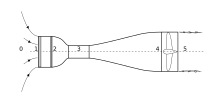
\includegraphics[width=0.90\textwidth]{./fig/wt}
\end{figure}

\sol

\partone
Si studia la galleria a circuito aperto rappresentata in figura utilizzando i bilanci integrali scritti per alcuni volumi di controllo fissi, per ricavare l'andamento della velocità e della pressione all'interno della galleria e infine ricavare la potenza dei motori, necessaria per garantire le condizioni di progetto nella sezione di prova. Si ipotizza un funzionamento stazionario, si trascurano gli effetti viscosi nel volume e sulle pareti della galleria e le forze di volume. In particolare, grazie alle ipotesi fatte, si possono semplificare il bilancio di massa,
\begin{equation}
\begin{aligned}
 & \dfrac{d}{dt} \int_V \rho = - \oint_{S} \rho \bm{u} \cdot \bm{\hat{n}} 
 \hspace{1.0cm} \rightarrow \hspace{1.0cm} \oint_{S} \rho \bm{u} \cdot \bm{\hat{n}} = 0 \ ,
\end{aligned}
\end{equation}
e il bilancio dell'energia cinetica,
\begin{equation}
\begin{aligned}
 \dfrac{d}{dt} \int_V \rho \dfrac{|\bm{u}|^2}{2} & = - \oint_{S} \rho \dfrac{|\bm{u}|^2}{2} \bm{u} \cdot \bm{\hat{n}} + \oint_S \bm{t_n} \cdot \bm{u} - \int_V \bm{\nabla} \bm{u} : \mathbb{T} + \int_V \rho \bm{g} \\
                                                 & = - \oint_{S} \rho \dfrac{|\bm{u}|^2}{2} \bm{u} \cdot \bm{\hat{n}} + \oint_S \bm{t_n} \cdot \bm{u} + 
 \underbrace{\int_V  p \, \bm{\nabla} \cdot \bm{u}}_{=0 \text{, se} \bm{\nabla} \cdot \bm{u} = 0}
 - \underbrace{ \int_V 2 \mu \mathbb{D} : \mathbb{D}}_{=0 \text{, se} \mu = 0} + \int_V \rho \bm{g} \\
 \hspace{1.0cm} \rightarrow \hspace{1.0cm}  &
 - \oint_{S} \rho \dfrac{|\bm{u}|^2}{2} \bm{u} \cdot \bm{\hat{n}} + \oint_S \bm{t_n} \cdot \bm{u} = 0 \ . 
\end{aligned}
\end{equation}

\parttwo
Viene svolta la prima parte dell'esercizio, trascurando le perdite di pressione che avvengono tra la sezione 1 e la sezione 2, a causa della presenza dei nidi d'ape e delle reti.
\newline \noindent
Si scrive il bilancio di massa per un volume di fluido che ha come superficie di contorno la superficie $S_0$, la superficie laterale del tubo di flusso e una superficie $S_i$ all'interno della galleria. Assumendo grandezze uniformi sulla sezione, si può scrivere
\begin{equation}
 \rho A_0 U_0 = \rho A_i U_i \ ,
\end{equation}
cioè che il flusso di massa $\dot{m}$ che attraversa le sezioni della galleria è costante. Se sono note le condizioni di progetto in camera di prova, da esser si può calcolare il flusso di massa,
\begin{equation}
 \dot{m} = \rho A_3 U_3 = \rho A_{test} V_{test} = \dots \ .
\end{equation}
Poiché la velocità all'infinito è nulla, $U_0 \rightarrow 0$, l'area della sezione all'infinito a monte deve tendere all'infinito $A_0 \rightarrow \infty$.
\newline \noindent
Si scrive poi il bilancio di energia cinetica per un volume di controllo che ha come contorno la superficie $S_0$ all'infinito a monte, dove viene aspirata l'aria in uno stato di quiete, la superficie laterale del tubo di flusso, la superficie interna della galleria e la sezione $S_4$ alla fine del divergente, poco prima dell'imbocco dei ventilatori. Poiché non ci sono organi meccanici in movimento, il termine $\oint_S \bm{t_n} \cdot \bm{u}$ è nullo, e assumendo grandezze fisiche costanti sulle sezioni si può scrivere,
\begin{equation}
 \rho A_0 U_0 \left( \dfrac{U_0^2}{2} + \dfrac{P_0}{\rho} \right) =
 \rho A_4 U_4 \left( \dfrac{U_4^2}{2} + \dfrac{P_4}{\rho} \right) \ .
\end{equation}
Poiché il flusso di massa che attraversa le sezioni considerate è costante, il bilancio di energia cinetica si riduce a un'espressione che ricorda quella del teorema di Bernoulli, così come viene enunciato alle scuole superiori,
\begin{equation}
 P_0 + \dfrac{1}{2} \rho \, U_0^2  = P_4 + \dfrac{1}{2} \rho \, U_4^2
 \qquad \rightarrow \qquad B_4 = B_0 = P_{atm} \ ,
\end{equation}
avendo introdotto la definizione del ``binomio di Bernoulli'', $B_i = P_i + \rho U_i^2 / 2$.
\newline \noindent
Si scrive poi il bilancio di energia cinetica per il volume fluido $V(t)$ che contiene il ventilatore, delimintato dalle superifci $S_4$, $S_5$ e la superficie interna della galleria e dalla superficie (mobile!) del ventilatore. Il bilancio diventa
\begin{equation}
\int_{S_4} \rho \dfrac{|\bm{u}|^2}{2} \bm{u} \cdot \bm{\hat{n}} - \bm{t_n} \cdot \bm{u} + 
\int_{S_5} \rho \dfrac{|\bm{u}|^2}{2} \bm{u} \cdot \bm{\hat{n}} - \bm{t_n} \cdot \bm{u} = \int_{S_{fan}} \bm{t_n} \cdot \bm{u} \ ,
\end{equation}
essendo il termine a destra dell'uguale la potenza delle forze essercitata dal ventilatore sul fluido, contraria a quella esercitata dal fluido sul ventilatore, ma uguale a quella che deve fornire il motore elettrico per poter garantire la rotazione del ventialore stesso. Se si trascurano gli sforzi viscosi sulle superfici $S_4$ ed $S_5$, $\bm{t_n} = \bm{s_n} - P \bm{\hat{n}}$, e se si esplicita la potenza che deve essere fornita dai motori, il bilancio diventa,
\begin{equation}
 W_{mot} = 
\int_{S_4} \left( \rho \dfrac{|\bm{u}|^2}{2} + P \right) \left( \bm{u} \cdot \bm{\hat{n}} \right)  + 
\int_{S_5} \left( \rho \dfrac{|\bm{u}|^2}{2} + P \right) \left( \bm{u} \cdot \bm{\hat{n}} \right) \ , 
\end{equation}
e facendo l'ipotesi di grandezze fisiche costanti sulle sezioni,
\begin{equation}
 W_{mot} = \rho A_5 U_5 \left( \dfrac{U_5^2}{2} + \dfrac{P_5}{\rho} \right) 
         - \rho A_4 U_4 \left( \dfrac{U_4^2}{2} + \dfrac{P_4}{\rho} \right)
         = \dot{m} \left( B_5 - B_4 \right) \ . 
\end{equation}
Ricordando che il ``binomio di Bernoulli'' nelle sezioni 1:4 è uguale al ``binomio di Bernoulli'' nella sezione $S_0$, e quindi uguale alla pressione ambiente $P_{atm}$, nell'ipotesi che la pressione nella sezione $S_5$ sia uguale alla pressione atmosferica $P_{atm}$ all'esterno del tubo di flusso, la potenza del motore diventa,
\begin{equation}
 W_{mot} = \dot{m} \dfrac{U_5^2}{2} \ ,
\end{equation}
e, riferendosi alle grandezze fisiche in camera di prova, può essere scritta come
\begin{equation}
\begin{aligned}
 & W_{mot} = \dot{m} \left( \dfrac{A_{test}}{A_{fan}} \right)^2 \dfrac{V_{test}^2}{2} \\
 & \hspace{3.0cm} \rightarrow \qquad 
 W_{mot} = \dfrac{1}{2} \rho A_{test} \left( \dfrac{A_{test}}{A_{fan}} \right)^2 V_{test}^3 = \dots kW \ .
\end{aligned}
\end{equation}
La formula della potenza dei motori necessaria al funzionamento della galleria mette in evidenza la dipendenza dal cubo della velocità di prova e dal quadrato del rapporto tra l'area della sezione di prova e l'area della sezione all'imbocco delle ventole. Questo ultimo termine dovrebbe chiarire uno degli obiettivi del divergente della galleria: rallentare la corrente dopo la sezione di prova, per poter ridurre la potenza dei motori da installare per garantire il funzionamento dell'impianto.
%
\newline \noindent
\textbf{Osservazione.} Potrebbe suscitare qualche perplessità il fatto che la corrente in uscita dall'impianto con velocità $U_5 \simeq V_{fan}$ abbia una pressione uguale alla pressione ambiente, $P_{atm}$, come il fluido in quiete all'esterno del tubo di flusso. {\color{red} Provando ad applicare il teorema di Bernoulli} tra un punto sulla sezione del tubo di flusso $S_5$ e un punto all'esterno del tubo di flusso,
{\color{red}
\begin{equation}
 P_5 + \dfrac{1}{2}\rho V_{fan}^2 = P_5^{out}
 \quad \rightarrow \quad 
 P_{atm} + \dfrac{1}{2}\rho V_{fan}^2 = P_{atm} \ ,
\end{equation}
}
si giungerebbe alla conclusione che {\color{red} $V_{fan} = 0$}. L'errore risiede nell'applicazione del teorema di Bernoulli nella formula vista alla scuola superiore (o in altri corsi universitari), nonostante alcune ipotesi (che verranno presentate nel prosieguo del corso) non siano rispettate. In particolare, per collegare un punto sulla sezione $S_5$ e un punto all'esterno del tubo di flusso viene attraversato uno strato di mescolamento tra la corrente in moto che esce dalla galleria e il fluido in quiete all'esterno: la presenza di questo strato di mescolamento, nel quale la corrente non è irrotazionale $\bm{\omega} \neq 0$, fa cadere le ipotesi del teorema di Bernoulli e lo rende quindi inapplicabile. Tutte {\color{red}le parti evidenziate in rosso devono quindi essere considerate errate}.


% ciclo Otto e potenza di un motore alternativo
\newpage
\noindent
\begin{tabular}{cc}
\begin{minipage}{0.95\textwidth}
\begin{exerciseS}[Motore alternativo]
Il funzionamento di un motore alternativo a benzina (a quattro tempi) può essere rappresentato in prima approssimazione con un ciclo termodinamico Otto ideale, rappresentato da una compressione adiabatica, una fase veloce di combustione a volume costante (nel punto morto superiore del moto del pistone, PMS) e un'espansione adiabatica. Le fasi di aspirazione e scarico dei gas combusti sono anch'essi ideali. L'aspirazione avviene a pressione costante durante il movimento del pistone dal PMS al punto morto inferiore (PMI). La fase di scarico avviene in due fasi: durante la prima fase la pressione diminuisce molto velocemente (approssimata da una trasformazione a volume costante) a causa dell'apertura della valvola di scarico quando il pistone si trova al PMI; durante la seconda fase i gas combusti sono spinti fuori dalla camera di combustione dal movimento ascendente del pistone che si riporta al PMS, per l'inizio del ciclo termodinamico successivo. Del motore sono noti:
\begin{itemize}
 \item il rapporto di compressione, definito come il rapporto tra il volume massimo (pistone al PMI) e minimo (pistone al PMS) della camera di combustione, $r = V_1 / V_2 = 10$;
 \item la cilindrata, definita come la corsa del pistone per l'area della sezione del cilindro, e uguale alla differenza $C = N (V_2 - V_1) = 1000 \ cc$, essendo $N$ il numero di cilindri del motore;
 \item le condizioni termodinamiche dell'aria all'aspirazione $P_0 = 85570 \, Pa$, $T_0 = 25°C$;
 \item il rapporto in massa tra benzina e aria, $f = m_f / m_a = 0.06$;
 \item il potere calorifico della benzina usata $\Delta h = 43 \, MJ$;
 \item la pressione nel basamento del motore, $p_{b} = 150000 \, Pa$ uniforme e costante.
Si calcoli la potenza media erogata dal motore a un regime di rotazione di $\Omega = 3000 RPM$, assumendo un rendimento meccanico $\eta = 0.8$.
Si rappresenti l'aria come un gas bi-atomico perfetto ($\gamma = c_P/ c_v = 1.4$) con costante dei gas $R = 287 J / (kg \, K)$, e si trascuri l'effetto del carburante sul valore dei calori specifici e sulla massa presente all'interno della camera di combustione. Si trascurino inoltre gli scambi di calore per conduzione con l'esterno del cilindro durante la compressione e l'espansione (trasformazioni adiabatiche). Si trascurino i termini cinetici nell'energia totale in camera di combustione, facendo coincidere l'energia totale con l'energia interna $e^t = e = c_v T$, e si assuma che le variabili termodinamiche siano uniformi (costanti in spazio, non in tempo) in camera di combustione.
\end{itemize}
\end{exerciseS}
\end{minipage}
\end{tabular}
\begin{figure}[h]
 \centering
 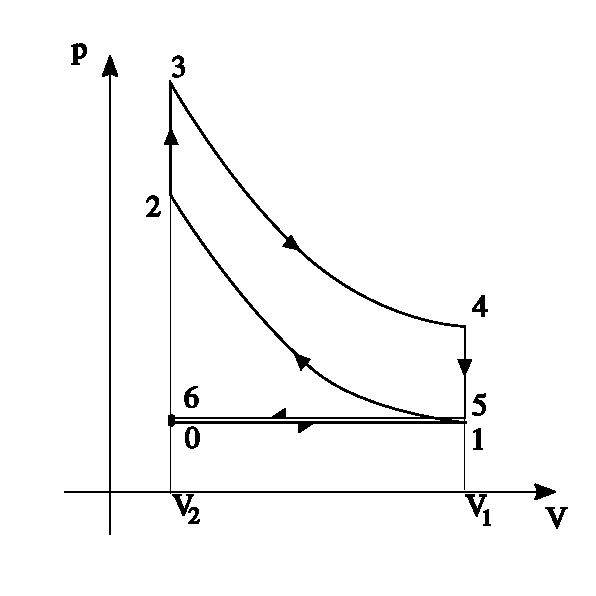
\includegraphics[width=0.45\textwidth]{./fig/otto_cycle}
\end{figure}

% todo: figure with the cut-out of the cylinder, thermodynamic cycle

%
\sol

% Concetti
\partone
Ogni fase del ciclo termodinamico viene analizzata con i bilanci integrali, per il volume corrispondente alla camera di combustione di un cilindro. Questo volume è un sistema aperto durante la fase di aspirazione e scarico (scambia massa con l'esterno), mentre è un sistema chiuso durante la compressione, la combustione e l'espansione (valvole chiuse, nessuno scambio di massa con l'esterno). Si calcola il lavoro svolto dal sistema durante un ciclo e si divide per il periodo per ricavare la potenza media. 

% Svolgimento
\parttwo
Conoscendo il numero dei cilindri $N=3$, il rapporto di compressione $r$ e la cilindrata $C$ è possibile ricavare il valore del volume massimo $V_1$ e minimo $V_2$ della camera di combustione.
\begin{equation}
\begin{cases}
 N( V_2 - V_1 ) = C \\
 V_1 / V_2 = r
\end{cases} \qquad \rightarrow \qquad
\begin{cases}
 V_1 = \dfrac{r}{r-1} \dfrac{C}{N} \\ \\ 
 V_2 = \dfrac{1}{r-1} \dfrac{C}{N}
\end{cases} 
\end{equation}
Si analizzano ora le fasi del ciclo termodinamico, fornendo una breve descrizione e ponendo attenzione allo scambio di massa (sistema chiuso/aperto), lavoro e calore con l'esterno.
\begin{itemize}
\item \textbf{Aspirazione}, $0 \rightarrow 1$: la prima fase del ciclo Otto è l'aspirazione. Durante la fase di aspirazione (ideale), la valvola di aspirazione è aperta e il sistema scambia massa con l'esterno: il pistone si sposta dal PMS al PMI e la camera di combustione si riempie d'aria a pressione e temperatura costante,
\begin{equation}
 p_1 = p_0 \qquad , \qquad
 T_1 = T_0 \qquad , \qquad
 \rho_1 = \rho_0 = \dfrac{p_0}{R T_0} =
\end{equation}
La massa contenuta nella camera di combustione alla chiusura della valvola, in coincidenza del PMI, è
\begin{equation}
 m = \rho_1 V_1 = \dots \ .
\end{equation}
Durante la fase di aspirazione, il pistone deve vincere la sovrapressione del basamento (di solito la pressione nel basamento è superiore a quella aspirata in camera di combustione). Dal PMS al PMI un pistone assorbe parte della potenza fornita dagli altri pistoni. Il lavoro che assorbe è $L_{01} = -(p_b-p_0) \, c$ (negativo poichè assorbito), essendo $c$ la corsa del pistone e la differenza di pressione costante durante l'aspirazione. Questo lavoro assorbito durante l'aspirazione sarà uguale e contrario a quello fornito durante lo scarico ideale dei gas,  che avviene alla stessa differenza di pressione con un moto opposto.
\item \textbf{Compressione}, $1 \rightarrow 2$: la seconda fase del ciclo termodinamico è la compressione del fluido che avviene a causa del movimento verso l'alto del pistone. Il sistema è chiuso: le valvole sono chiuse e si ipotizza che non ci sia trafilamento (\textit{blow-by}) tra il pistone e la superficie laterale del cilindro. Il bilancio di energia totale per il fluido contenuto all'interno del volume $V(t)$ (variabile nel tempo, a causa del moto del pistone) della camera di combustione,
\begin{equation}
 \dfrac{d}{dt} \displaystyle\int_{V(t)} \rho e^t + \oint_{S(t)} \rho e^t (\bm{u}-\bm{v}) \cdot \bm{\hat{n}}= \int_{V(t)} \bm{f} \cdot \bm{u} + \oint_{S(t)} \bm{t_n} \cdot \bm{u} - \oint_{S(t)} \bm{q} \cdot \bm{\hat{n}} + \int_{V(t)} \rho r \ .
\end{equation}
può essere semplificato, trascurando l'effetto delle forze di volume, $\bm{f} = \bm{0}$, trascurando la trasmissione del calore con l'esterno (trasformazione adiabatica), $\bm{q} \cdot \bm{\hat{n}} = 0$, e non essendoci sorgenti di calore, $r = 0$. Inoltre non c'è flusso di massa attraverso il contorno $S(t)$ del volume, $(\bm{u}-\bm{v}) \cdot \bm{\hat{n}} = 0$, e l'unica superficie in movimento della camera di combustione corrisponde al cielo (la faccia superiore) del pistone, $S_{c}$. Trascurando il contributo cinetico e approssimando l'energia totale $e^t = e + |\bm{u}|^2/2$ con l'energia interna $e$, il bilancio di energia diventa,
\begin{equation}
 \dfrac{d}{dt} \displaystyle\int_{V(t)} \rho e = \int_{S_c(t)} \bm{t_n} \cdot \bm{u} \ ,
\end{equation}
legando la derivata temporale dell'energia del fluido nella camera di combustione alla potenza delle forze esercitate dal pistone sul fluido. La potenza delle forze agenti sul pistone è uguale all'integrale superficiale del prodotto scalare vettore sforzo $\bm{t_{n,s}}$ agente sul solido per la velocità $\bm{v}$ della superficie del solido,
\begin{equation}
\begin{aligned}
 W_{12} = \oint_{S_{s}} \bm{t_{n,s}} \cdot \bm{v}
 & = \int_{S_{s,c}} \bm{t_{n,s}} \cdot \bm{v} + \int_{S_{s,b}} \bm{t_{n,s}} \cdot \bm{v}  + \int_{S_{s,lat}} \bm{t_{n,s}} \cdot \bm{v} = \\
 & = - \int_{S_{c}} \bm{t_{n}} \cdot \bm{u} - \int_{S_{s,b}} p_b\bm{\hat{n}_{s}} \cdot \bm{v} \ ,
\end{aligned}
\end{equation}
avendo suddiviso la superficie del cilindro $S_s$ come l'unione della superficie superiore $S_{s,c}$ (cielo), superficie laterale $S_{s,lat}$ (dal contributo nullo, per simmetria), e superifice inferiore $S_{s,b}$ esposta verso il basamento del motore, sulla quale agisce uno sforzo dovuto alla pressione $p_b$ dell'ambiente all'interno del basamento. \'E stato indicata con $\bm{\hat{n}_s}$ la normale uscente dalla superficie del solido e con $\bm{t_{n,s}}$ il vettore sforzo agente su un punto della superficie del solido, uguale e contrario a quello agente sul fluido $\bm{t_n} = -\bm{t_{n,s}}$ per il principio di azione e reazione. Inoltre, le condizioni al contorno impongono che il fluido e il solido abbiano la stessa velocità $\bm{u} = \bm{v}$ sulle superfici di contatto.
Si può quindi riscrivere il bilancio di energia del fluido in funzione della potenza $W_{12}$ trasmessa al pistone,
\begin{equation}
  \dfrac{d}{dt} \displaystyle\int_{V(t)} \rho e = - W_{12} - p_b S_{c} \ v(t) = - W_{12} - p_b \dfrac{d V}{d t} \ ,
\end{equation}
essendo $v(t)$ la velocità del pistone, per ottenere la potenza trasmessa al pistone dal fluido (sarà una potenza richiesta, $<0$),
\begin{equation}
\begin{aligned}
  W_{12}(t) & = - \dfrac{d}{dt} \displaystyle\int_{V(t)} \rho e - p_b \dfrac{d V}{d t} = \\
  & = - \dfrac{d}{dt} \left( \rho V e \right) - p_b \dfrac{d V}{d t} = \\
  & = - m \dfrac{d e}{d t} - p_b \dfrac{d V}{d t} \ ,
\end{aligned}
\end{equation}
nell'ipotesi di variabili termodinamiche uniformi nel volume, ricordando che la massa contenuta nella camera di combustione $m = \rho V$ rimane costante, essendo un sistema chiuso, se si trascura l'effetto di trafilamento tra le pareti di cilindro e pistone (ridotte al minimo da fasce elastiche e anelli raschiaolio sul pistone e sovra-pressione nel basamento).
\newline \noindent
Integrando in tempo la potenza istantantea $W_{12}(t)$, tra il punto 1 e il punto 2 del ciclo, si ottiene il lavoro di compressione
\begin{equation}
 L_{12} = - m (e_2 - e_1) - p_b ( V_2 - V_1 ) \ .
\end{equation}
Utilizzando la legge di stato dei gas perfetti $p = \rho R T$ e il legame tra le variabili termodinamiche durante una trasformazione adiabatica $p/\rho^\gamma = \text{cost}$, si ottiene
\begin{equation}
 e_2 - e_1 = c_v ( T_2 - T_1 ) = c_v T_1 \left[ \left( \dfrac{\rho_2}{\rho_1} \right)^{\gamma-1} - 1 \right] = c_v T_1 \left( r^{\gamma-1} - 1\right) \ .
\end{equation}

\item \textbf{Combustione}, $2 \rightarrow 3$: la terza fase del ciclo termodinamico è la combustione. Viene iniettato il combustibile all'interno della camera di combustione, innescata dall'accensione di una candela in un motore a benzina classico. Durante l'iniezione del combustibile il sistema è aperto. In prima approssimazione si può trascurare la variazione di massa, $m + m_f = m ( 1 + f ) \simeq m$. In prima approssimazione, si può rappresentare questa fase con una trasformazione isocora (volume costante) associata a un aumento di pressione e temperatura, a causa di una combustione (completa) veloce in corrispondenza del PMS. Il bilancio di energia che descrive questa fase diventa
\begin{equation}
\begin{aligned}
 \dfrac{d}{dt} \displaystyle\int_{V(t)} \rho e & = \int_{V(t)} \rho r \\
 m \dfrac{d e}{d t} & = \dot{m}_f \Delta h \qquad \rightarrow \qquad
 e_3 - e_2 = \dfrac{ m_f }{ m } \Delta h  = f \Delta h \ .
\end{aligned}
\end{equation}
Utilizzando l'espressione dell'energia interna $e = c_v T$,
\begin{equation}
 c_v T_3 = c_v T_2 + f \Delta h \ .
\end{equation}

\item \textbf{Espansione}, $3 \rightarrow 4$: la quarta fase del ciclo è l'espansione. Trascurando gli scambi di calore con l'esterno, la trasformazione è adiabatica. Facendo le stesse ipotesi fatte per la fase di compressione, si ottiene un lavoro di espansione (fornito al pistone, $>0$)
\begin{equation}
 L_{34} = -m (e_4-e_3) - p_b ( V_4 - V_3 ) \ .
\end{equation}
Utilizzando la legge di stato dei gas perfetti $p = \rho R T$ e il legame tra le variabili termodinamiche durante una trasformazione adiabatica $p/\rho^\gamma = \text{cost}$, si ottiene
\begin{equation}
\begin{aligned}
 e_4 - e_3 & = c_v ( T_4 - T_3 ) = \\
  & = c_v T_3 \left[ \left( \dfrac{\rho_4}{\rho_3} \right)^{\gamma-1} - 1 \right] = \\
  & = c_v T_3 \left( r^{-\gamma+1} - 1\right) = \\
  & = c_v T_2 \left( r^{-\gamma+1} - 1\right) +
   f \Delta h \left( r^{-\gamma+1} - 1\right)  = \\ 
  & = c_v T_1 \left( 1 - r^{ \gamma-1}\right) +
   f \Delta h \left( r^{-\gamma+1} - 1\right)  = \ .
\end{aligned}
\end{equation}

\item \textbf{Scarico}, $4 \rightarrow 5, 5 \rightarrow 6$: la fase di scarico (libera) è considerata istantanea e quindi non viene compiuto lavoro da parte del fluido sul sistema meccanico. Durante la fase di scarico forzata, mentre si muove dal PMI al PMS, il pistone compie un lavoro $L_{46} = (p_b - p_0) c$, uguale e contrario a quello compiuto durante la fase di aspirazione se la pressione di aspirazione e di scarico sono uguali ($p_0 = p_1 = p_5$).

\end{itemize} \vspace{0.2cm}
%
\noindent
Il lavoro complessivo fornito dal fluido al sistema meccanico durante un ciclo è quindi uguale a 
\begin{equation}
\begin{aligned}
 L = L_{12} + L_{34} & = \dots = \\
 & = f \, m \, \Delta h \left( 1 - r^{-\gamma+1}\right)  \ .
\end{aligned}
\end{equation}
Il risultato ottenuto può essere facilmente interpretato in termini termodinamici, essendo $Q_{in} = f \, m \, \Delta h$ il calore fornito alla macchina termica e $\eta = 1 - r^{-\gamma+1}$ il rendimento del ciclo Otto espresso in funzione del rapporto di compressione $r$,
\begin{equation}
  L = \eta \, Q_{in} \ .
\end{equation}
Nonostante il risultato ottenuto non sia nuovo, lo svolgimento dovrebbe fornire uno svolgimento più dettagliato che parta dai principi fisici, rappresentati dai bilanci integrali, ed evidenziare il ruolo delle ipotesi fatte per ricavare il risultato, come ad esempio l'assenza di flussi di calore durante la fase di compressione e espansione adiabatica. 
%
\newline \noindent
%
Per ottenere la potenza media fornita dal motore, bisogna moltiplicare il lavoro $L$ fornito da un pistone per il numero $N$ dei cilindri del motore e dividere per il periodo del ciclo $T = \dfrac{2 \pi}{\Omega} \dfrac{n}{2}$, essendo $\Omega$ la velocità di rotazione dell'albero motore ed $n = 4$ il numero dei tempi del motore,
\begin{equation}
 W = \dfrac{N L}{T} = \dfrac{\Omega }{n \pi} \, f \, \Delta h \, \rho_1 N V_1 \, \left( 1 - r^{1-\gamma} \right) \ ,
\end{equation}
e introducendo la definizione di cilindrata,
\begin{equation}
 W = \dfrac{N L}{T} = \dfrac{\Omega }{n \pi} \, f \, \Delta h \, \rho_1 C \dfrac{r}{r-1} \, \left( 1 - r^{1-\gamma} \right) = 43.14 \, kW = 58.6 \, CV \ .
\end{equation}


% ciclo Joule-Brayton: matching compressore-turbina, spinta motore
% a getto, ...
\newpage
\noindent
\begin{tabular}{cc}
\begin{minipage}{0.95\textwidth}
\begin{exerciseS}[Motore a getto]
 Un aereo vola alla velocità $V=250 \, m/s$ alla quota $z=10000 \, m$, dove la pressione e la temperatura atmosferica sono $P_0 = 26500 \, Pa$ e $T_0 = 223.25 \, K$, spinto dal motore a getto rappresentato in figura. Sapendo che:
 \begin{itemize}
  \item $0 \rightarrow 1$: la presa d'aria è progettata per ottenere una compressione adiabatica ideale (isentropica), con $P_1/P_0 = 1.5$;
  \item $1 \rightarrow 2$: il compressore ideale ha una sezione di ingresso $A_1 = \dots$ e produce un rapporto di pressione totale $P_2^t/P_1^t = 40.0$, tramite una trasformazione adiabatica ideale;
  \item $2 \rightarrow 3$: il combustore garantisce una perfetta combustione mantenendo costante la pressione totale al suo interno $P_2^t = P_3^t$; il flusso di calore prodotto dalla combustione è uguale a $\dot{Q}_c = \dot{m}_f \Delta h_c$, dove $\dot{m}_f$ è il flusso di massa di combustibile e $\Delta h_c = 46 \, MJ/kg$ il suo potere calorifico; la temperatura totale all'ingresso della turbina è $T_4^t = 1600 \, K$;
  \item $3 \rightarrow 4$: nella turbina avviene un'espansione adiabatica ideale, in modo tale da garantire la potenza necessaria a mantenere in moto il compressore;
  \item $4 \rightarrow 5$: nell'ugello avviene un'espansione adiabatica ideale, che porta il gas a espandersi fino alla pressione ambiente $P_5 = P_0$.
 \end{itemize}
 Si considerino tutti i componenti meccanici ideali, si trascurino gli effetti viscosi dove possibile e si consideri l'aria e la miscela di gas combusti come un gas biatomico ideale, con costante dei gas $R = 287 \, J/(kg \, K)$ e calori specifici costanti.
 \newline \noindent
Viene chiesto di calcolare:
\begin{itemize}
 \item il rapporto in massa tra flusso di combustibile e flusso di aria, $f = \dot{m}_f / \dot{m}_a$;
 \item la spinta $T$ fornita dal motore.
\end{itemize}
\end{exerciseS}
\end{minipage}
\end{tabular}
\begin{figure}[h!]
 \centering
 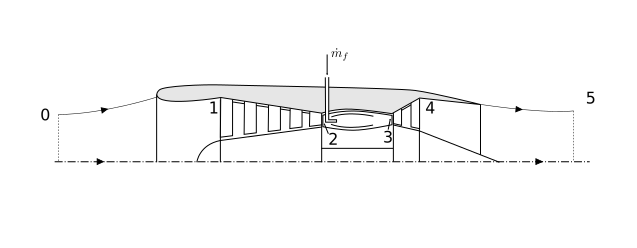
\includegraphics[width=0.95\textwidth]{./fig/jet_engine}
\end{figure}

\sol

\partone
Durante lo svolgimento dell'esercizio vengono utilizzati i bilanci integrali di massa,
\begin{equation}
 \dfrac{d}{dt} \displaystyle\int_{V(t)} \rho + \oint_{S(t)} \rho (\bm{u}-\bm{v}) \cdot \bm{\hat{n}} = 0 \ ,
\end{equation}
quantità di moto,
\begin{equation}
 \dfrac{d}{dt} \displaystyle\int_{V(t)} \rho \bm{u} + \oint_{S(t)} \rho \bm{u} (\bm{u}-\bm{v}) \cdot \bm{\hat{n}}= \int_{V(t)} \bm{f} + \oint_{S(t)} \bm{t_n} \ ,
\end{equation}
ed energia totale,
\begin{equation}
 \dfrac{d}{dt} \displaystyle\int_{V(t)} \rho e^t + \oint_{S(t)} \rho e^t (\bm{u}-\bm{v}) \cdot \bm{\hat{n}}= \int_{V(t)} \bm{f} \cdot \bm{u} + \oint_{S(t)} \bm{t_n} \cdot \bm{u} - \oint_{S(t)} \bm{q} \cdot \bm{\hat{n}} + \int_{V(t)} \rho r \ .
\end{equation}
In particolare, il bilancio di quantità di moto permette di ricavare la formula della spinta del motore in funzione del flusso di quantità di moto attraverso un volume di controllo opportunamente scelto. Il bilancio di energia totale permette di analizzare i singoli componenti del motore. 

\vspace{0.5cm}
\parttwo
Per risolvere il problema, è necessario ricavare la spinta del motore in funzione della portata massica trattata e della differenza di velocità del fluido in ingresso e in uscita dal motore. Successivamente viene analizzato il sistema motore per calcolare la velocità di efflusso dei gas. Si considera il problema stazionario, con forze di volume $\bm{f}$ trascurabili. Si svolge uno studio ``quasi-1D'' considerando variabili uniformi sulle varie sezioni del motore.
%
% \newline \noindent \textbf{Formula della spinta.}
\paragraph{Formula della spinta.}
Nell'ipotesi che la pressione dei gas in uscita dall'ugello sia uguale alla pressione ambiente, il bilancio di quantità di moto del fluido trattato dal motore permette di ottenere la stima della trazione generata dal motore,
\begin{equation}
 T = \dot{m}_5 V_5 - \dot{m}_0 V_0 = \dot{m}_0 ( V_5 - V_0 ) + \dot{m}_f V_5 \ .
\end{equation}
Per ricavare la trazione $T$ è necessario ricavare i valori del flusso di massa d'aria ingerito dal motore, il flusso di combustibile e la velocità di efflusso dei gas combusti, studiando in dettaglio il fluido all'interno del motore
% 
% \newline \noindent \textbf{Analisi del motore.}
\paragraph{Analisi del motore.}
Si studia l'evoluzione della corrente che attraversa il motore.
\begin{itemize}
 \item $0 \rightarrow 1$, presa d'aria: l'aria che approccia l'ingresso del compressore $S_1$ subisce una compressione libera adiabatica ideale. Dato lo stato termodinamico TD(0), con $\rho_0 = P_0/ (R T_0) = 0.414 \, kg/m^3$, e il rapporto di pressione $P_1 / P_0$, è possibile calcolare lo stato termodinamico TD(1):
 \begin{equation}
   P_1 = \left( \dfrac{P_1}{P_0} \right) P_0 = 39750 \, Pa \qquad , \qquad
\rho_1 = \left( \dfrac{P_1}{P_0} \right)^{\frac{1}{\gamma}} \rho_0 = 0.553 \, kg/m^3 \ .
 \end{equation}
Una volta note la pressione e la densità, è possibile calcolare la temperatura e l'entalpia del fluido,
\begin{equation}
 T_1 = \dfrac{P_1}{R T_1} = 250.67 \, K \qquad , \qquad h_1 = c_P T_1 = 2.52 \cdot 10^5 \, J/kg \ .
\end{equation}
Si calcola ora il flusso di massa che entra nel volume,
\begin{equation}
  \dot{m}_0 = \dot{m}_1 \qquad , \qquad \rho_0 V_0 A_0 = \rho_1 V_1 A_1 \ .
\end{equation}
Si calcola il flusso di massa utilizzando la sezione 1. Poiché non ci sono organi meccanici che assorbono o forniscono potenza, non ci sono sorgenti di calore e possono essere trascurati gli effetti viscosi, tra le sezioni 0 e 1 si conserva il flusso di entalpia totale,
\begin{equation}
  \dot{m}_0 h_0^t = \dot{m}_1 h_1^t 
  \quad \rightarrow \quad h_0^t = h_1^t = h_1 + \dfrac{V_1^2}{2} = 2.56 \cdot 10^5 \, J/kg \ .
\end{equation}
\begin{equation}
\begin{aligned}
 \rightarrow \qquad V_1 & = \sqrt{2(h_0^t - h_1)} = 86.09 \, m/s \\
 \dot{m}_1 & = \rho_1 A_1 V_1 = 47.57 \, kg/s \\
\end{aligned}
\end{equation}
 \item $1 \rightarrow 2$, compressore: lo stato termodinamico totale in uscita del compressore è legato allo stato totale in ingresso da una trasformazione isentropica,
 \begin{equation}
   P_2^t = \left( \dfrac{P_2^t}{P_1^t} \right) P_1^t = 1.67 \cdot 10^6 \, Pa \qquad , \qquad
   T_2^t = \left( \dfrac{P_2^t}{P_1^t} \right)^{\frac{\gamma-1}{\gamma}} T_1^t = 729.76 \, K \ .
 \end{equation}
% Una volta note la pressione e la densità, è possibile calcolare la temperatura e l'entalpia del fluido,
% \begin{equation}
%  T_1 = \dfrac{P_1}{R T_1} = \dots \qquad , \qquad h_1 = c_P T_1 = \dots \ .
% \end{equation}
 Trascurando gli effetti viscosi sulla superficie di ingresso e di uscita del compressore, in assenza di scambi di calore, la potenza fornita dal compressore al fluido vale
\begin{equation}
 W_{12} = \dot{m}_1 ( h_2^t - h_1^t ) = 22.72 \, MW \ .
\end{equation}
 \item $2 \rightarrow 3$, combustore: la temperatura totale $T_3^t = \dots$ in ingresso alla turbina è un dato del problema determinato dai limiti tecnologici legati alla realizzazione delle palette del rotore della turbina e al fenomeno di creeping. Nel combustore non ci sono organi meccanici in movimento che forniscano o assorbano potenza dal fluido. Si trascurano gli effetti viscosi e le forze di volume. Se si ipotizza la combustione completa del comustibile iniettato come origine del calore generato e si trascura il flusso di entalpia totale attraverso l'iniettore, il bilancio di energia totale in regime stazionario diventa
\begin{equation}
  \dot{m}_3 h_3^t - \dot{m}_2 h_2^t - \underbrace{\dot{m}_f h_f^t}_{\approx 0} = \dot{Q}_c = \dot{m}_f \Delta h_c
 \ .
\end{equation}
Poiché il flusso di massa dei gas combusti uscenti dal combustore $\dot{m}_3$ è uguale alla somma del flusso d'aria $\dot{m}_2$ e il flusso di combustibile $\dot{m}_f$ entranti,
\begin{equation}
  \dot{m}_3 = \dot{m}_2 + \dot{m}_f \ ,
\end{equation}
il rapporto tra il flusso di massa del combustibile e dell'aria diventa,
\begin{equation}
 f := \dfrac{\dot{m}_f}{\dot{m}_2}
    = \dfrac{h_3^t - h_2^t}{\Delta h_c - h_3^t}
    = \dfrac{T_3^t - T_2^t}{\Delta h_c / c_P - T_3^t} = 0.0197  \ .
\end{equation}
Se si ipotizza che la pressione totale rimanga costante all'interno del combustore, lo stato termodinamico totale in uscita dal combustore è determinato dal valore della pressione e della temperatura totale, $P_3^t$ e $T_3^t$,
\begin{equation}
 \rho_3^t = \dfrac{P_3^t}{R T_3^t} = 3.64 \, kg/m^3 \qquad , \qquad h_3^t = c_P T_3^T = 1.61 \cdot 10^6 \, J/kg \ .
\end{equation}
 \item $3 \rightarrow 4$, turbina: la turbina deve generare la potenza $W_{34}$ necessaria a muovere il compressore,
\begin{equation}
  W_{12} + W_{34} = 0 \ .
\end{equation}
 Se si trascurano gli effetti viscosi e si ipotizza un processo adiabatico, la potenza della turbina è uguale alla differenza del flusso di entalpia totale tra l'uscita e l'ingresso della turbina,
\begin{equation}
 W_{34} = \dot{m}_3 ( h_4^t - h_3^t ) \ .
\end{equation}
L'entalpia totale all'uscita della turbina vale
\begin{equation}
  h_4^t = h_3^t - \dfrac{1}{1+f} ( h_2^t - h_1^t ) = 1.13 \cdot 10^6 \, J/kg 
\qquad \rightarrow \qquad T_4^t = 1124.6 \, K \ .
\end{equation}
La trasformazione isentropica lega lo stato termodinamico totale TD(3) in ingresso alla turbina allo stato termodinamico totale TD(4) in uscita,
\begin{equation}
\begin{aligned}
 P_4^t & = \left(\dfrac{T_4^t}{T_3^t} \right)^{\frac{\gamma}{\gamma-1}} P_3^t = 4.87 \cdot 10^5 \, Pa \\
 \rho_4^t & = 1.51 \, kg/m^3 \ .
\end{aligned}
\end{equation}
 \item $4 \rightarrow 5$, ugello: se si considera un'espansione libera nell'ugello ideale, trascurando gli effetti viscosi e gli scambi di calore, il bilancio dell'energia totale in assenza di organi meccanici che generino o assorbano potenza dal fluido equivale alla conservazione del flusso dell'entropia totale,
\begin{equation}
 \dot{m}_4 h_4^t = \dot{m}_5 h_5^t \qquad \rightarrow \qquad h_4^t = h_5 + \dfrac{V_5^2}{2} 
 \qquad \rightarrow \qquad V_5 = \sqrt{2(h_4^t - h_5)} \\
\end{equation}
Se l'ugello non è bloccato la pressione dei gas in uscita è uguale alla pressione atmosferica, $P_5 = P_0$.
La trasformazione isentropica tra 4 e 5, permette di ricavare lo stato termodinamico TD(5),
\begin{equation}
\begin{aligned}
  \rho_5 & = \left( \dfrac{P_5}{P_4^t} \right)^{\frac{1}{\gamma}} \rho_4^t = 0.189 \, kg/m^3 \\
     T_5 & = 489.5 \, K \qquad \rightarrow \qquad h_5 = 4.92 \cdot 10^5 \, J/kg .
\end{aligned}
\end{equation}
La velocità di efflusso dei gas combusti vale quindi
\begin{equation}
 V_5 = \sqrt{2(h_4^t - h_5)} = 1129.6 \, m/s .
\end{equation}
\end{itemize}
%
La spinta fornita dal motore in questa condizione di volo vale
\begin{equation}
 T = \dot{m}_5 V_5 - \dot{m}_0 V_0 = 42.90 \, kN \ .
\end{equation}















